\documentclass[12pt,twocolumn]{article}

% Page dimensions
\setlength{\hoffset}{-0.4in}
\setlength{\voffset}{-0.5in}
%\setlength{\headsep}{-0.2in}
\setlength{\oddsidemargin}{0in}
\setlength{\textwidth}{7.4in}
\setlength{\textheight}{8.5in}
\setlength{\columnsep}{0.3in}

% Packages
\usepackage{fancyhdr}
\usepackage{abstract}
\usepackage{amsmath,amssymb} 
\usepackage{subcaption} 
\usepackage[usenames,dvipsnames]{color}
\usepackage{placeins}
\usepackage{hyperref}
\usepackage{sectsty}
\usepackage{enumitem}
\usepackage{todonotes}
\usepackage{lastpage}

\hypersetup{
	colorlinks=false,
	pdfborder={0 0 0},
}

%\usepackage[inline]{showlabels}
%\showlabels[\color{blue}]{cite}
%\showlabels[\color{blue}]{ref}

%% ============================================================

% Macros
%\newcommand{\CHRONO}{{\sffamily{{Chrono}}}}
%\newcommand{\ChronoFEA}{{\sffamily{Chrono}}::FEA}
%\newcommand{\ChronoVehicle}{{\sffamily{Chrono}}::Vehicle}
%\newcommand{\ChronoFSI}{{\sffamily{Chrono}}::FSI}
%\newcommand{\ChronoGranular}{{\sffamily{Chrono}}::Granular}
%\newcommand{\ChronoParallel}{{\sffamily{Chrono}}::Parallel}
%\newcommand{\ChronoDistributed}{{\sffamily{Chrono}}::Distributed}
%\newcommand{\ChronoOpenGL}{{\sffamily{Chrono}}::OpenGL}

\newcommand{\chrono}{Chrono}
\newcommand{\chronomod}[1]{\chrono{}::#1}
\newcommand{\synchrono}{Syn\chrono{}}
\newcommand{\gymchrono}{Gym\chrono{}}
\newcommand{\pychrono}{Py\chrono{}}

\newcommand{\gps}{\textsc{gps}}
\newcommand{\imu}{\textsc{imu}}
\newcommand{\mpi}{\textsc{mpi}}
\newcommand{\lidar}{lidar}
\newcommand{\cpu}{\textsc{cpu}}
\newcommand{\dsrc}{\textsc{dsrc}}
\newcommand{\gpu}{\textsc{gpu}}
\newcommand{\ros}{\textsc{ros}}
\newcommand{\tcp}{\textsc{tcp}}
\newcommand{\fea}{\textsc{fea}}
\newcommand{\api}{\textsc{api}}
\newcommand{\scm}{\textsc{scm}}
\newcommand{\optix}{OptiX}

%% ============================================================

% Styles

\definecolor{my-gray}{gray}{0.4}

% First page header
\fancypagestyle{firststyle} {
	\lhead{}
	\rhead{
	\footnotesize
	\textbf{2020 NDIA GROUND VEHICLE SYSTEMS ENGINEERING AND TECHNOLOGY SYMPOSIUM}\\
	\textbf{\sc Autonomy, Artificial Intelligence \& Robotics (AAIR) Technical Session}\\
	\textbf{\sc August 11-13, 2020 -- Novi, Michigan}	
	}
	\chead{}
	%
	\lfoot{}
	\cfoot{}
	\cfoot{\footnotesize DISTRIBUTION STATEMENT A. Approved for public release; distribution unlimited. OPSEC\#864}
	\rfoot{}
}

% All other pages (header and footer)
\pagestyle{fancy}
\fancyhf{}
\rhead{
	\color{my-gray}
	\footnotesize Proceedings of the 2020 Ground Vehicle Systems Engineering and Technology Symposium (GVSETS)
	}
\cfoot{
	\color{my-gray}
	\footnotesize
	{\FooterTitle}\\
	Page \thepage~of~\pageref{LastPage}
}

\renewcommand{\headrulewidth}{0pt}

% Font and styles for sections
\allsectionsfont{\fontsize{12}{15}\selectfont}

\renewcommand{\abstractname}{ABSTRACT}
\renewcommand{\refname}{REFERENCES}

%% ============================================================


\newcommand{\todo}[1]{\textcolor{red}{\textbf{#1}}}

% highlighting, coloring, etc.
\newcommand{\highlightThis}[1]{\textcolor{red}{{\bf{{#1}}}}}
\newcommand{\highlight}[1]{\textcolor{red}{#1}}
\newcommand{\textcolorRED}[1]{{\textcolor{red}{#1}}}
\newcommand{\textcolorBLACK}[1]{{\textcolor{black}{#1}}}


\newcommand{\softpackage}[1]{{\sffamily{#1}}}
\newcommand{\CHRONO}{{\softpackage{{Chrono}}}}

\newcommand{\sbelNewSolution}[1]{\medskip\noindent{\textit{#1}}}

\newcommand{\gonogo}{{\normalfont\textsc{go/no-go}}\xspace}
\newcommand{\go}{{\normalfont\textsc{go}}\xspace}
\newcommand{\nogo}{{\normalfont\textsc{no-go}}\xspace}
%\newcommand{\chrono}{{\textsl{Chrono}}\xspace}

\newcommand{\Reg}{\textsuperscript{\tiny\textregistered}}

\newcommand{\papertitle}{Enabling Artificial Intelligence Studies in Off-Road Mobility Through Physics-Based Simulation of Multi-Agent Scenarios}

%% ============================================================

\title{\bf\large \MakeUppercase{\papertitle{}}}

\newcommand{\FooterTitle}{\papertitle{}, Negrut, et al.}

\author{	
	{\bf D. Negrut, R. Serban, A. Elmquist, J. Taves, A. Young}\\
	University of Wisconsin -- Madison\\
	Madison, WI
	\and
	{\bf A. Tasora, S. Benatti}\\
	Dipartimento di Ingegneria ed Architettura \\
	University of Parma, Italy
}

\newcommand{\MyAbstract}{\textit{
\noindent 
We describe a simulation environment that enables the design and testing of control policies for off-road mobility of autonomous agents. The environment is demonstrated in conjunction with the design and assessment of a reinforcement learning policy that uses sensor fusion and inter-agent communication to enable the movement of mixed convoys of conventional and autonomous vehicles. Policies learned on rigid terrain are shown to transfer to hard (silt-like) and soft (snow-like) deformable terrains. The enabling simulation environment, which is Chrono-centric, is used as follows: the training occurs in the GymChrono learning environment using PyChrono, the Python interface to Chrono. The GymChrono-generated policy is subsequently deployed for testing in SynChrono, a scalable, cluster-deployable multi-agent testing infrastructure that uses MPI. The Chrono::Sensor module simulates sensing channels used in the learning and inference processes. The software stack described is open source. Relevant movies: \cite{simsPaperGVSETS2020}.
} 
}




%% ============================================================

\begin{document}
\date{}

% ------------------------------------------

\twocolumn[
\maketitle             % full width title
\thispagestyle{firststyle}
\begin{onecolabstract} % ditto abstract
\MyAbstract
\end{onecolabstract}
\vspace{0.1in}
]

\newpage

%% ============================================================

\section{INTRODUCTION}
\label{s:introduction}
Computer simulation has been extensively used in the design and analysis of various automation aspects tied to on-road mobility, see, for instance \cite{carlaAVsim2017}. A similar statement cannot be made for off-road mobility owing to a smaller market and a set of stiff challenges brought along by the task at hand. However, a predictive simulation platform for off-road mobility analysis of autonomous agents (AAs) is very desirable since it can accelerate the engineering design cycle, reduce costs, perform more thorough testing, and produce more performant and safer designs. Simulation is not a silver bullet as it has its limitations, first of all the issue of simulation-to-reality transfer \cite{sim2realGapEssex1995}, which pertains to the failure of control policies derived in simulation to work well in the real world. Furthermore, models are difficult to set up and calibrate, the validation process can be tedious and time consuming, and open source simulation tools that are both predictive and expeditious are not readily available. This contribution addresses the third point. It describes a simulation environment whose stated purpose is to allow the practitioner to gain insights into the operation of AAs (robots and autonomous wheeled or tracked vehicles) in off-road conditions with an eye towards: improving mechanical designs of AAs; and, producing and testing control policies that govern the operations of the AAs. These are topical goals for the Army, see, for instance, \cite{jayakumarAutonomous2011,jayAbhiMarco2015,jayGorsich2018,jayGVSETS2019}, or, for a historical perspective on early contributions, \cite{frederickTARDECrobotics2014}.

There are several ongoing efforts that seek to address the AA simulation issue. In robotics, Gazebo~\cite{gazebo,koenig2004design} is a widely used 3D multi-robot simulator with dynamics.  It is not a simulation engine per se, but a \textit{platform} that exposes several engines: ODE~\cite{ode2015}, Bullet~\cite{bulletPhysicsEngine2020}, DART~\cite{dart2018}, and Simbody~\cite{sherman2011simbody}. Unlike Gazebo, which is open source, CoppeliaSim (formerly V-REP)~\cite{V-REP2013} is a commercial multi-robot simulation solution that also exposes a set of simulation engines: MuJoCo~\cite{todorovMujoco2012}, Vortex Dynamics~\cite{cmLabs2020}, Bullet, and Newton Dynamics~\cite{newtonDynamics2020}. ROAMS~\cite{abhiROAMS2004} and ANVEL~\cite{ANVEL-website} are two other simulation engines for off-road AAs. The former is used for mission planning by NASA and draws on an in-house dynamics engine~\cite{DARTS}; the latter relies on the ODE simulation engine and has been used in the past for off-road military applications~\cite{ANVELdescription2012} in combination with a sensor simulation package~\cite{VANE-2012}. MAVS is an off-road AA simulation environment that is currently under active development \cite{mavsCarruth2018}. It provides an in-house developed, sophisticated sensor simulation module \cite{goodin2018enabling,goodin2019predicting}, has a ROS bridge, and uses Chrono as its dynamics engine. USARSim is an AA simulation platform, not under active development, that draws on a game engine (Unreal Engine~\cite{unrealEngine}), a choice with pluses (scalability, ability to create complex worlds) and minuses (the simulation engine is designed for plausibility rather than accuracy). For autonomous vehicle (AV) simulation, Carla~\cite{carlaAVsim2017} and AirSim~\cite{shah2018airsim} are two often used open-source simulators, the former for on-road AV driving scenarios simulation, the latter originally designed for drones but now including support for on-road traffic of AVs as well. Carla and AirSim rely on Unreal Engine but several other engines are used for AA simulation, e.g. Unity~\cite{unityGaming} and TORCS~\cite{torcsRacingSimulation2020}. For a survey of other solutions for on-road mobility the reader is referred to~\cite{surveyAVsimulationBerger2019,reviewPerception2019}.

The AA off-road mobility simulation platform discussed here is Chrono-centric~\cite{projectChronoWebSite,chronoOverview2016}. In its purpose, it is similar to the ANVEL-VANE environment as it seeks to simulate robots and wheeled/tracked vehicles operating in off-road conditions. Compared to the ANVEL-VANE solution, the Chrono environment is different in several respects: it is open source and available for unfettered use under a BSD3 license; it uses its own multi-physics engine; it is scalable and deployable on supercomputers, clusters, or multi-core architectures owing to its reliance on the MPI message passing standard for parallel computing~\cite{MPI-Forum-1994}; and is under active development. Chrono is an ecosystem of modules and toolkits. It has support for rigid and flexible body dynamics (Chrono::Engine), fluid-solid interaction (Chrono::FSI), and granular dynamics (Chrono::Parallel and Chrono::Granular) applications. It has Python bindings, support for sensor simulation in Chrono::Sensor, an API for ROS~\cite{ROS-2009} bridging, as well as facilities for: rapid vehicle modeling via parameterized templates~\cite{ChronoVehicle2019}; control policy design with GymChrono; and scalable control policy testing with SynChrono. Chrono relies on GPU computing for fluid-solid interaction and select granular dynamics simulations, multi-core for most of the other modules, and MPI-enabled parallel computing for co-simulation when handling large terramechanics applications or collections of AAs. Real-time simulation is not one of Chrono's priorities. Although for vehicle-on-rigid-terrain simulation it provides faster than real-time performance, there are numerous applications that lead to long run times in Chrono, e.g., deformable terrain mobility, nonlinear flexible body dynamics, fording scenarios, etc. 

This contribution highlights the Chrono components that support the design and testing of control policies through simulation: PyChrono, GymChrono, Chrono::Sensor, and SynChrono. To show these components at work, a Reinforcement Learning (RL) approach is used herein to produce a control policy. There is nothing special about the RL approach; other techniques to design control policies could be used equally well, a point touched upon in more detail in Section \S\ref{sec:ML}. Section \S\ref{sec:simInfrastructure} describes the Chrono infrastructure that facilitates artificial intelligence studies in off-road, multi-agent mobility scenarios. Section \S\ref{sec:demoTechnology} covers simulation experiments that highlight two aspects: the scalability of the SynChrono testing environment, and the process of designing the RL control policy along with an evaluation of the policy's robustness. Concluding remarks and directions of future work round off the contribution. 



\section{DERIVING CONTROL POLICIES THROUGH SIMULATION}
\label{sec:ML}
Derived using an accurate simulation framework, control algorithms have been shown to bridge the sim-to-reality gap successfully~\cite{VISTASimMITRL, VirtualToRealRL}. The use of vehicles with Level 1 and Level 2 autonomy has grown considerably~\cite{J3016_201401, SAEHardwareInTheLoop} and the automotive industry is making major strides in the transition to Levels 3 and 4 autonomy~\cite{WayveRLSimToReal, TeslaSummon}. The use of simulation for on-road AVs is an area of intense research and development as this technology is seen as an important catalyst of the aforementioned transition. One active area of research is focused on sampling-based methods. These approaches generate many candidate trajectories a vehicle can follow, selecting and executing the controls associated with the best candidate~\cite{UrbanAVBezierMPC, RRTRealTime}. Graph search methods are commonly associated with each trajectory. The approach is real-time challenged, since achieving robust results requires a high number of samples to be analyzed~\cite{TrajectoryPlanningMIQP}. Algorithms such as Dijkstra's, A-Star (A*), or the Rapidly-exploring Random Tree-Star (RRT*), sample the state space either deterministically or stochastically~\cite{RRTRealTime}. Depending on the complexity of the traffic scenario, these algorithms can prove computationally costly and provide sub-optimal results.

Model Predictive Control (MPC) is another common AV control approach~\cite{Borrelli2005MPCbasedAT}. Using a dynamic model of a vehicle, the MPC algorithm computes trajectories over the state space and determines an optimal trajectory using gradient-descending optimization techniques~\cite{TrajectoryPlanningMIQP, Liniger2017OptimizationBasedAR}. A limited time horizon is employed to reduce unneeded computation for times too far out into the future. In comparison to sampling algorithms, the MPC approaches show improved performance that is tied to the use of the gradient fields in the optimization problem that comes into play~\cite{Borrelli2005MPCbasedAT}.

The accuracy of the simulation platform plays a critical role both for MPC as well as sampling-based controllers. To adequately validate and subsequently verify a controller such as MPC, the simulation must be of high enough definition to carry over successfully to reality~\cite{AVTestingMethods}. When using the more pedestrian PID controller solutions, for which gains must be carefully selected, an inaccurate simulation platform could yield a poor design that leads to undesired consequences when deployed on a real vehicle.

The design of a robust controller that performs adequately in complex environments using the aforementioned strategies has proven difficult when aiming for a generalized policy~\cite{Kuutti2019ASO}. An emerging approach that has gained momentum in recent years is Machine Learning (ML) based \cite{surveyRLrobotics2013}. ML has shown promise in producing efficient and robust models that generalize well in a variety of situations. The three pillars of ML include supervised learning, unsupervised learning, and reinforcement learning. In the AA problem, deep reinforcement learning (DRL) has been very successful, as it displays the ability to learn and respond in complex scenarios without the need for preprocessed or labeled data~\cite{VirtualToRealRL}.

Since its introduction~\cite{Mnih13}, DRL has proven successful in robotics applications~\cite{Levine2016,inHandManipulation2020}. At its core, DRL is an iterative learning process in which an \emph{agent} interacts with an \emph{environment}; at each iteration the agent collects an \emph{observation} (or \emph{state}), then performs an \emph{action} based on the previous observation and gets a \emph{reward} which is a measure of its performance. The goal of RL is to find a policy that maximizes the sum of the collected reward. 

RL allows for complex control policies viable in unstructured and stochastic environments; it is model-free in that it does not require a model that predicts environment transients; and can learn from scratch. RL's major flaw is its need for a massive amount of training data to infer a robust policy. The role of simulation is to produce this collection of samples. \emph{Policy Gradient Algorithms} are a subset of RL algorithms whose goal is to directly learn an optimal stochastic policy $\pi_\theta(a|s)$, where $s$, $a$, and $\theta$ are the state, action, and a set of learnable parameters, respectively. If $\pi$ is a Neural Network (NN), $\theta$ are the weights and biases of the NN, the state is the NN input, and the action is its output. Proximal Policy Optimization (PPO)~\cite{Schulman2017PPO} is one of the most widely used algorithms for continuous state and action environments and will be the algorithm of choice in this contribution. PPO is a policy gradient algorithm whose goal is to optimize a stochastic policy. It is also an actor-critic method since another NN is trained and used to estimate the Value Function~\cite{SuttonBarto1998RL} employed to estimate the Advantage Function~\cite{Kakade02approximatelyoptimal}. The Advantage Function is used in the objective function to be maximized.

\section{SIMULATION INFRASTRUCTURE}
\label{sec:simInfrastructure}
The purpose of the simulation environment described is twofold. First, it is used to produce the data needed to design a control policy. Second, it is used for testing purposes. To this end, it exposes the control policy produced in a model-based or model-free approach to a battery of tests to gauge its correctness and robustness. This section outlines the components of this Chrono-centric simulation environment. The emphasis is placed on four components: Chrono::Sensor, PyChrono, GymChrono and SynChrono, that anchor the AA design and testing process and have not been discussed elsewhere in detail. More established Chrono components or functionality will be touched upon in passing; more details are provided in  \cite{chronoOverview2016,ChronoVehicle2019,ChronoSCM2019}.

\paragraph{Chrono.} Under active development for over two decades, Chrono~\cite{chronoOverview2016} is a multi-physics simulation engine distributed as open-source under a permissive BSD license.  Its core module, Chrono::Engine, provides support for rigid multibody dynamics, nonlinear finite element analysis, and frictional contact dynamics. Chrono is modular, with optional modules providing support for additional classes of physics simulation (e.g., fluid-solid interaction or large-scale granular dynamics), for modeling and simulation of specialized mechanical systems (e.g., ground vehicles), for interfaces to external solvers (e.g., sparse direct linear solvers), or for dedicated parallel algorithms targeting different computing architectures (multi-core, distributed, and GPU) for large-scale simulations.

Written almost entirely in C++, Chrono is middleware and therefore supports customized solutions that involve user code and potentially third-party software. The software is portable and can be built on different platforms, under different operating systems, and using various compilers. Chrono is actively developed, has a continuous integration process, an active user forum, and is managed through GitHub~\cite{projectChronoGithub}. It's latest release is 5.0.1, available as of March 2020.  Chrono is used by academic, industrial, and government research and development groups and projects.

\paragraph{Chrono::Vehicle.} Chrono::Vehicle~\cite{ChronoVehicle2019} is a specialized Chrono module that makes available a collection of templates (fully parameterized models) for various topologies of both wheeled and tracked vehicle subsystems. It provides facilities for modeling rigid, deformable, and granular terrain; support for closed-loop and interactive driver models; and run-time and off-line visualization of simulation results. Chrono::Vehicle leverages and works in tandem with other Chrono modules for run-time visualization or finite element, granular dynamics, and parallel computing support.

Chrono::Vehicle provides vehicle \textit{subsystem} templates for tires, suspensions, steering mechanisms, drivelines, sprockets, track shoes, etc.; templates for external systems such as powertrains, drivers, and terrain models; and additional utility classes and functions for vehicle visualization, monitoring, and collection of simulation results.  As a middleware library, Chrono::Vehicle requires the user to provide C++ classes for a concrete instantiation of a particular template.  An optional Chrono library provides complete sets of template instantiations for several concrete ground vehicles, both wheeled and tracked, which can serve as examples for developing more customized vehicle models. An alternative mechanism for defining concrete instantiation of vehicle system and subsystem templates is based on input specification files in the JSON format \cite{json}.  For additional flexibility and to allow integration of third-party software, Chrono::Vehicle is designed to permit either monolithic simulations or co-simulation where the vehicle, powertrain, tires, driver, and terrain/soil interaction can be simulated independently.

\begin{figure}
    \centering
    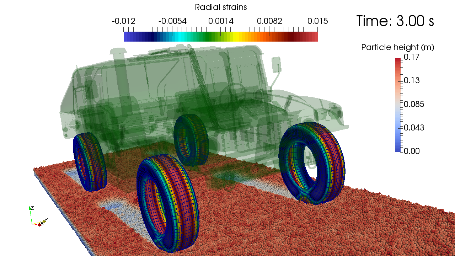
\includegraphics[width=0.8\columnwidth]{Figs/HMMWV-Granular.png}
    \caption{{\small Chrono::Vehicle HMMWV with flexible tires navigating granular terrain demonstrating vehicle dynamics, flexible body dynamics, and parallel computing support in Chrono \cite{antonioVehicleTireGranMatSim2017}.}}   
    \label{fig:hmmwvgranular}
\end{figure}

Chrono::Vehicle provides several classes of terrain and soil models, of different fidelity and computational complexity, ranging from rigid, to semi-empirical Bekker-Wong type models, to complex physics-based models based on either a granular or finite-element based soil representation.  For simple terramechanics simulations, Chrono::Vehicle implements a customized Soil Contact Model (SCM), based on Bekker theory, with extensions to allow non-structured triangular grids, adaptive mesh refinement, and incorporation of bulldozing effects~\cite{ChronoSCM2019}.  Second, Chrono provides an FEA continuum soil model based on multiplicative plasticity theory with Drucker-Prager failure criterion and  specialized brick elements. Finally, leveraging Chrono support for large-scale granular dynamics and for multi-core, GPU, and distributed parallel computing, off-road vehicle simulations can be conducted using fully-resolved, granular dynamics-based complex terramechanics, using a Discrete Element Method approach, see Fig.~\ref{fig:hmmwvgranular} \cite{antonioVehicleTireGranMatSim2017, serbanCosimIJVP2019}.

\paragraph{Chrono::Sensor.} Chrono::Sensor provides sensor simulation support for software-in-the-loop testing. Cameras, lidar, GPS, and IMU sensors can be placed within a Chrono simulation to generate synthetic data based on user-defined sensor parameters and attributes of the virtual world hosting the AA simulation experiment. The goal of the module is to allow realistic data generation based on sensor characteristics such as noise, distortion, and lag. Sensors can be attached to objects within the simulation and configured to match corresponding real sensors. For modeling convenience, sensors can be defined through a JSON file \cite{json}. Additionally, custom sensors and post-processing filtering can be implemented, leveraging the existing render framework or physics interface. 

For interoceptive sensing (GPS and IMU), the module utilizes the internally computed physical quantities from the Chrono system and can augment this ground truth with drift, Gaussian noise, lag, and filtering characteristics from finite collection time. For exteroceptive sensors that provide information about scene characteristics (camera and lidar), Chrono::Sensor leverages hardware accelerated ray tracing through the OptiX library~\cite{optixNVIDIA} and implements physically based rendering techniques. The ray tracing approach allows for the physical reconstruction of the light-based data acquisition process and thus controls the attributes of the synthetically generated sensor data. For camera, lens models and post-processing noise augmentation are supported, with an interface to extend or implement custom models. For lidar, the framework expands on work from~\cite{goodin2018enabling} to provide a beam divergence model that supports multiple modes of lidar return and reduced intensity during partial beam reflectance. The camera and lidar can also be parameterized by update rate, time over which to collect data, and lag. 

Chrono::Sensor is currently in development with planned expansion of sensor support and additional distortion model implementations. All sensors and capabilities are written in C++, but can also be accessed from Python through the PyChrono interface. The entire module can be run headless without the requirement of a render context, allowing for ease of deployment in machine learning applications on remote servers (in the cloud).


\paragraph{PyChrono.} While the main Chrono API is expressed in C++, in recent years a concerted effort was dedicated to providing automatically-generated Python wrappers for much of the Chrono functionality. The purpose was twofold: to provide a lower-entry point to Chrono simulations for users less familiar with C++; and, provide a bridge to various machine learning platforms, e.g. TensorFlow \cite{tensorflow}, PyTorch \cite{paszke2017PyTorch}, Theano \cite{theano2016}, and CAFFE \cite{caffe2014}.  

The Python wrapping relies on using automated technology provided by SWIG \cite{swig2003}, which generates the interface between Python user-code and the underlying Chrono C++ libraries. Presently, a large set of Chrono functionality is exposed to Python users, including the core multibody and FEA module, the interface to CAD systems (like SolidWorks), run-time visualization with Irrlicht, etc. In particular, full support is available for both modeling, simulation, and visualization of wheeled ground vehicles and use of the Chrono::Vehicle existing wheeled vehicle models, as well as using the sensor models provided by Chrono::Sensor. PyChrono for Python 3 can be built from sources on any of the supported platforms (Linux, Windows, MacOS).  Alternatively, pre-built conda PyChrono packages are available on the project's Anaconda page~\cite{pyChronoCondaWebSite} (note that Chrono::Sensor is not available yet via the conda PyChrono packages). 

\paragraph{GymChrono.} GymChrono is an extension of OpenAI Gym~\cite{Brockman16Gym}. It exposes a set of environments providing continuous control tasks for physics and sensor simulation run by the Chrono backend. These environments inherit from OpenAI Gym classes. As such, they can be used out of the box with any algorithm or DRL framework made for gym environments. They can also draw on gym's environment parallelization for learning acceleration.

\paragraph{SynChrono.} SynChrono is a software component that uses Chrono to implement a distributed-memory execution model when simulating scenarios that include multiple AAs. By leveraging the Message Passing Interface (MPI) standard~\cite{mpi-3.0}, SynChrono can manage multiple instances of Chrono running together \textit{one} mobility analysis on a supercomputer, cluster, or multi-core setup thus supporting the scalable and distributed simulation of multiple agents (robots, tracked vehicles, wheeled vehicles, etc.) The paradigm embraced is that of running the dynamics of one AA as one MPI rank, with the ranks/AAs communicating through MPI messages to maintain space and time coherent state for all agents participating in the study. As an example, if there are two agents, SynChrono makes it possible to synchronously run the two agents on two different compute nodes in a supercomputer. By the same token, if there are 50 agents and 50 compute nodes in a cluster, SynChrono provides the infrastructure to keep the 50 agents operating in a coherent (timewise and spacewise) virtual world. Although each agent represents a Chrono simulation, SynChrono makes it possible for ruts generated by agent 27 to be picked up on a camera sensor on agent 31 if the camera points to agent 27. The time coherence aspect prevents some agents from racing into the future while other agents lag behind in the past. The global synchronization mechanism in SynChrono ensures that all 50 agents march forward in simulation time in a coherent fashion so that mutual interaction (a vehicle crossing the ruts of a different one, a vehicle sensing another vehicle, etc.) happens as in real life.

The structure of SynChrono's MPI framework is shown in Fig.~\ref{fig:mpischematic}. SynChrono manages multiple AAs as multiple processes via as many MPI ranks. Each AA runs in its own SynChrono process (an MPI rank) and interfaces with its dedicated control stack for software-in-the-loop control. The control stack is fed synthetic data generated by Chrono::Sensor and acts upon the environment through Chrono::Vehicle control inputs (throttle, steering, braking). The control algorithm for each agent is also configurable and can vary from complex algorithms that fuse sensor feeds/data streams, to controls based on empirical models, and on to pre-recorded driver inputs from a human or human-driven control in scenarios that are simple enough to allow real-time simulation. SynChrono supports human-in-the-loop experiments as well. 

\begin{figure}
	\centering
	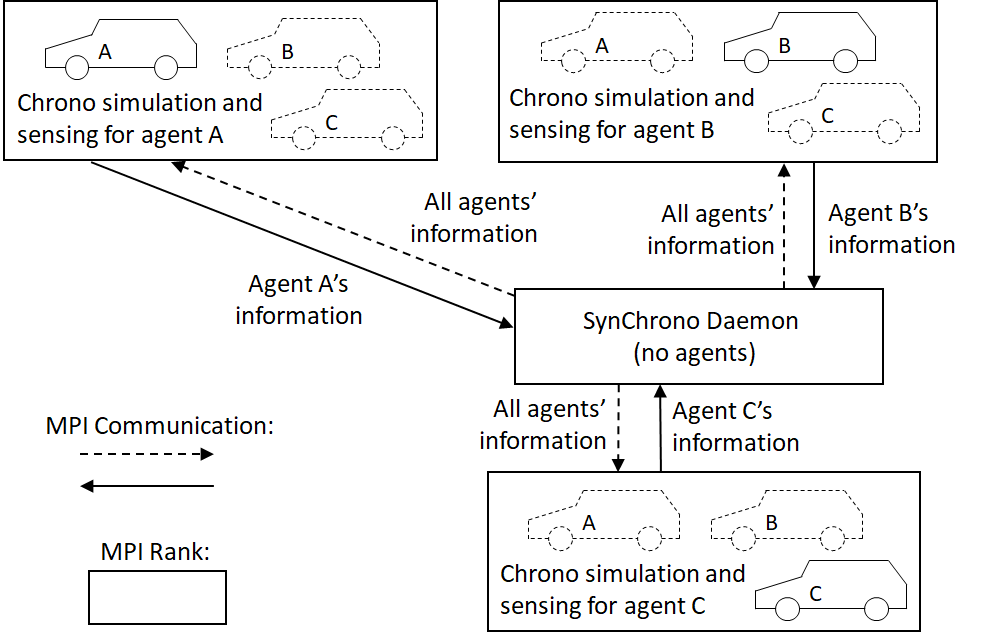
\includegraphics[width=\columnwidth]{Figs/syn_cars_diagram.png}
	\caption{{\small Schematic of the SynChrono framework. Dynamics simulations are done in separate Chrono systems and the outcome of the dynamics simulation is synchronized between ranks using MPI.}}   
	\label{fig:mpischematic}
\end{figure}

Each SynChrono process is responsible for the dynamics of a single agent. At a slow frequency (relative to the simulation time-step), all SynChrono processes communicate via the SynChrono daemon to exchange state information. State information is intended to be brief, sufficient to enable a SynChrono process to reconstruct a ``ghost'' version of outside agents in its own world for visualization and sensing purposes. In an example where each agent is a vehicle, the state information consists of the vehicle location and orientation along with pose information for each wheel. This information is packaged via the FlatBuffers serialization library \cite{flatbuffers}. 

One limitation of the implementation is that currently two agents running as two SynChrono processes cannot crash with each other or participate in an operation that couples their dynamics, e.g. lifting together a heavy object. Such a scenario should be run in Chrono, since the coupling is too tight to be handled by SynChrono. This will make the simulation longer to run since more agents will have to be handled within one Chrono process. However, if the agent coupling happens via sensing or the virtual world, e.g., one agent sensing another one, or one vehicle crossing over and being jolted by the ruts left by a different agent, then SynChrono can be relied on, thus ensuring scalability. The goal of SynChrono is to have virtually constant scaling up to a high threshold where the data passing overhead becomes the simulation bottleneck. 

\paragraph{Interface to an external controller.} For testing of control algorithms that are intended to be easily transferred to real-life vehicles or robots, the simulation platform provides an external control interface that is exposed in SynChrono. An agent in SynChrono can send messages (i.e. sensor data packets) to the external autonomous controls framework which can then send a message back (i.e. control inputs). The control stack is independent of the SynChrono platform (e.g. a bridge has been developed for ROS \cite{ROS-2009}), and can be tested with inputs replicating those from reality, such as sensor and/or V2X communication data.

%% ===========================================================
\section{TECHNOLOGY DEMONSTRATION}
\label{sec:demoTechnology}
All simulation scenarios considered in this section use a Chrono::Vehicle HMMWV model. Chrono::Vehicle was benchmarked as part of the Next Generation-NRMM (NG-NRMM) exercise \cite{NATObenchmark2018}; Chrono::Vehicle-specific benchmark findings are detailed in \cite{TR2017-05NRMM-wheeled,TR2016-08NRMM-tracked}. Note that: the NG-NRMM benchmarking effort involved Chrono::Vehicle but no the particular model used in this study; and, all results reported herein were obtained using a simulation time step of $\Delta t=2 \times 10^{-3}$ seconds, both for rigid and deformable terrain. This time step information is relevant when discussing real-time performance and scalability aspects.

\subsection{SynChrono scaling analysis}\label{sec:syn-scaling-analysis} 
SynChrono uses $N+1$ processes executing on a cluster/supercomputer to simulate the dynamics of $N$ agents handled as $N$ independent Chrono simulations. Each Chrono simulation is a process; the extra process is involved in maintaining the time and space coherence for the virtual world shared by the $N$ AAs. The SynChrono daemon executes as the extra process and it coordinates via MPI the dynamics of the $N$ agents. The numerical experiments described here answer the following questions: ($i$) How does the time to complete a simulation change as $N$ increases? ($ii$) How fast is SynChrono in mobility studies on rigid terrain? ($iii$) How fast is it when an SCM deformable terrain model is considered in the simulation scenario? The Linux cluster used exposed 15 nodes. Thus, one set of experiments was conducted with up to $N=14$ AAs, using rigid, SCM hard (silt-like), and SCM soft (snow-like) terrain, with one agent per compute node. However, the experiment also included scenarios with up to 56 AAs. In this case, four AAs ran on the same compute node. On the upside, this allowed more AAs to participate in the benchmark; on the downside, the simulation times went up since the hardware allocation per AA went down by a factor of four.

The handling of a virtual world that has SCM terrain is challenging since each of the $N$ vehicles changes the terrain at the same time and these changes must be space and time coherent. This is facilitated and managed by the SynChrono daemon. The key component of the SCM terrain is the deformation of each vertex in the underlying SCM mesh. All other terrain properties can be computed based on the height of each vertex alone~\cite{ChronoSCM2019}. At each simulation step, a SynChrono rank that is associated with an agent moving on SCM terrain collects a list of the deformed vertices that the agent produced during the course of that time step. Mesh deformation data may not be sent at every simulation time-step, so this collection of mesh changes is in general persistent across simulation time steps. Once an agent reaches a SynChrono synchronization point, the cumulative mesh deformations produced by one agent are sent via the daemon to every other agent's world. Each agent then applies the deformations to their own copy of the SCM mesh and resets their collection of new mesh deformations. This means that two agents should not come close enough that they deform the same vertices during the same synchronization period, but this is just as restrictive as SynChrono's assumption that any two agents will not interact by crashing. While Chrono's SCM implementation allows for meshes that auto-refine, this is currently not supported in SynChrono due to the significant increase in algorithmic complexity for relatively little gain in performance. The main concern for scalability is message size, since for synchronizing SCM terrain there is about 15 times as much data to send for each agent relative to the rigid terrain case. 

The scenario discussed herein is that of many vehicles crossing perpendicularly on a rectangular patch of SCM terrain, see Fig.~\ref{fig:scalingenv} and online movies \cite{simsPaperGVSETS2020}. In this setup, one can easily scale up the number of vehicles and verify that the SCM terrain deformation is properly synchronized across multiple ranks. The scaling metric used was the Real Time Fraction (RTF), representing the amount of wall-time required to finish a simulation divided by the amount of time simulated. Running in real-time corresponds to a factor of 1, while slower than real-time corresponds to factors larger than one. The tests were run on the Euler computing cluster at the University of Wisconsin-Madison. Each node has an eight core, Broadwell-generation Intel processor; inter-node communication is facilitated via a Gigabit Ethernet interconnect. 

In a first sub-experiment, we assign each SynChrono process (which runs one vehicle) to distinct cluster nodes. The scaling analysis results are presented in Fig.~\ref{fig:scmscaling}. The plot shows on the $y$-axis the $ log_{10} $ of the RTF. Thus, any dot below the horizontal $x$-axis is associated with an experiment that ran faster than real time. Simulations on the rigid terrain ran with an RTF of 0.75 and simulations on either type of SCM terrain (hard or soft) ran with an RTF of approximately 110. The RTF value of 110 is independent of the of SCM soil parameters (i.e. soft vs. hard), but is highly dependent on the processor performance, MPI implementation, compiler, and compilation optimization. These results confirm weak scaling behavior: no significant performance penalty is observed for including additional agents in the simulation when each SynChrono process is assigned to a different compute node. 

\begin{figure}
    \centering
    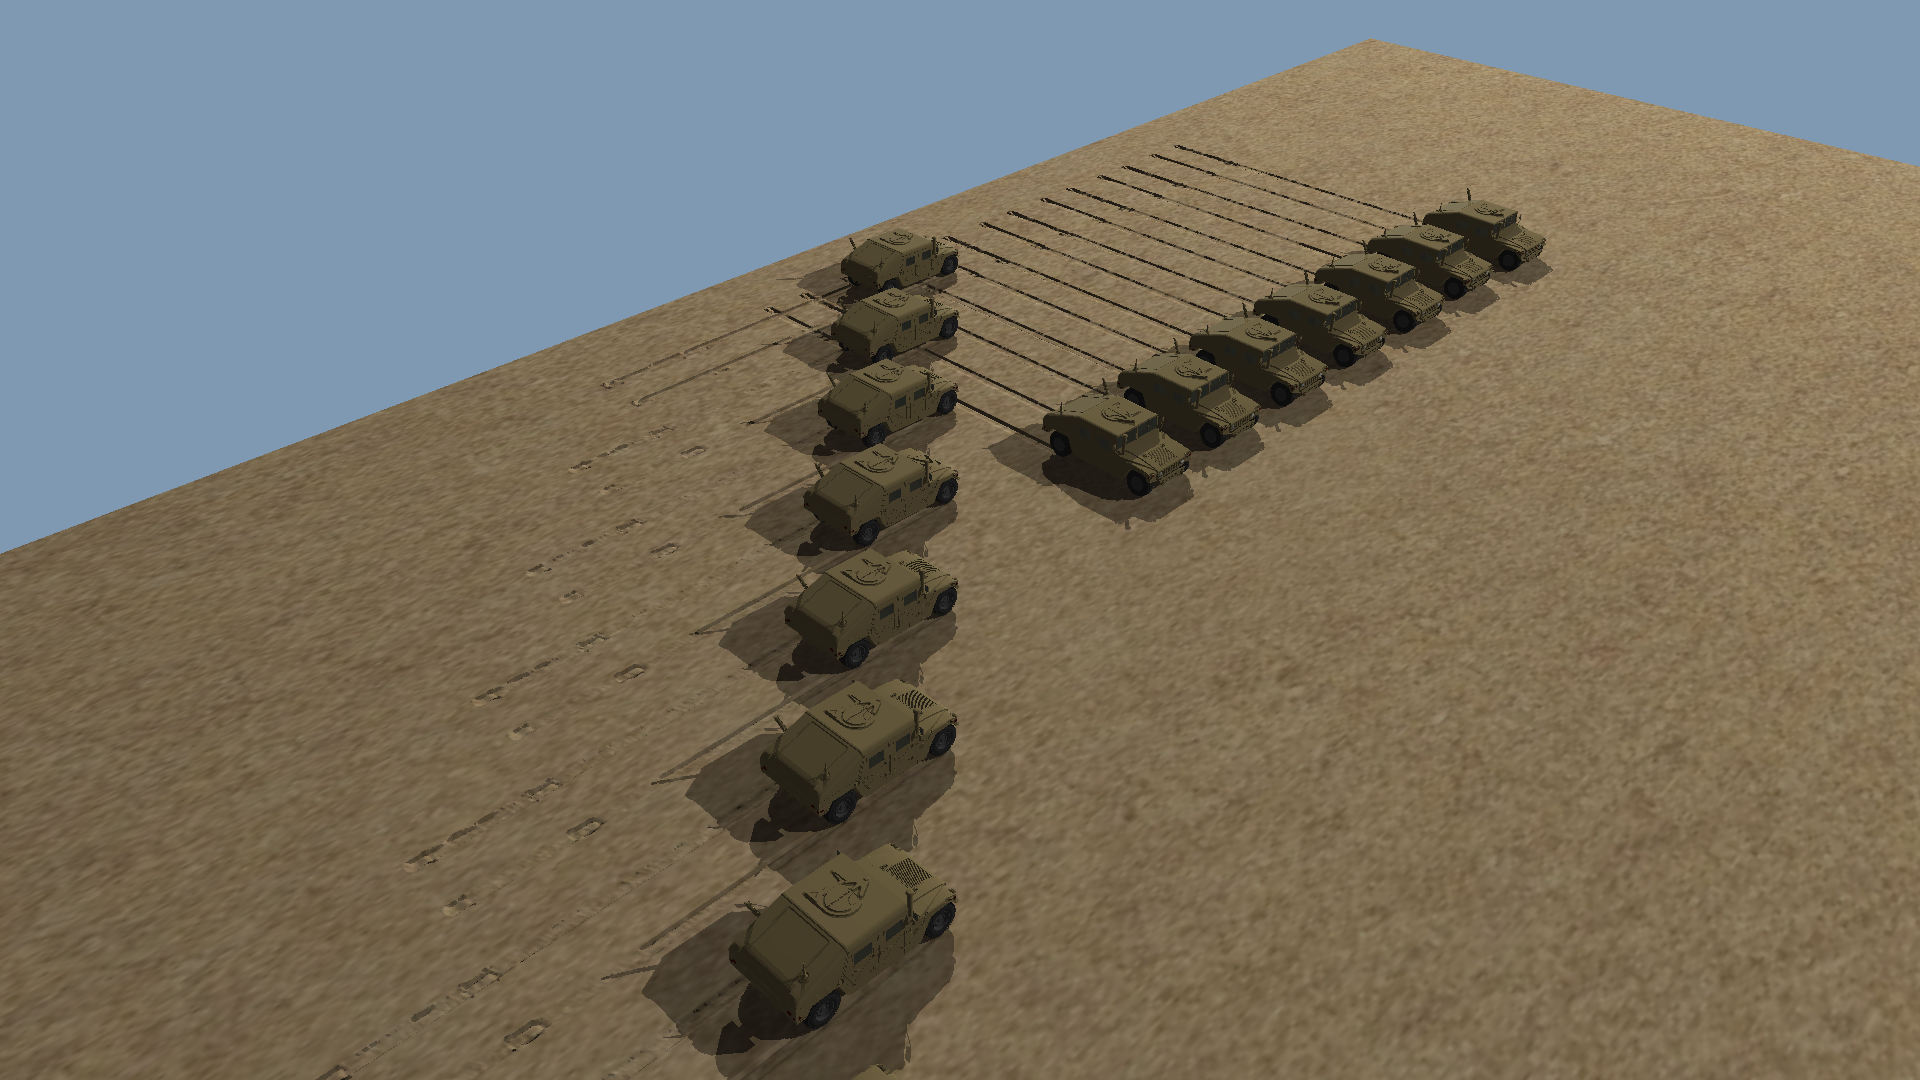
\includegraphics[width=\columnwidth]{Figs/Syn-SCM-setup.png}
    \caption{Environment used for SynChrono scaling analysis for agents operating on SCM terrain. Two lines of vehicles move across a rectangular patch, crossing orthogonally and making ruts in the SCM soil. Simulations were run on both soft and hard SCM terrain, as well as on rigid terrain.}
    \label{fig:scalingenv}
\end{figure}

Using the same scenario as above, scaling analyses were also conducted for a larger number of agents on rigid terrain to ensure that the same weak scaling continued to hold. To this end, two other sub-experiments were conducted: two SynChrono processes were deployed per node; and, four SynChrono processes were deployed per node. Given the number of nodes made available on the cluster (15), for two-per-node, SynChrono handled 28 AAs; for four-per-node, it managed a joint simulation of 56 AAs. Timing results are shown in Fig.~\ref{fig:scmscalingrigid}, which shows that 56 AAs run in slightly more than 1.8$ \times $ real time. Given a supercomputer or larger cluster, SynChrono opens the possibility of simulating swarms of AAs.
%Due to peculiarities in the network configuration, not all tests could be run with the same MPI implementation which had the side-effect of demonstrating that simulation performance was in general very dependent on the MPI implementation. 


\begin{figure}
    \centering
    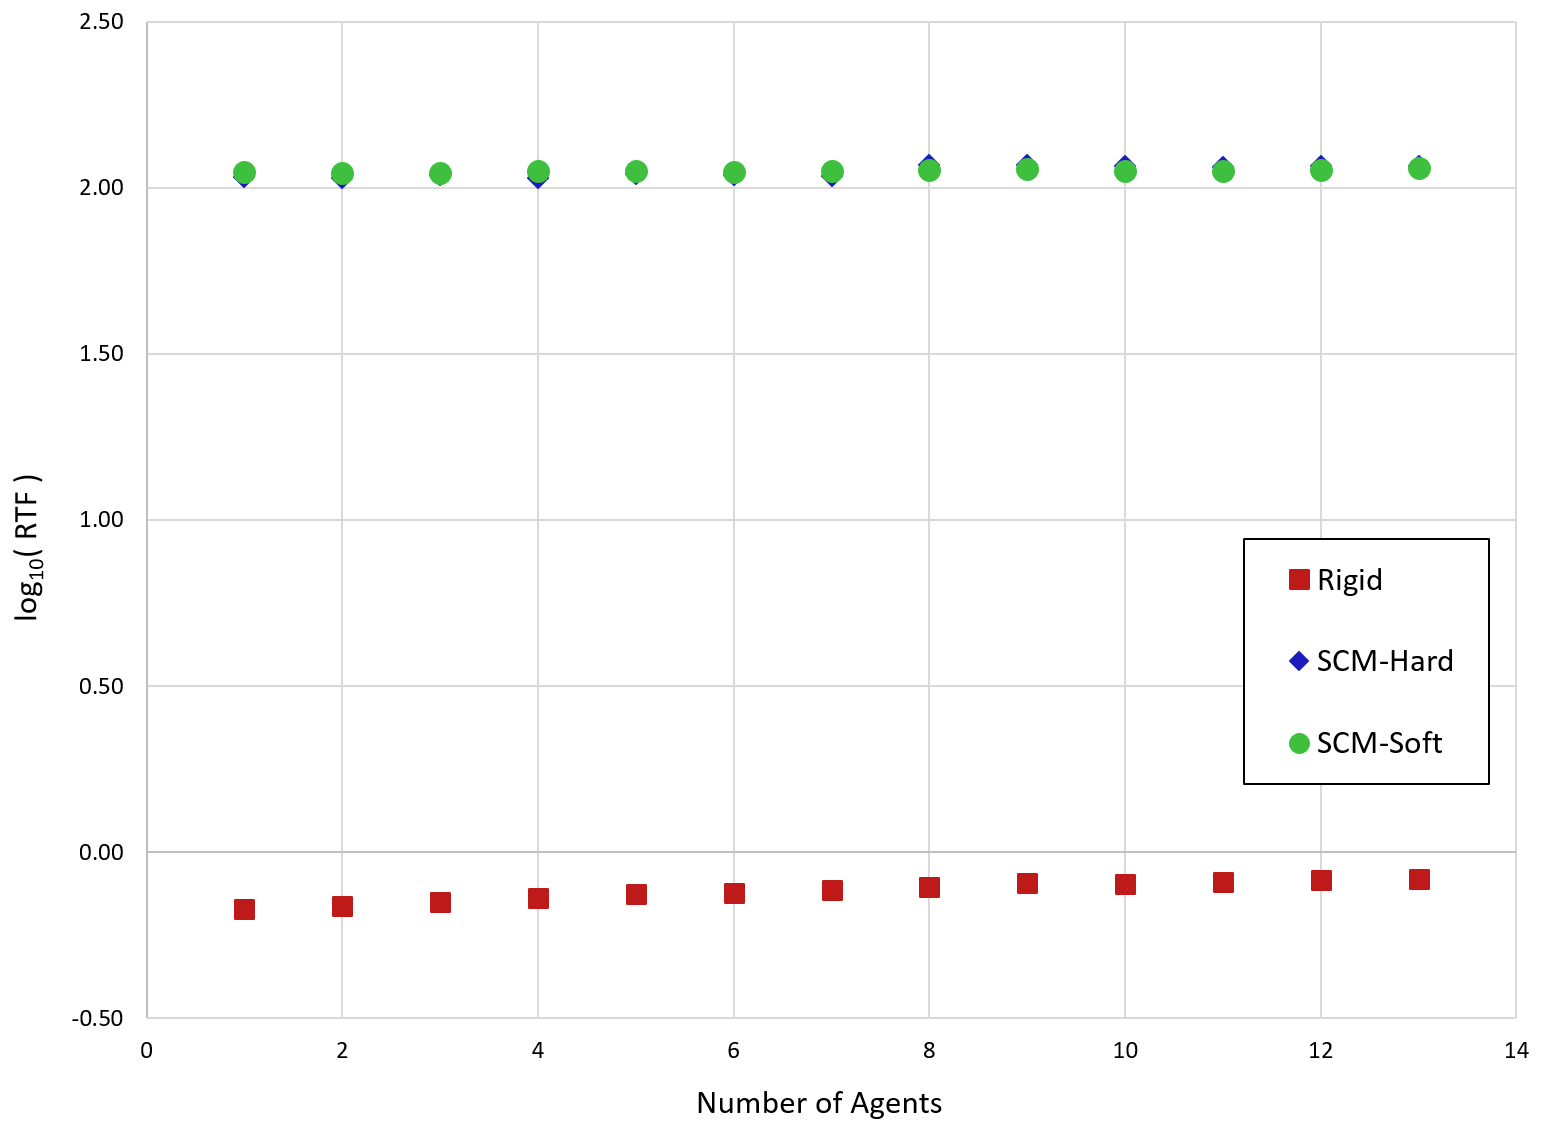
\includegraphics[width=\columnwidth]{Figs/syn_SCM_scaling.png}
    \caption{\synchrono{} scaling analysis for rigid, SCM hard, and SCM soft terrains. Logarithmic scale used.}   
    \label{fig:scmscaling}
\end{figure}

\begin{figure}
    \centering
    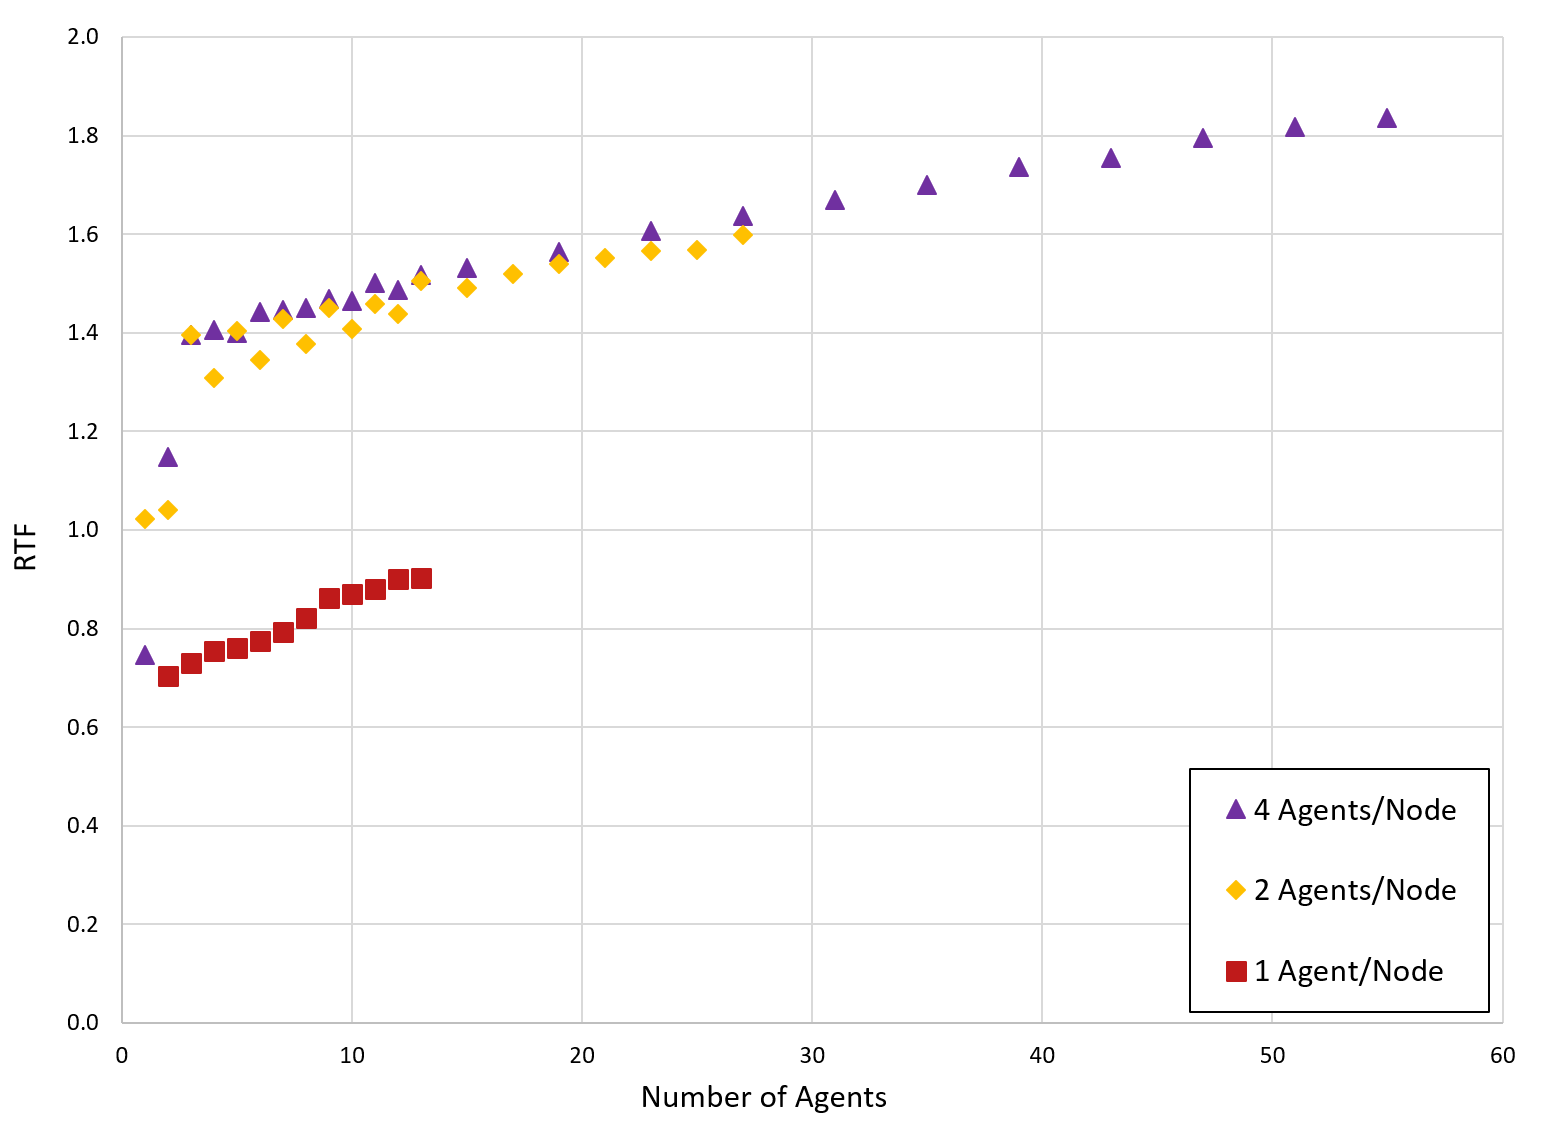
\includegraphics[width=\columnwidth]{Figs/syn_SCM_many.png}
    \caption{\synchrono{} scaling analysis on rigid terrain for a large number of agents.}   
    \label{fig:scmscalingrigid}
\end{figure}

%%\FloatBarrier

%%%%%%%%%%%%%%%%%%%%%%%%%%%%%%%%%%%%%%%%%%%%%%%%%%%%%%%%%%%%%%%%%%%%%%%%%%%%%%%%%%%%%%%%%%%%%%%% 
%%%%%%%%%%%%%%%%%%%%%%%%%%%%%%  LEARNING EXAMPLE  %%%%%%%%%%%%%%%%%%%%%%%%%%%%%%%%%%%%%%%%%%%%%% 
%%%%%%%%%%%%%%%%%%%%%%%%%%%%%%%%%%%%%%%%%%%%%%%%%%%%%%%%%%%%%%%%%%%%%%%%%%%%%%%%%%%%%%%%%%%%%%%% 
\subsection{Learning to drive in a convoy}
\label{subsec:learningDemo}


%{\SBELcomment{We should make it clear what the vehicles know, sense, communicate, etc. I don't think we do justice to this at this point.}}
%  

Chrono helps with two tasks: learning a control policy, and testing a policy that was designed in Chrono or brought from outside. In this example, PyChrono and GymChrono are used to design a policy. SynChrono is subsequently used to test it. The RL-based learning is done on rigid terrain using a nondescript texture. The goal is to enable a vehicle to move as part of a convoy. To test it, the policy is deployed on vehicles that are part of a four-vehicle convoy driving on rigid or SCM deformable terrain. Up to three of the convoy vehicles use this policy while driving in a platoon. Thus, the possible scenarios are: three lead vehicles and one following vehicle (3L+1F), two lead and two followers (2L+2F), and one lead and three followers (1L+3F). The \textit{lead} vehicles are programmed to follow a path defined by way-points; for all purposes, these can be considered human driven. A follower vehicle is autonomous and uses the learned policy to follow the vehicle in front of it. In doing so, it should not crash in the vehicle ahead of it, and avoid hitting obstacles in the vicinity of the path. To this end, it relis on a camera sensor, location acquired through GPS sensing, and compass heading. Note that communication allows a vehicle to find out the GPS location and velocity of the vehicle in front. Given that four vehicles are involved in this platooning experiment, SynChrono is subsequently used to test the policy to reduce simulation times. Indeed, this validation could be run in Chrono::Engine but would roughly require four times longer to complete it. The salient points of this experiment are as follows: although vehicles are run in different SynChrono processes, there is time and space coherence between them to the point where the vehicles sense each other; the learning occurs using rigid terrain with nondescript texture but the policy is tested on deformable terrain that is white (snow-like); this is an end-to-end policy that uses sensor data fusion to control both the steering and acceleration/braking of the vehicle.

\paragraph{Designing a policy.} The policy was obtained through training using a custom implementation of the PPO reinforcement learning algorithm leveraging PyTorch~\cite{paszke2017PyTorch} as the Deep Learning framework. The agent is a HMMWV vehicle modeled in Chrono::Vehicle. The goal of the training process is to develop a control policy that enables an agent (in this case the HMMWV) to drive in a convoy. For training, to increase the randomness of the path and thus the robustness of the control, two different path types were used on a 90x90 meters area. The first is S-shaped, starting from a corner and finishing in the opposite corner; the second is C-shaped, starting and finishing on the same side of the driving area. To further increase the randomness, these paths can be flipped along the $y$-axis (left-right) and rotated about the vertical $z$-axis to obtain 16 different possible paths. The starting point is picked randomly within the first half of the path as shown in Fig.~\ref{fig:paths}. Eight obstacles placed near the path are randomly selected from various rock, tree, and bush assets. 

%\todo[inline]{SB: Two options, pick your favorite.}
%\begin{figure}
%    \centering
%    \includegraphics[width=\columnwidth]{Figs/all_paths.pdf}
%    \caption{All possible paths. The dashed lines represent the segment of the path in which the simulation episode can start}   
%    \label{fig:paths_all}
%\end{figure}

\begin{figure}
    \centering
    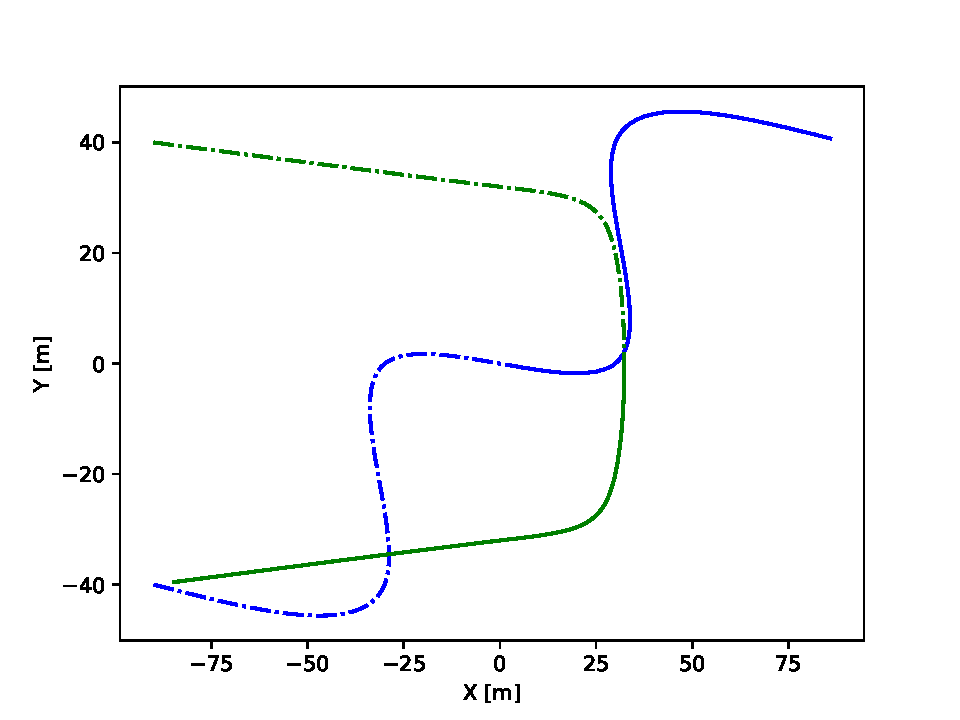
\includegraphics[width=\columnwidth]{Figs/base_paths.pdf} 
    \caption{The double S and C paths used during training. Each one of these is randomly flipped and rotated, resulting in 16 different possible paths. The dashed lines represent the segment of the path in which the simulation episode can start.}
    \label{fig:paths}
\end{figure}

In order for the agent to accomplish its task, the vehicle must be aware of its surroundings. To that end, the HMMWV used two sensors simulated in Chrono::Sensor: a GPS sensor, and an RGB camera placed on the front bumper. The camera, which updates at 30 Hz, has a resolution of 80 $\times$ 45 pixels. This level of resolution suffices, since detailed features that can be extracted from higher resolution images are not needed by the control policy. Furthermore, given that the dataset contains one image per interaction, images of too high resolution can quickly deplete the available GPU memory due to the increased memory footprint of the NN update process. As such, large images that are contained in observations are typically avoided. 

As with any other RL environment, an observation and a reward is provided to the ML algorithm at each timestep. Subsequently, the agent must perform an action prescribed by the ML algorithm in order to maximize the reward collected. The action is a two element array: the first is a steering value; the second element is a combined throttling and braking value. The choice of collapsing throttle and brake control into the same action was taken to avoid simultaneous braking and throttling and because throttling and braking both directly control the vehicle's acceleration. 

The agent is rewarded only when it successfully stays behind the leader, meaning a reward is provided when the angle between the heading of the leader and the follower is in the range $[-\pi/4, \pi/4]$. When this condition is met, the agent receives the maximum reward if it keeps an optimal distance (within a prescribed tolerance) from the lead vehicle. In other words, the follower is rewarded when it stays in a sector of an annulus centered at the leader. When the vehicle is outside the desired area, the reward decreases hyperbolically. 
\begin{figure*}
    \centering
    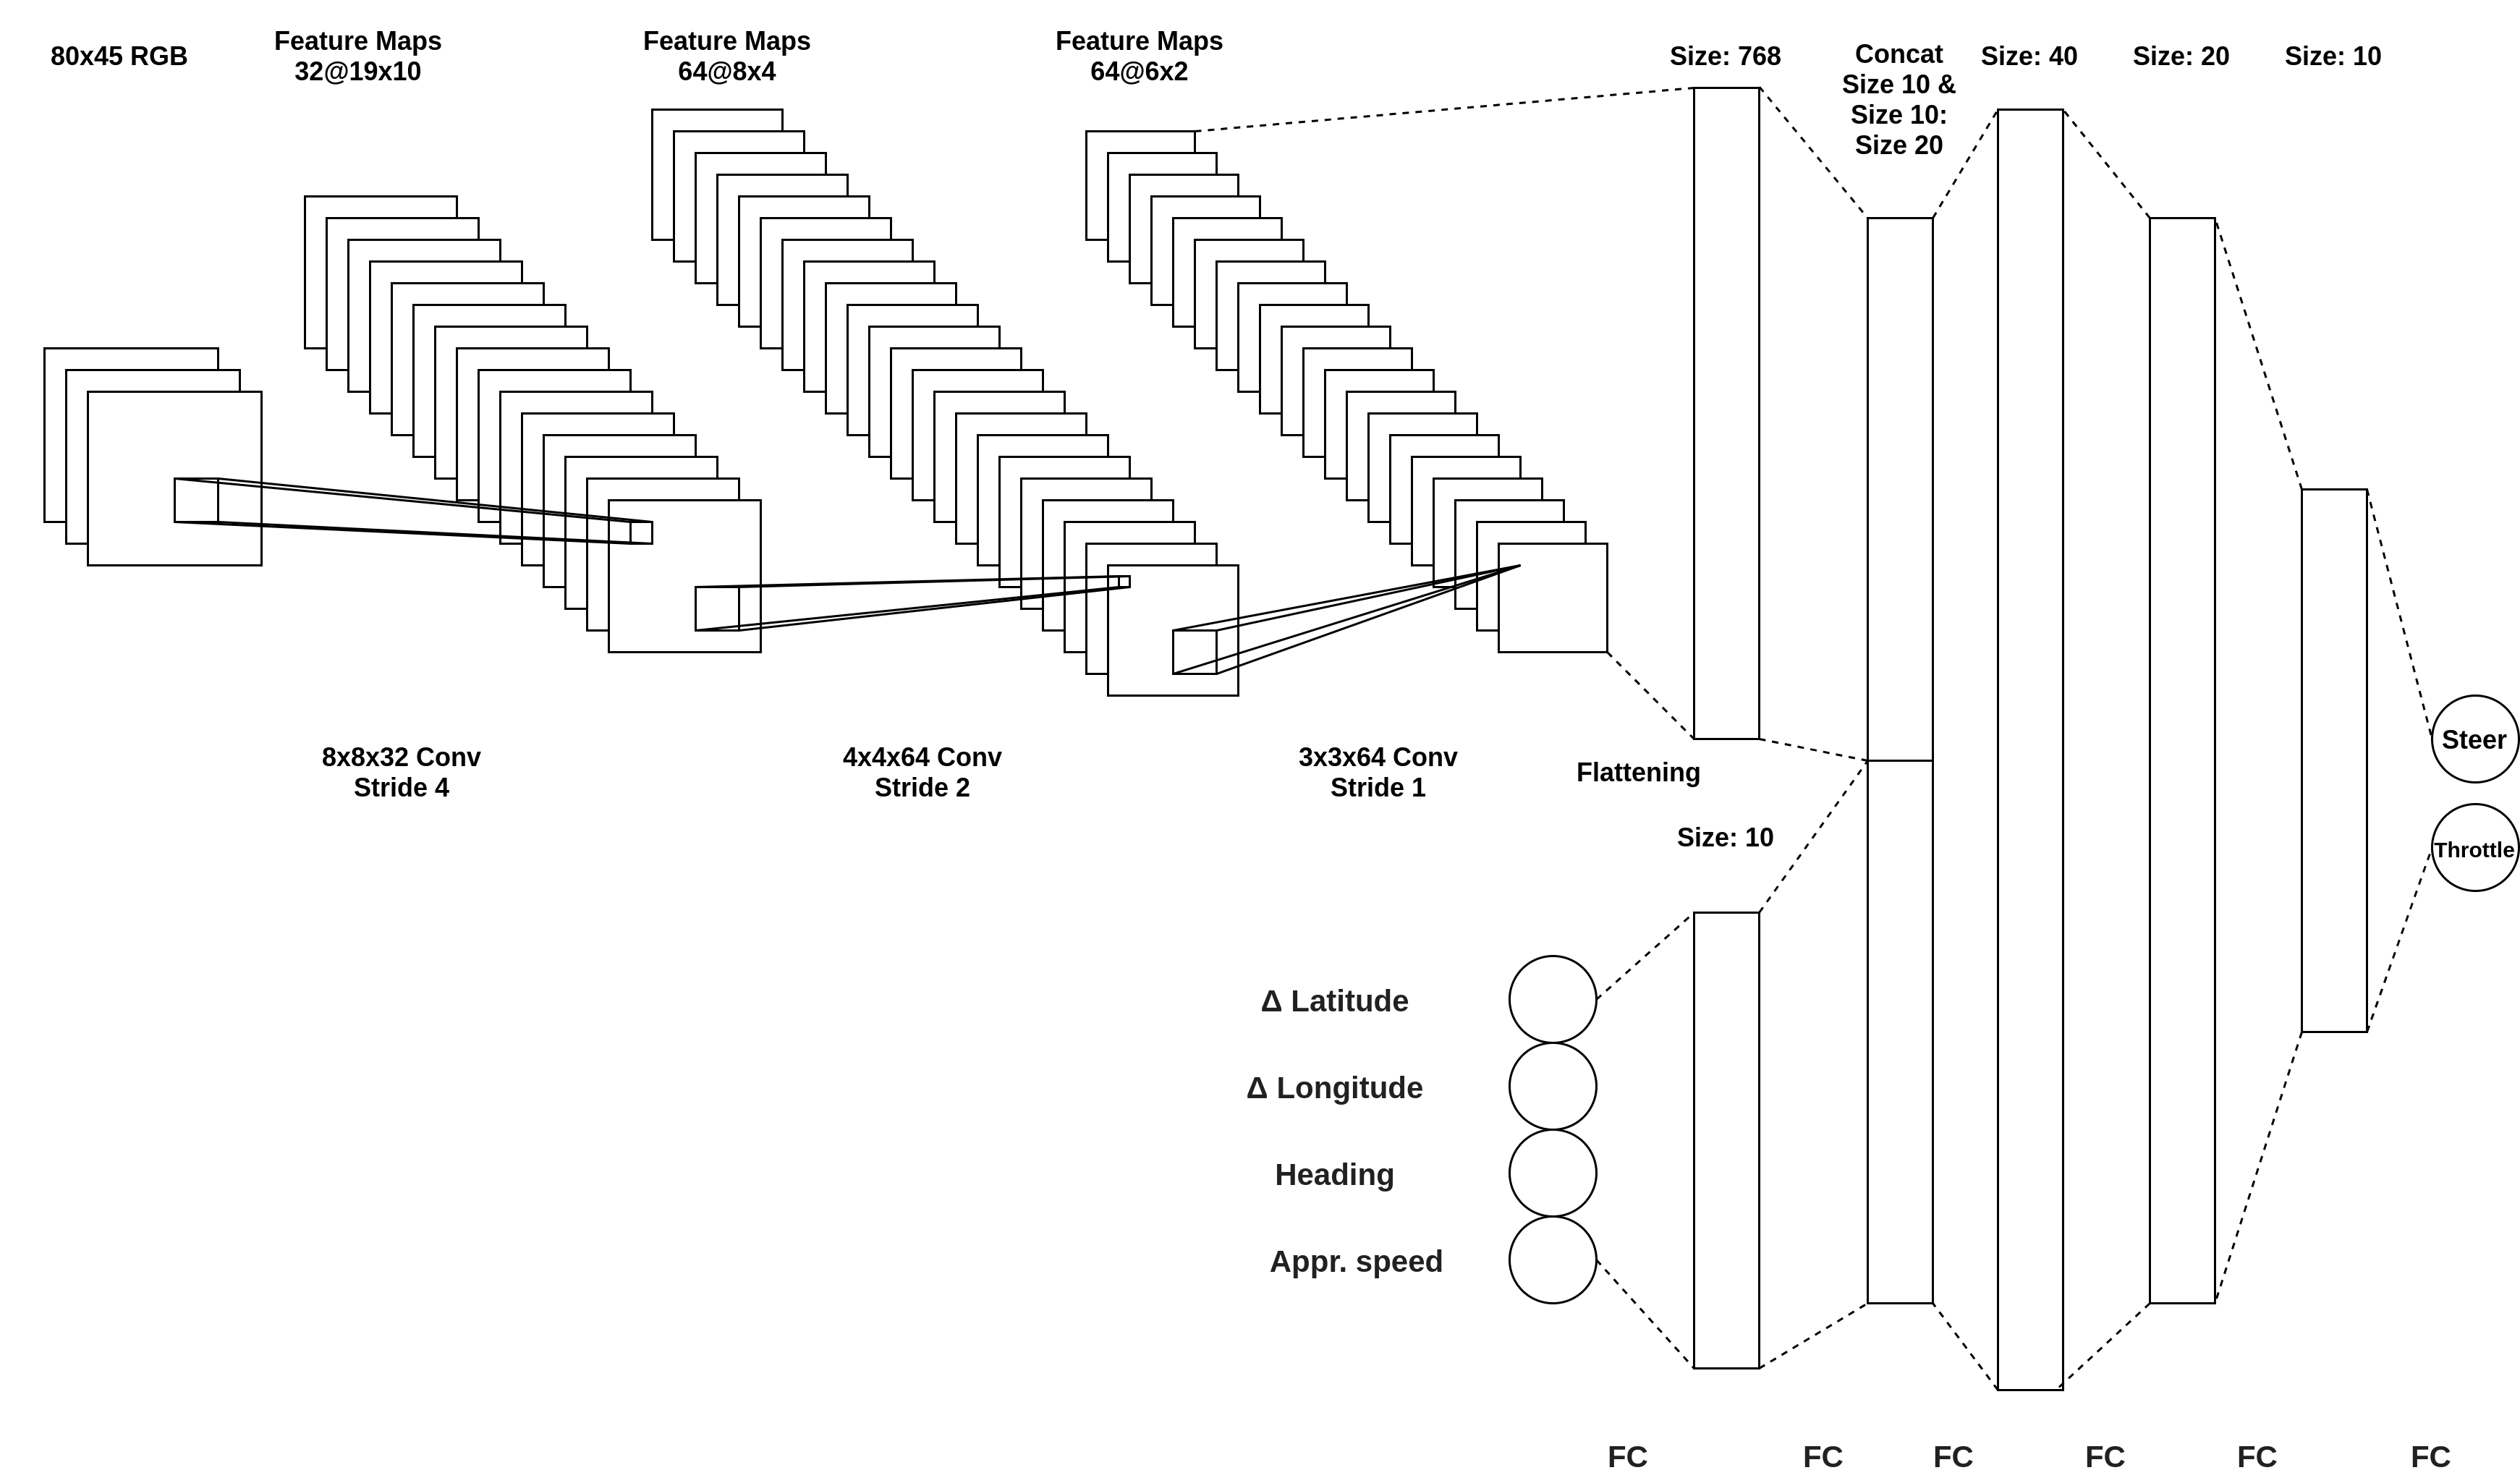
\includegraphics[angle=90,width=0.6\linewidth]{Figs/MS_NN.png}
    \caption{{\small Sensor Fusion NN architecture.}}   
    \label{fig:NNarch}
\end{figure*}

The learning draws on information from several sensors, whose output is organized into two tuples. The first element is a 80 $\times$ 45 $\times$ 3 RGB image. The second is a vector of four values: the latitude and longitude difference between the leader and the follower; the heading according to the compass; and the speed at which the follower is approaching the leader. This multi-sensor observation required the NN architecture to incorporate an input composed of a 3D and a 1D tensor. The image is processed in a Convolutional Neural Network (CNN) as in~\cite{Mnih13}. Its output is then concatenated with the output of the one Fully Connected (FC) hidden layer Deep Neural Network (DNN) which takes the 1D Tensor as input. Their concatenated output is then processed by three FC hidden layers. The architecture of the model is shown in Fig.~\ref{fig:NNarch}.

RL-based training requires a very large number of iterations. Three decisions helped speed up the learning process: ($i$) the lead vehicles were not simulated, but only rendered at the correct location and orientation (as this has no bearing for sensing purposes); ($ii$) a reduced-order model of the HMMWV vehicle was used in the first stage of training, with the more computationally demanding full vehicle model substituted during the training process (see Fig.~\ref{fig:Rewards}) to further refine the NN parameters; and ($iii$) the learning process was accelerated using the OpenAI~\cite{Brockman16Gym} Baselines tool for environment parallelization, thus allowing several simulations running simultaneously to speed up the collection of the dataset samples.

%{\SBELcomment{NOTE: In the caption for Fig.~\ref{fig:Rewards} we talk about things that we don't touch upon in the text. Caption is hard to understand (except switching to full vehicle -- we do touch on this in the text).}} {\SBELcomment{SB: I got rid of some unnecessary details}}

\begin{figure}
	\centering
	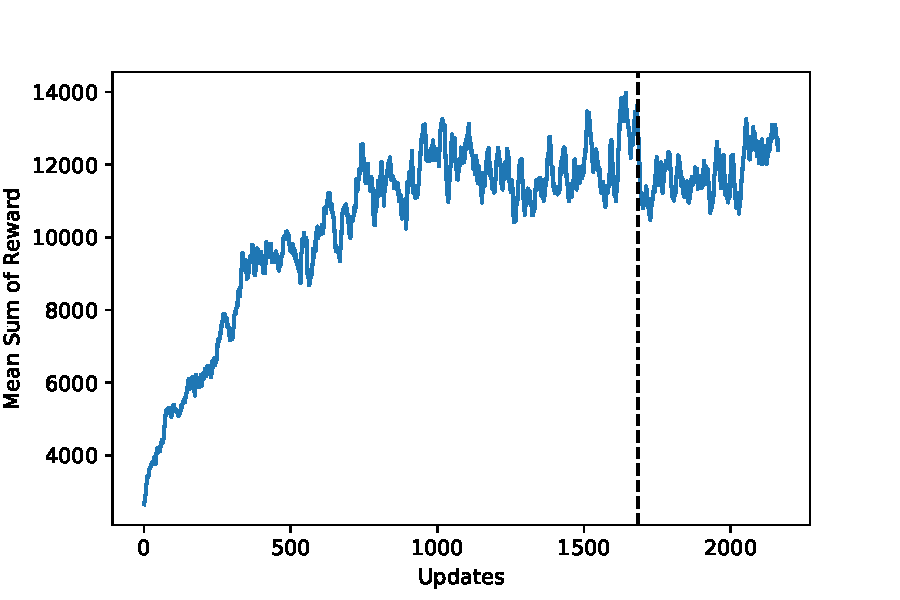
\includegraphics[width=\columnwidth]{Figs/rewards.pdf}
	\caption{Plot of the moving average of the sum of collected rewards with respect to the policy updates (updated every 1500 interactions). The vertical dashed line represents the switch from the reduced to the full HMMWV model.}
	\label{fig:Rewards}
\end{figure}


\paragraph{Testing of learned policy.}  The AA control policy derived in PyChrono and GymChrono was tested in SynChrono for various convoy setups while operating on three terrain types. The platoons were 3L+1F, 2L+2F, and 1L+3F. The terrains were rigid, SCM hard (silt-like), and SCM soft (snow-like). This leads to a set of nine platooning scenarios. In the following discussion, the leader and follower vehicles are numbered starting from the head of the convoy; for example, the order of the vehicles in a 1L+3F configuration is: Leader, Follower 1, Follower 2, Follower 3.

For each platooning scenario, data recorded from simulations included position, velocity, and acceleration for each of the four vehicles. In addition, a high definition camera sensor was attached to the last vehicle in the convoy in order to visualize the simulation. Still frames captured with this camera are shown in Fig.~\ref{fig:simscreenshots} and full-length videos of representative simulations are available online~\cite{simsPaperGVSETS2020}. Different ground textures and colors were used to further differentiate between the three terrain types (rigid, SCM-Hard, and SCM-Soft).
%
\begin{figure*}
    \centering
    \begin{subfigure}{0.33\textwidth}
        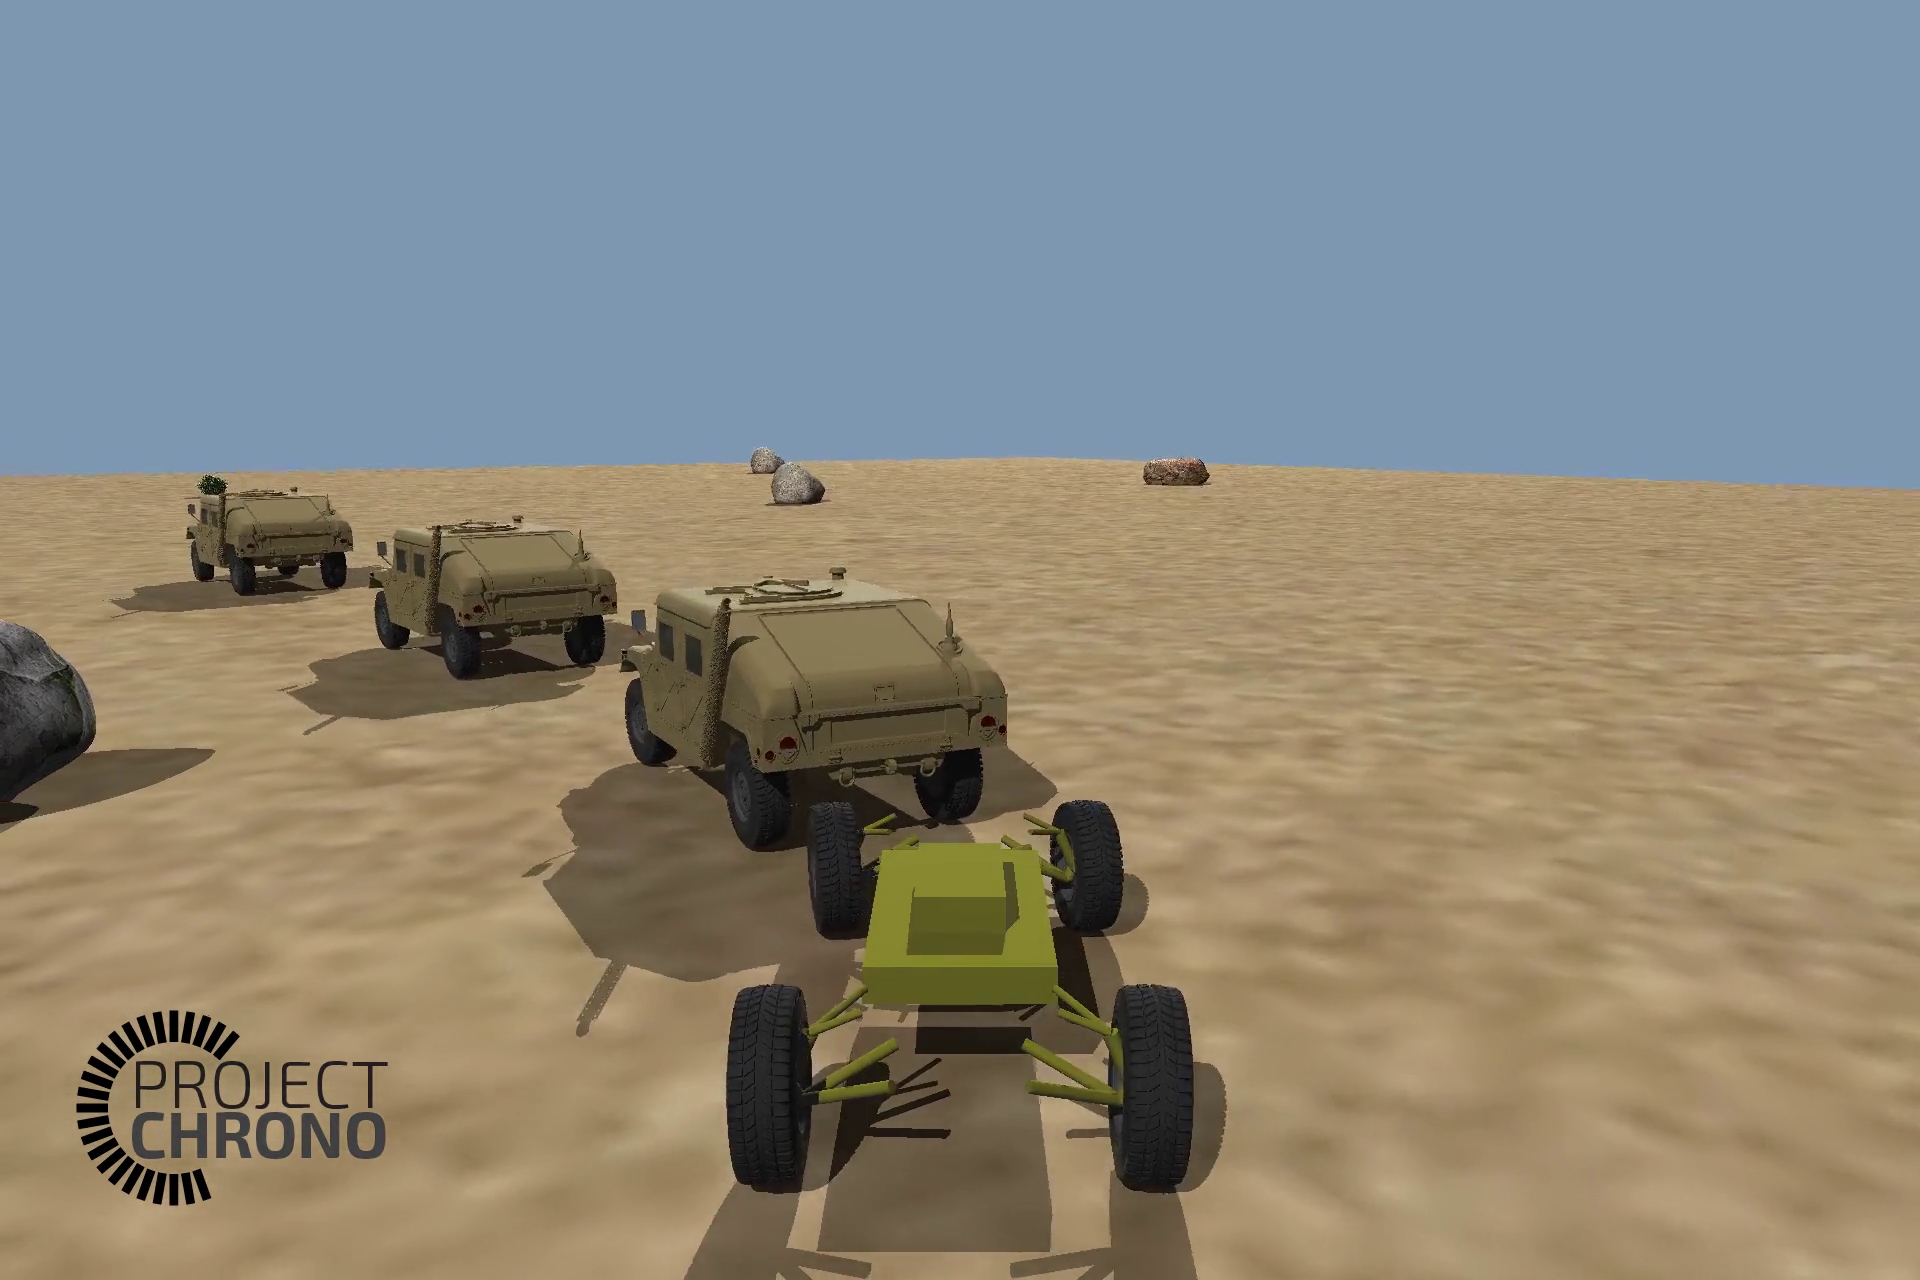
\includegraphics[width=\linewidth]{Figs/Demonstration/rigid_1i_3f.png}
        \caption{} \label{fig:rigid13}
    \end{subfigure}%
    \begin{subfigure}{0.33\textwidth}
        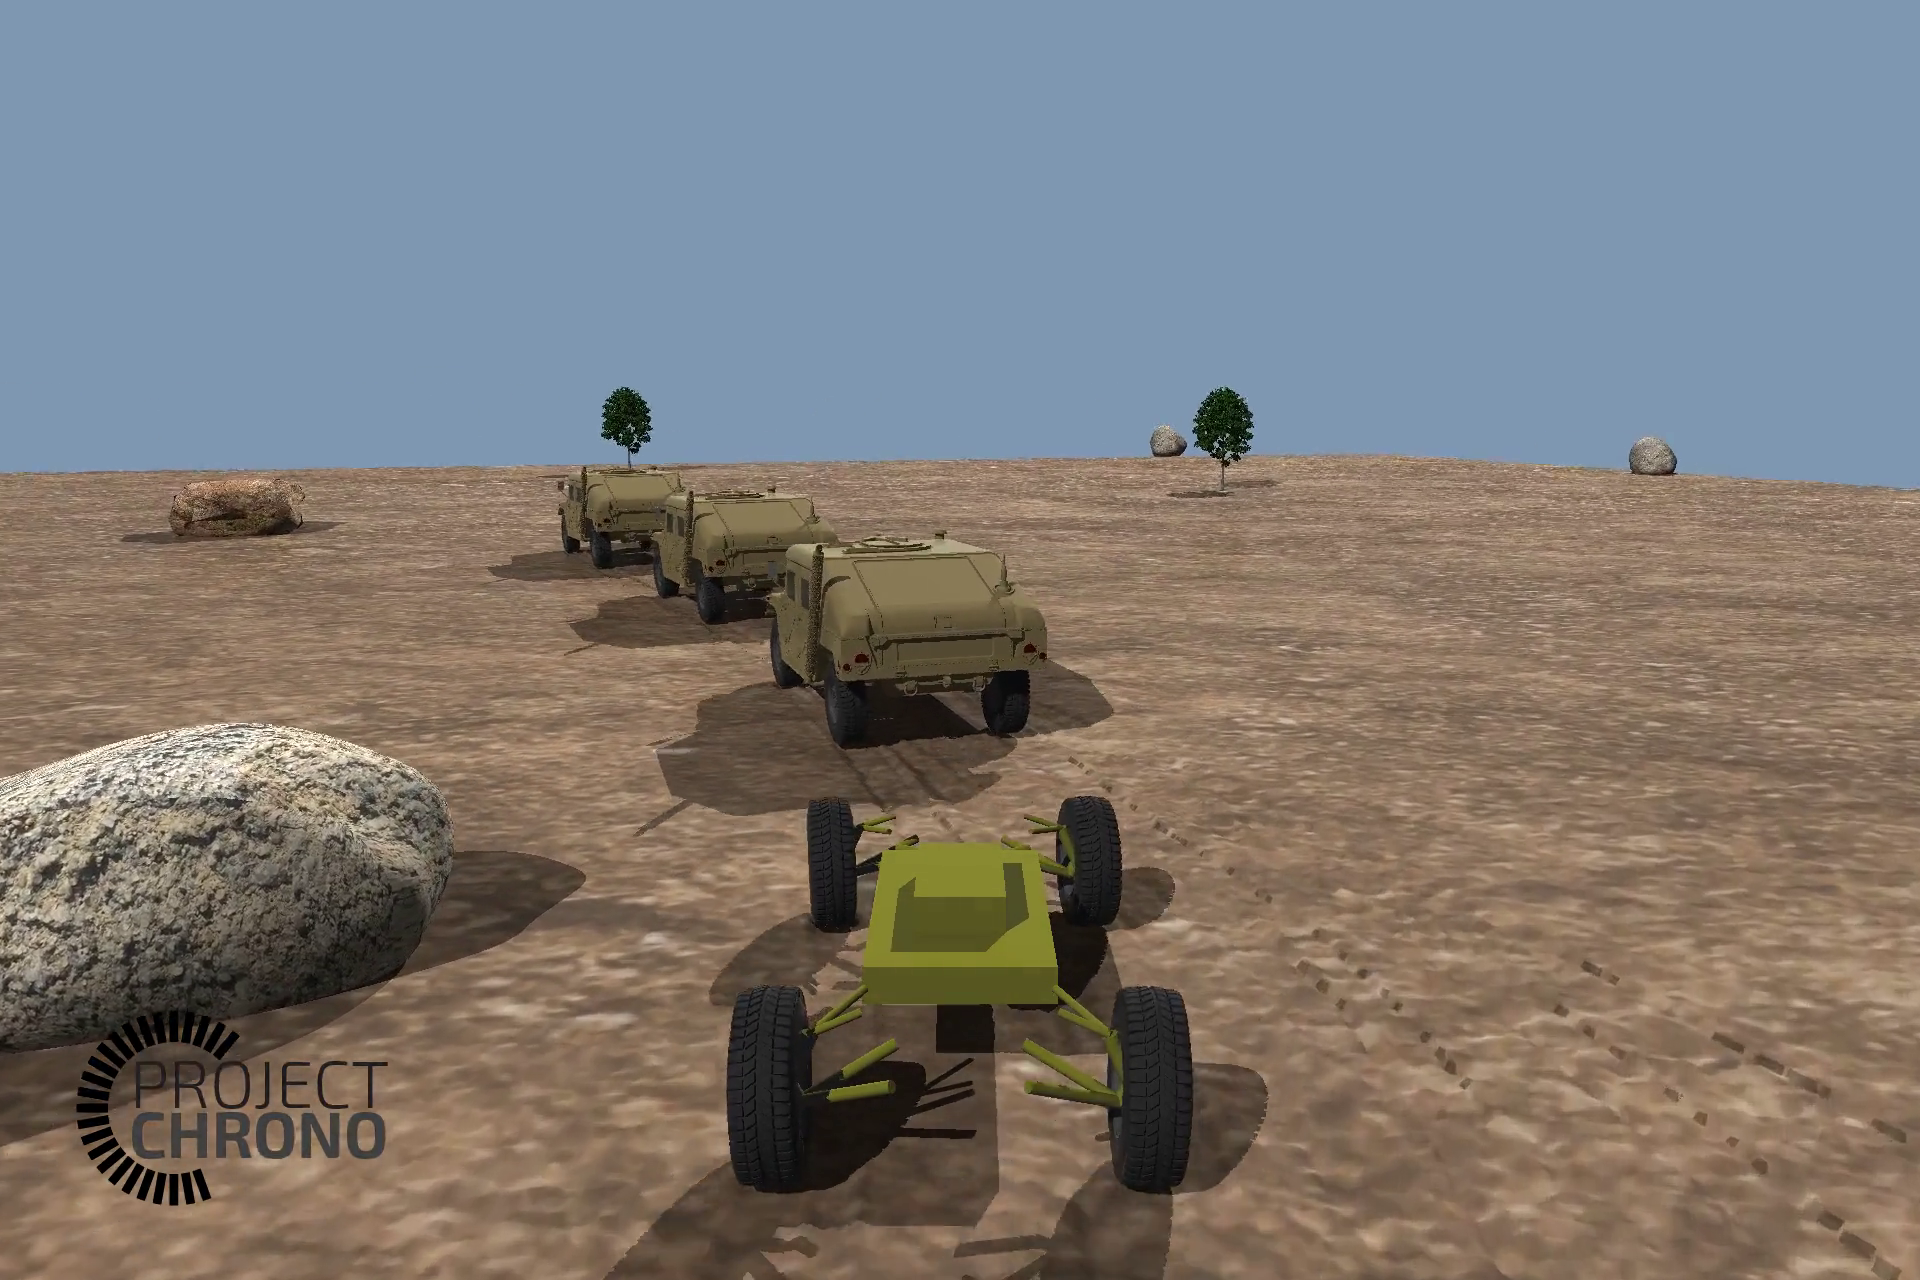
\includegraphics[width=\linewidth]{Figs/Demonstration/hard_1i_3f.png}
        \caption{} \label{fig:hard13}
    \end{subfigure}%
    \begin{subfigure}{0.33\textwidth}
        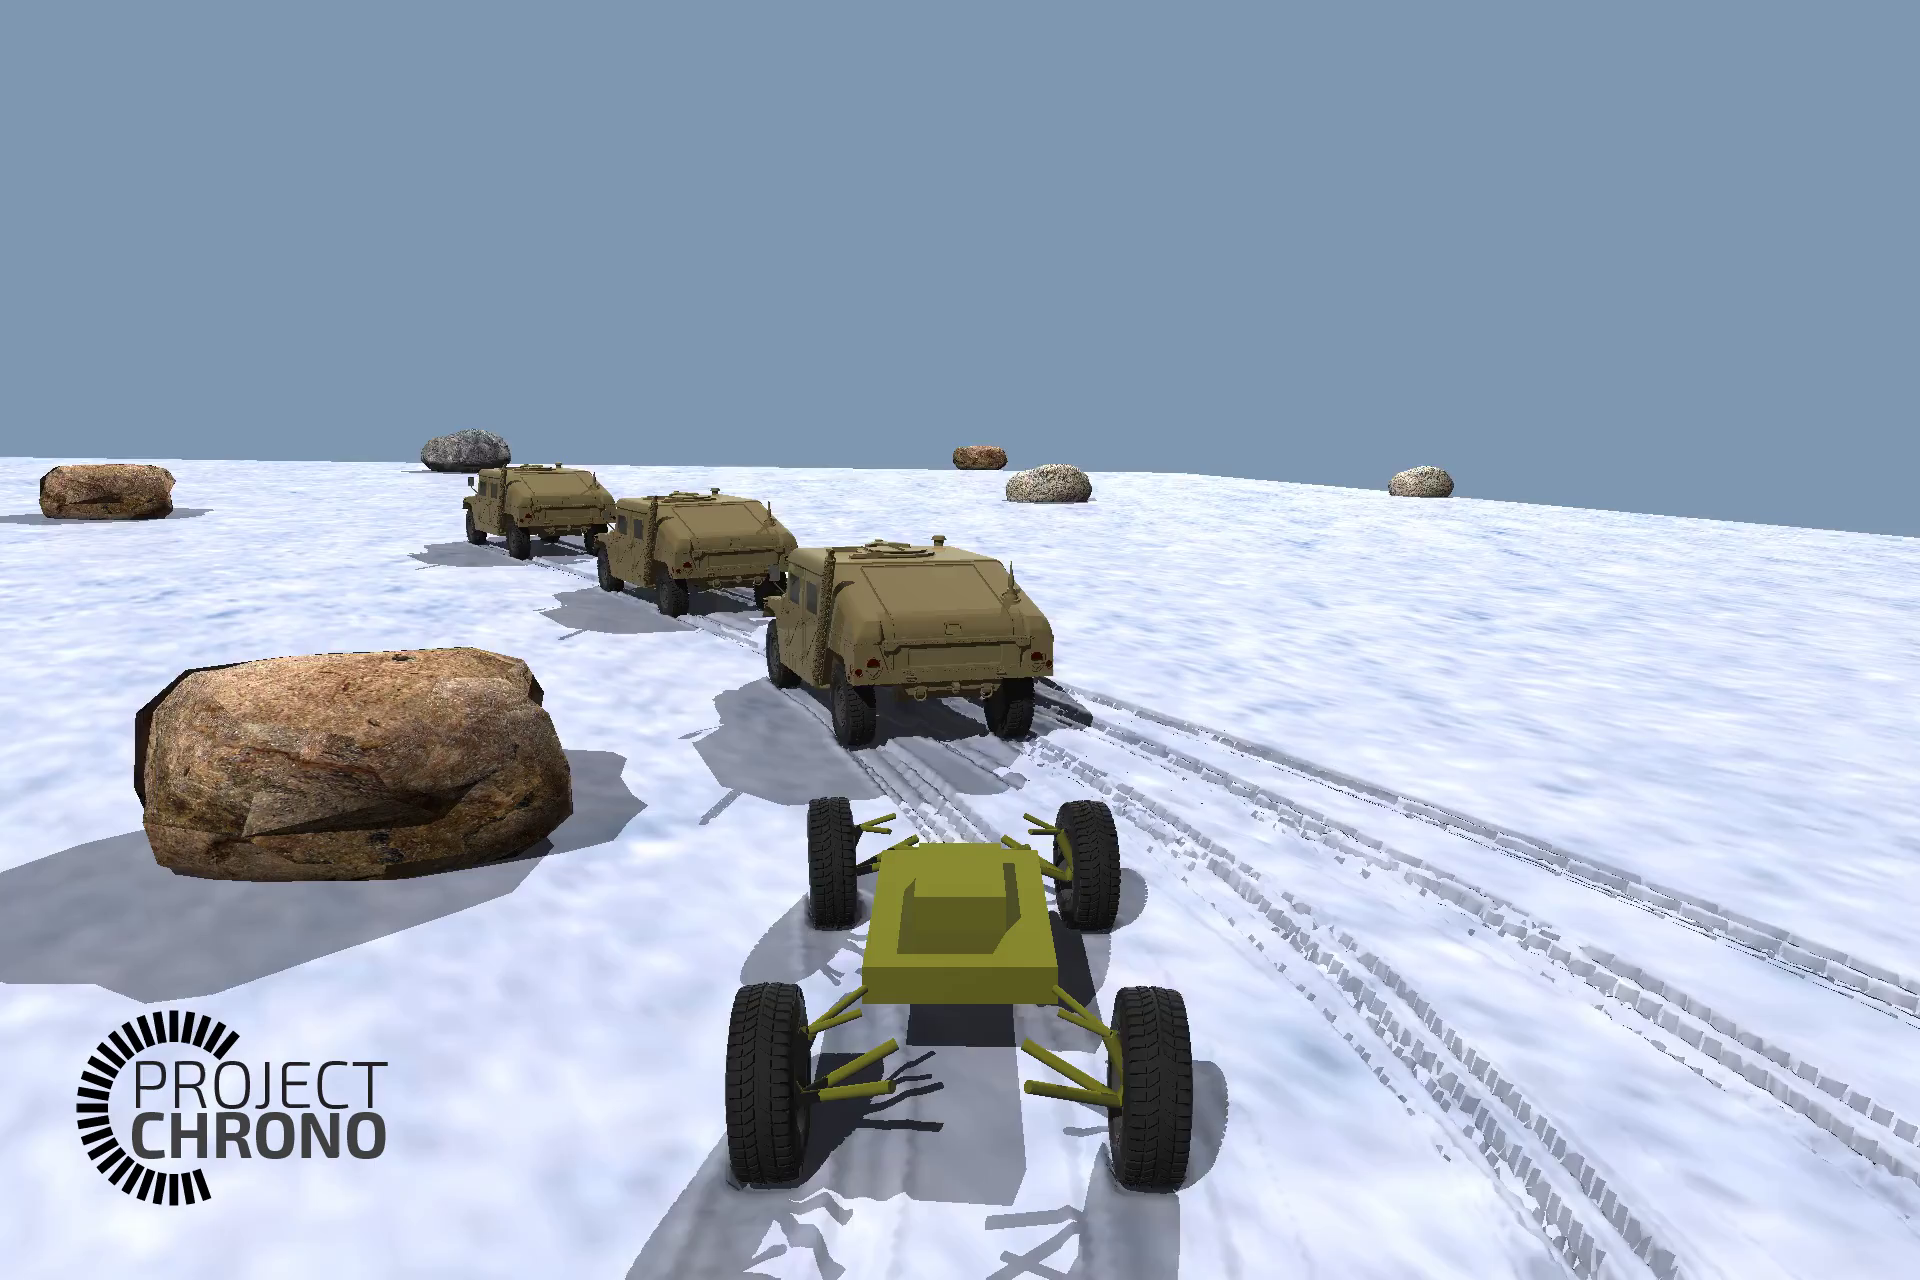
\includegraphics[width=\linewidth]{Figs/Demonstration/soft_1i_3f.png}
        \caption{} \label{fig:soft13}
    \end{subfigure}%
    \caption{Still frames from attached third person camera: (a) rigid terrain; (b) SCM-Hard terrain; (c) SCM-Soft terrain.}   
    \label{fig:simscreenshots}
\end{figure*}

Table~\ref{tab:vehiclepositions} shows top-down views of the convoy trajectories for each platooning scenario, with solid and dashed lines representing leader and follower trajectories, respectively.
As these images indicate, different simulation configurations lead to different reactions of the follower vehicles. The training process described in \S\ref{subsec:learningDemo} rewards a follower vehicle for being within a certain angle and distance of the leader; as a result, this allows for deviations between the paths of follower and leader vehicles as well as deviations in the speed at which leader and follower vehicles negotiate a certain path segment.


%
\begin{table*}
    \centering
    \caption{2D Positions of each vehicle in each simulation configuration}
    \label{tab:vehiclepositions}
    \begin{tabular} { cccc }
         & \hspace*{.75cm}3L$ + $1F& \hspace*{.75cm}2L$ + $2F& \hspace*{.75cm}1L$ + $3F \\
        %\hline 
        %\\ 
        {\rotatebox[origin=c]{90}{Rigid}}&
        \parbox[c]{2.02in}{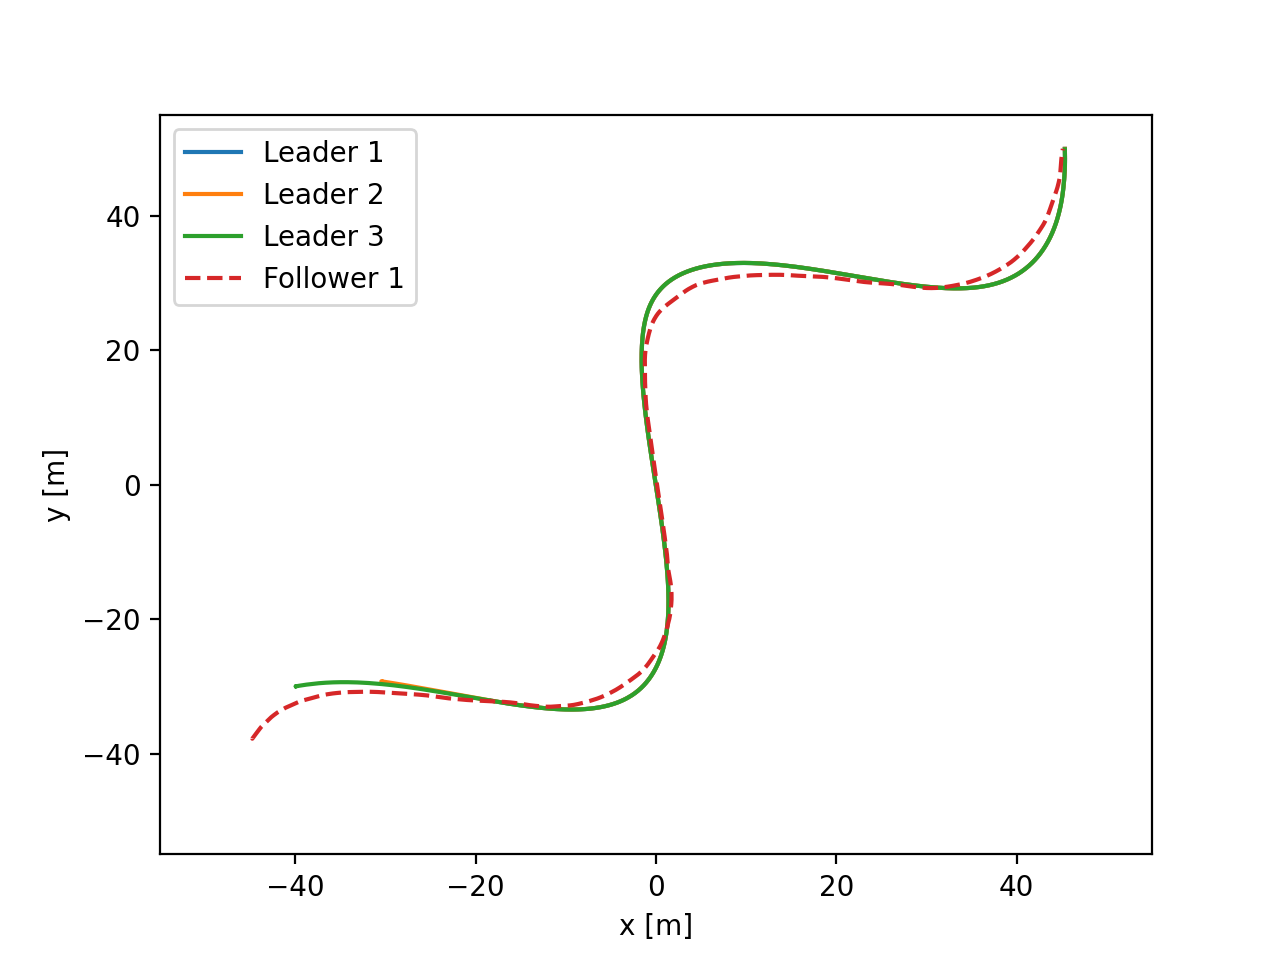
\includegraphics[height=1.8in]{Figs/Demonstration/3f_1i_rigid_positions.png}}&
        \parbox[c]{2.02in}{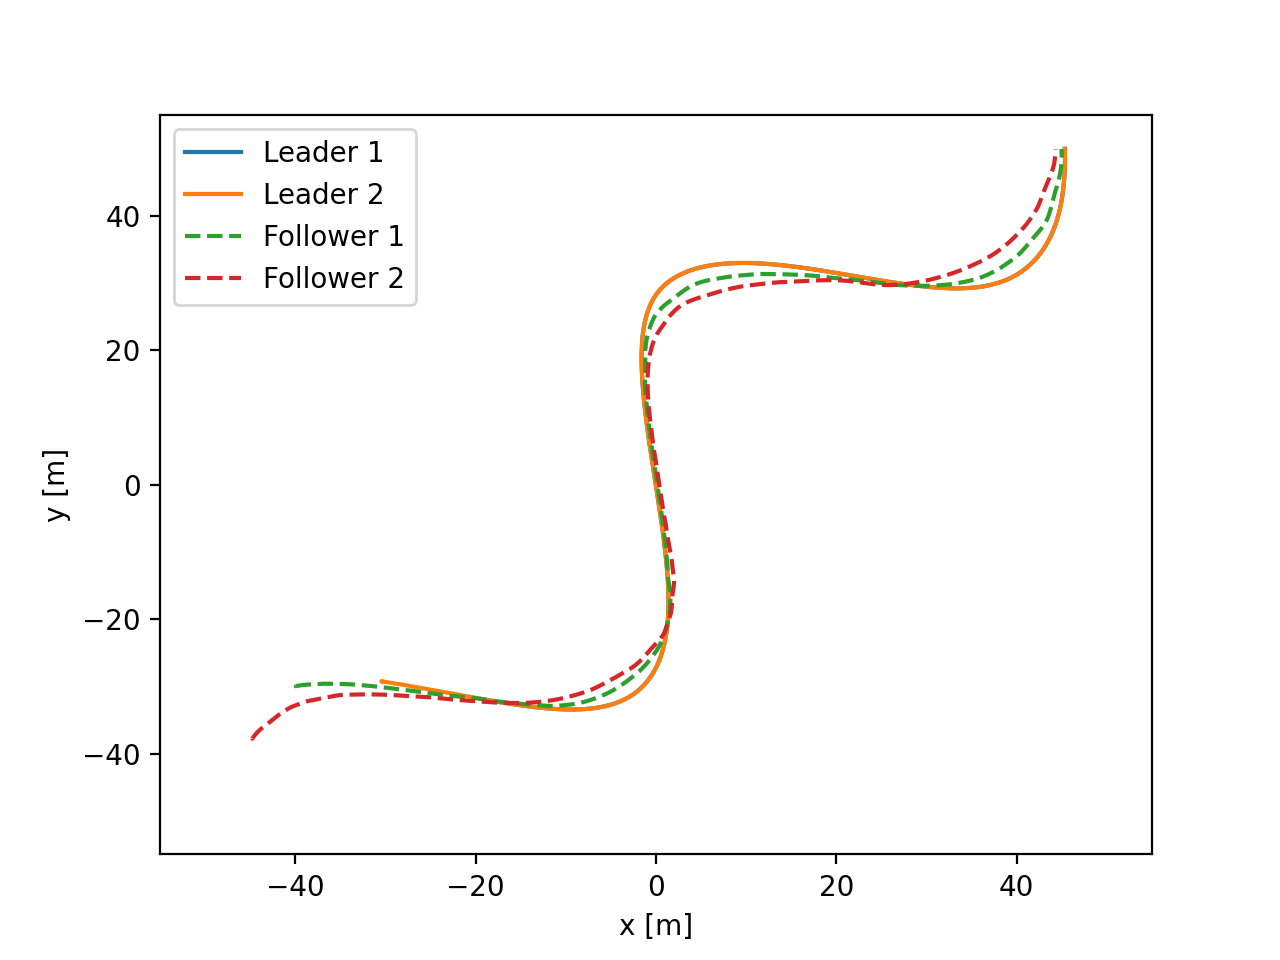
\includegraphics[height=1.8in]{Figs/Demonstration/2f_2i_rigid_positions.png}}&
        \parbox[c]{2.02in}{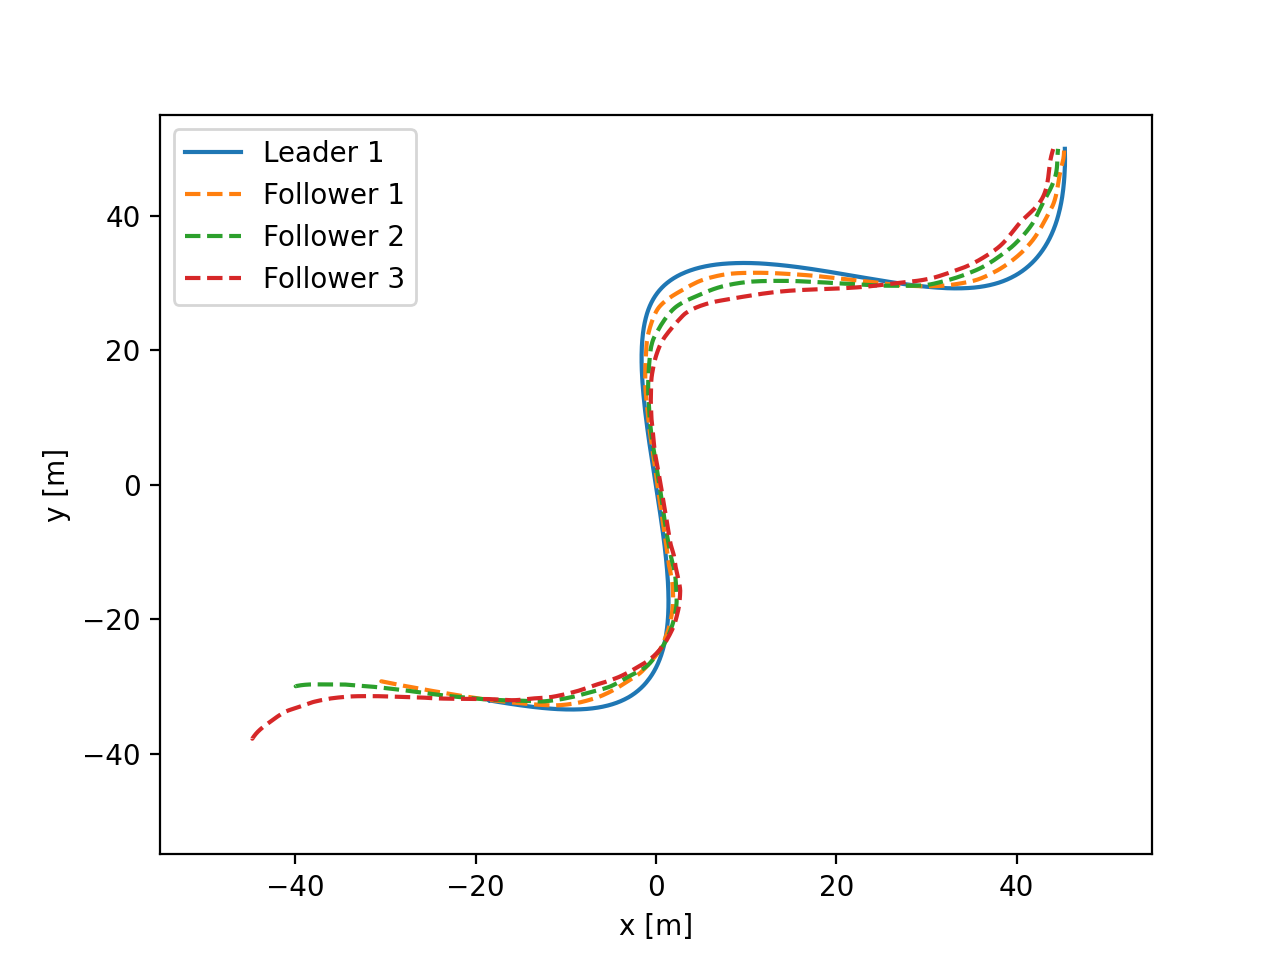
\includegraphics[height=1.8in]{Figs/Demonstration/1f_3i_rigid_positions.png}}\\
        %\newline \\
        %\hline 
        %\\ 
        {\rotatebox[origin=c]{90}{SCM-Hard}}&
        \parbox[c]{2.02in}{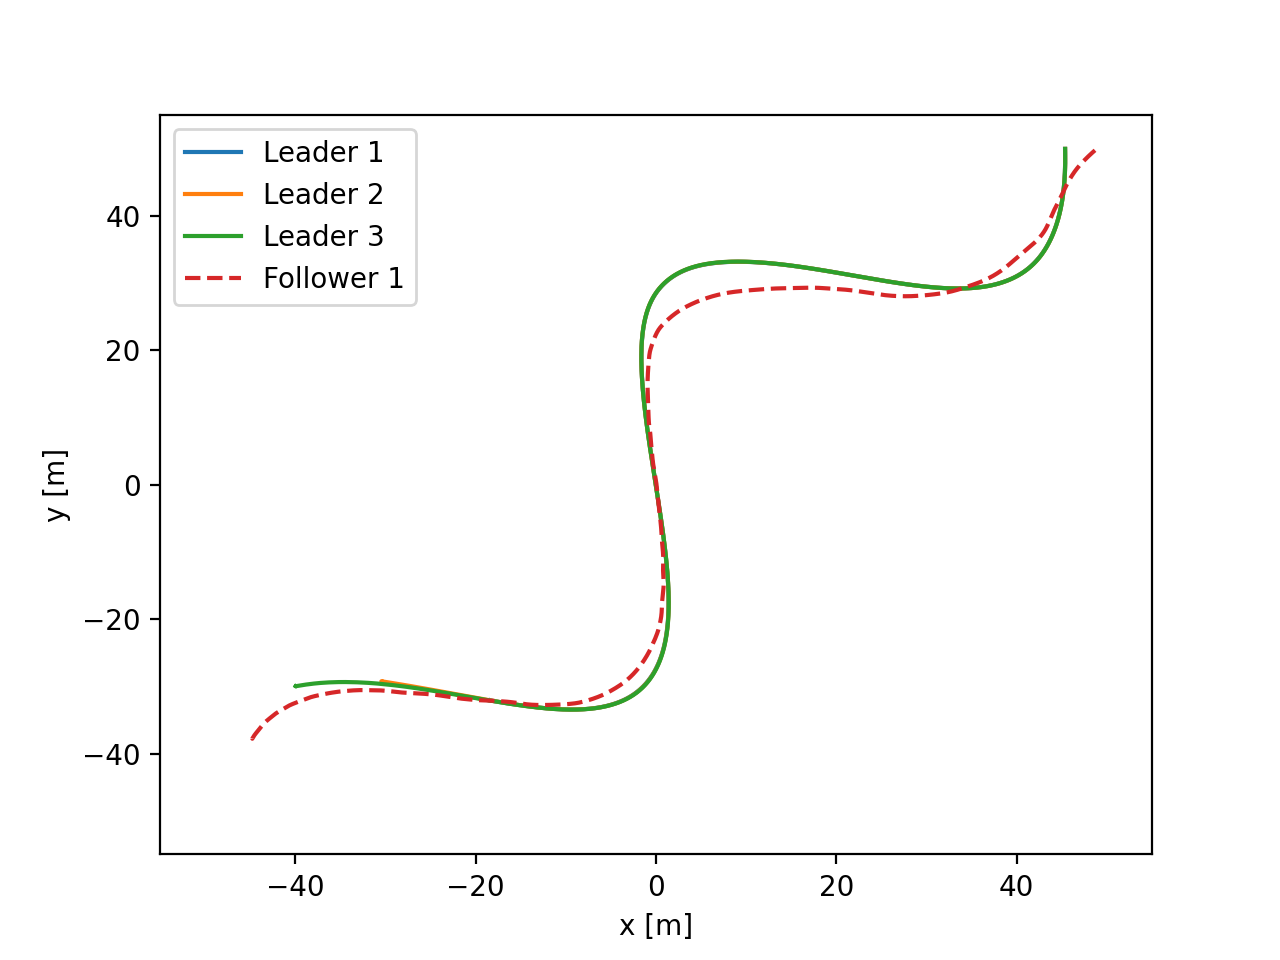
\includegraphics[height=1.8in]{Figs/Demonstration/3f_1i_hard_positions.png}}&
        \parbox[c]{2.02in}{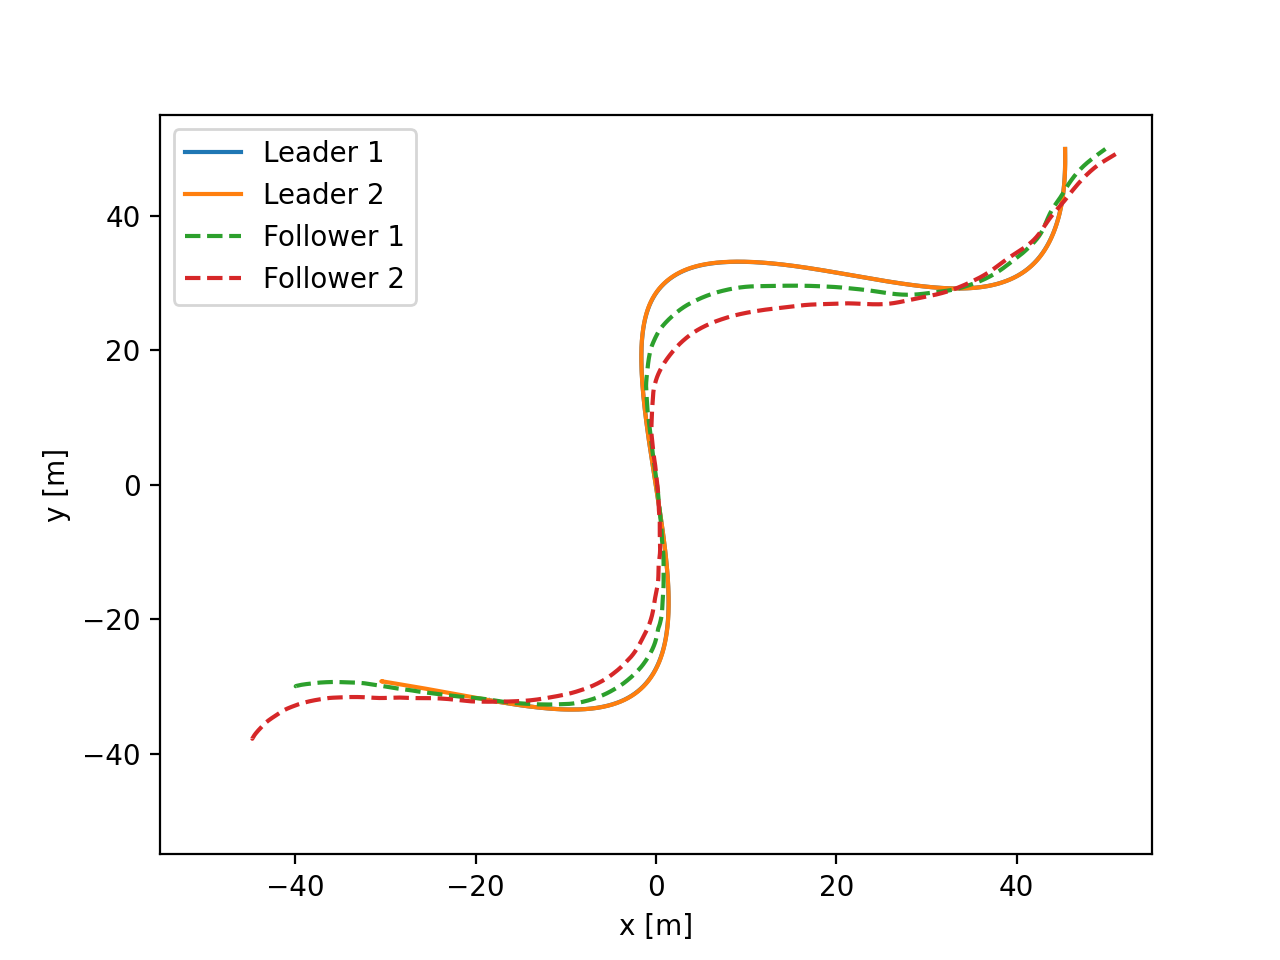
\includegraphics[height=1.8in]{Figs/Demonstration/2f_2i_hard_positions.png}}&
        \parbox[c]{2.02in}{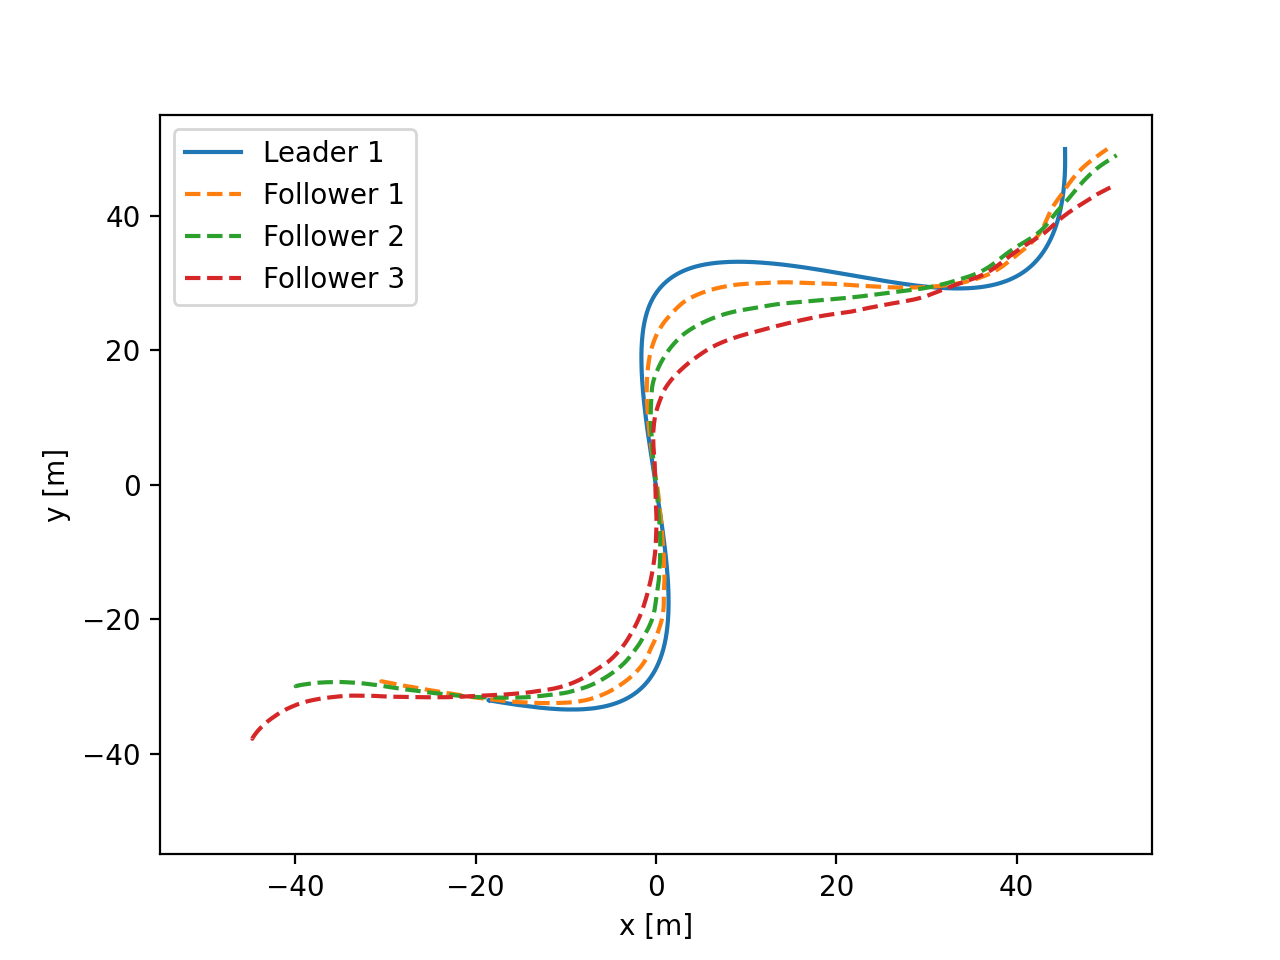
\includegraphics[height=1.8in]{Figs/Demonstration/1f_3i_hard_positions.png}}\\
        %\newline \\
        %\hline 
        %\\
        {\rotatebox[origin=c]{90}{SCM-Soft}}&
        \parbox[c]{2.02in}{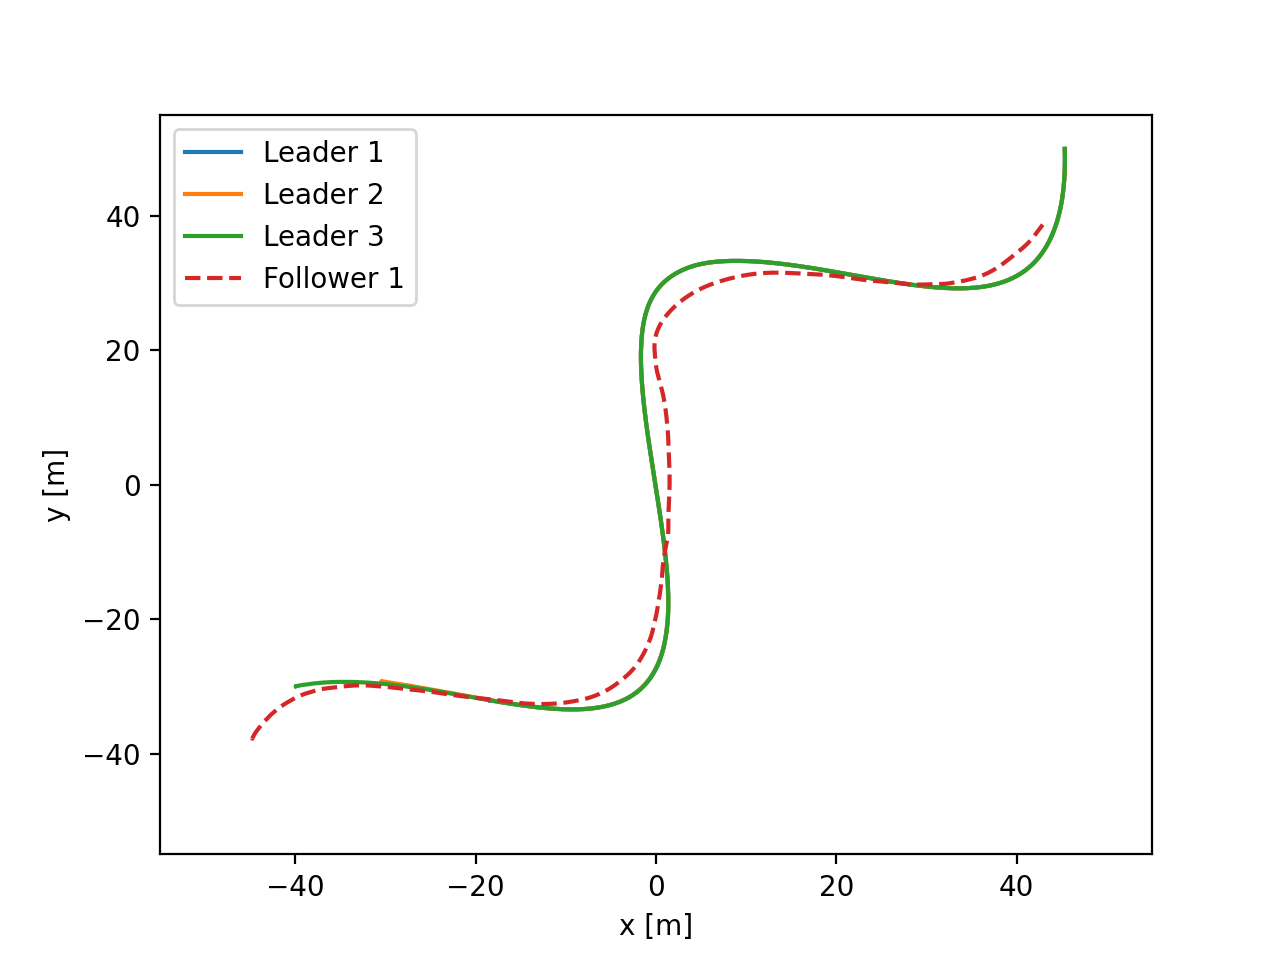
\includegraphics[height=1.8in]{Figs/Demonstration/3f_1i_soft_positions.png}}&
        \parbox[c]{2.02in}{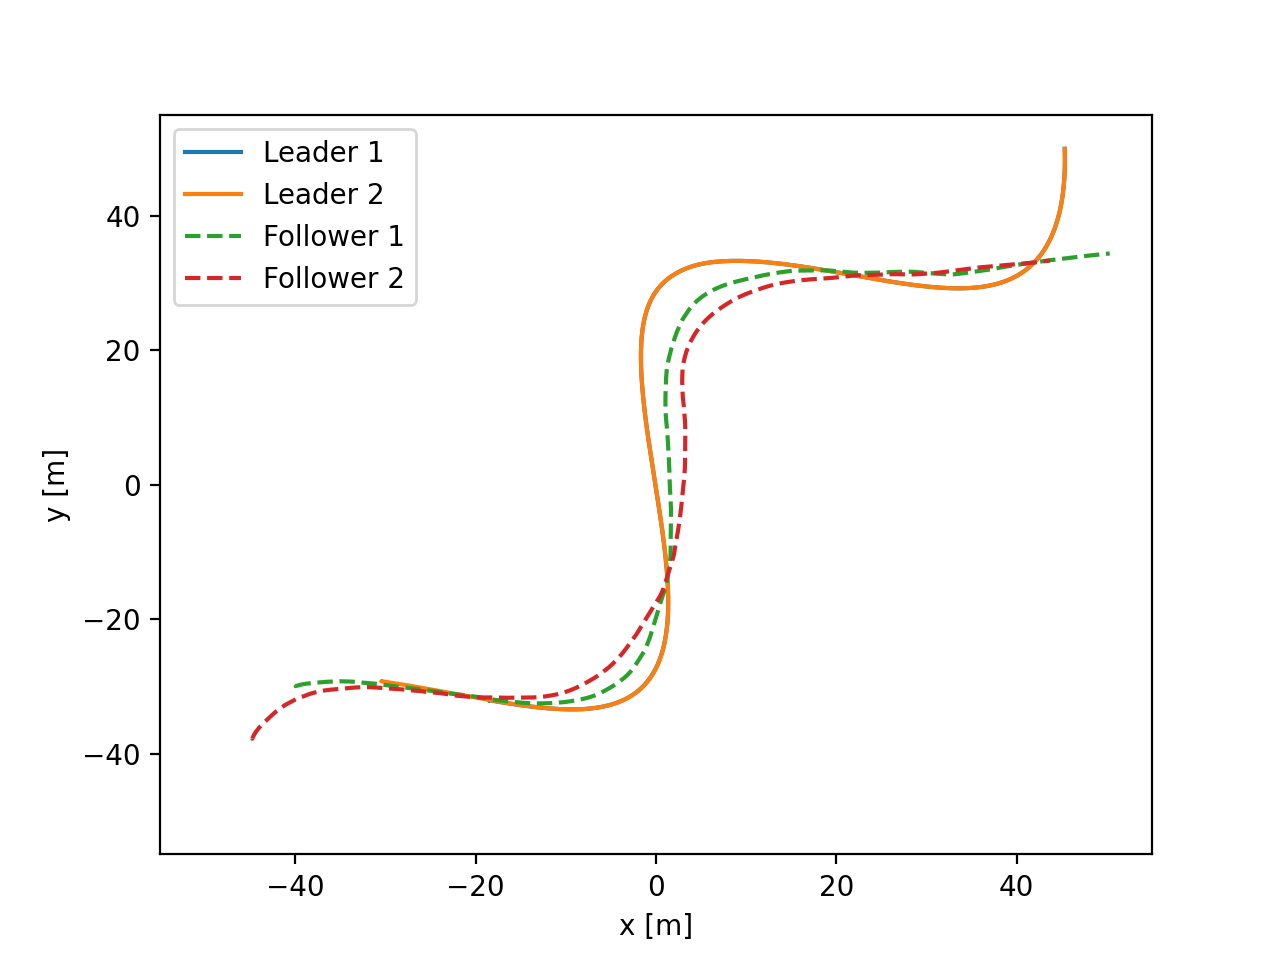
\includegraphics[height=1.8in]{Figs/Demonstration/2f_2i_soft_positions.png}}&
        \parbox[c]{2.02in}{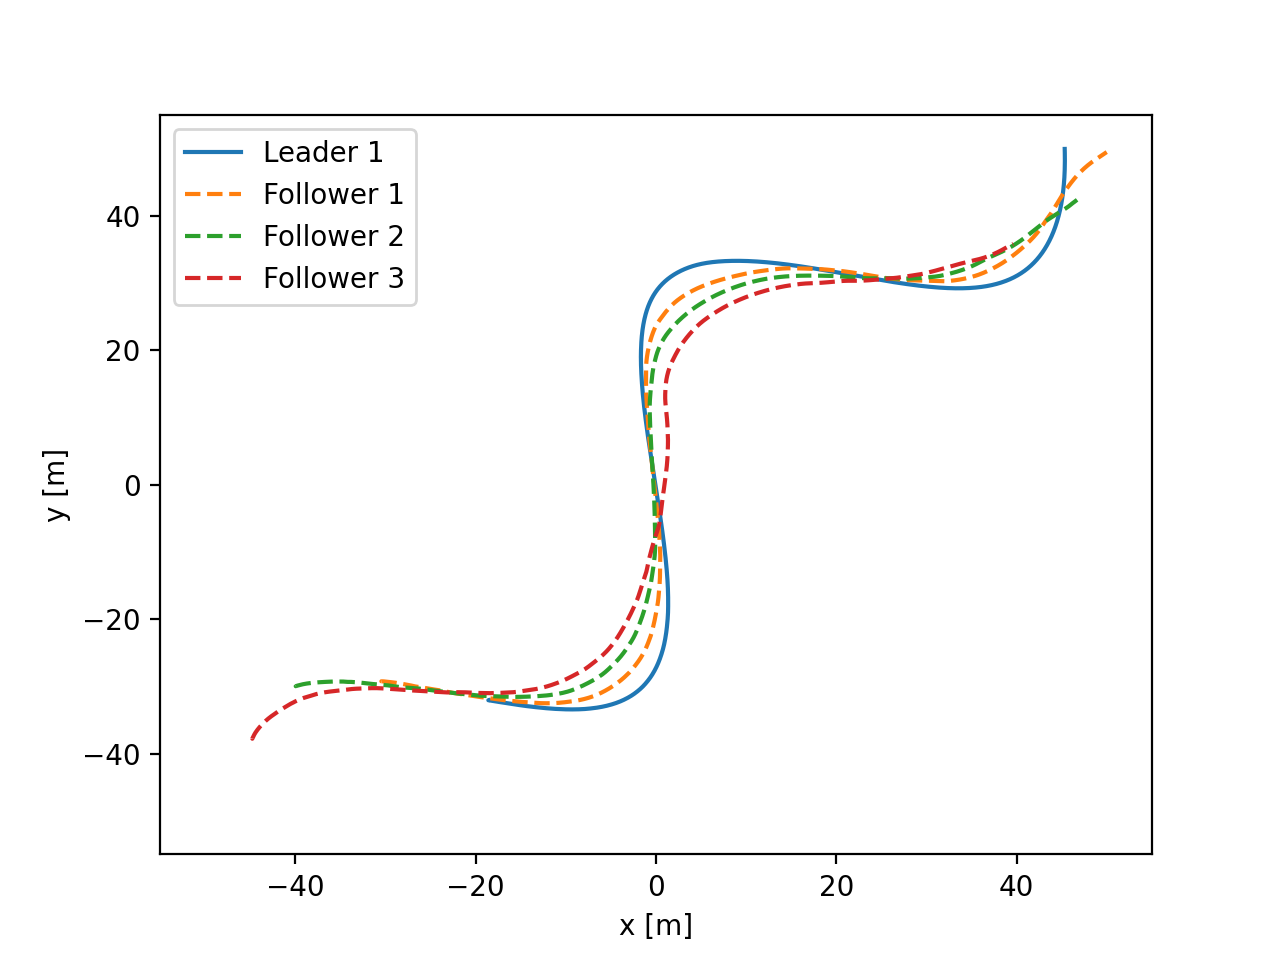
\includegraphics[height=1.8in]{Figs/Demonstration/1f_3i_soft_positions.png}}
        %\newline \\ 
        %\hline \\
    \end{tabular}
\end{table*}

In an effort to quantify the performance and robustness of the derived platooning policy, we present next results from a statistical analysis using ensemble convoy simulations. This study includes results from 128 independent simulations for each one of the three terrain types mentioned above. In order to allow relative comparisons among different terrain types as well as between follower positions in the convoy, all simulations used the 1L+3F convoy configuration and each one of the three sets of 128 simulation used the same set of randomly-generated trajectories. The performance metrics used in this analysis measure the path and speed deviation of a follower vehicle from that of the convoy's leader.

%%%  Path planning ----------------------------

The 128 distinct scenarios were created in a 100 m $\times$ 100 m swath of flat terrain. A script generated 30 randomly placed circular obstacles with sizes uniformly distributed between 5 m and 7 m. The obstacle positions were drawn from a uniform distribution with an additional restriction to allow overlap of no more than half their radius~\cite{MATLABBubbleBath}. Finally, to increase the complexity of the resulting paths and reduce the likelihood of a straight path, \textit{each} configuration included four additional fixed obstacles with radius of 8 m placed equidistant along the diagonal from start to end.

A path was designed to get from start to finish while avoiding the obstacles. 
The path start and end positions were fixed to the south-west and north-east corners, respectively. A sample obstacle field is shown on the left in Fig.~\ref{fig:synchronodemoexample}.
A Particle Swarm Optimization (PSO) algorithm~\cite{PSOObstacleAvoidance} was used to generate a shortest distance path connecting the start and end locations, as shown in the middle image of Fig.~\ref{fig:synchronodemoexample}. The path generation was constrained to produce trajectories that remained in the domain and did not intersect obstacles.

Each of the 128 resulting paths shown in Fig.~\ref{fig:synchronoallpaths} was then used as the prescribed trajectory for the path-follower PID-based lateral controller implemented on the leader vehicle, in conjunction with a PID-based longitudinal controller that prescribes a target speed linearly increasing in time (corresponding to a constant acceleration of 0.47 m/s$^2$).

To produce paths that are feasible for simulated HMMWV vehicles, the generation of the corresponding environment setup in SynChrono involved scaling obstacle meshes (rocks, trees, bushes) such that their bounding sphere allows 2 m of separation from the generated path centerline; in other words, in each of the 128 environments, the path prescribed for the leader vehicle ensures a minimum width of 4 m. An overhead view of the resulting SynChrono simulation environment is shown on the right in Figure \ref{fig:synchronodemoexample}.

%The quantitative analysis was carried out systematically as follows: 128 unique environments were created with 34 total obstacles in each, a \textit{Particle Swarm Optimization} (PSO) based algorithm calculated a possible trajectory through the environment from designated start and end points \cite{PSOObstacleAvoidance}, and then a simulation was run for each environment. In the simulation tests, the leader vehicles utilize PID-based lateral and longitudinal controllers to follow the predetermined path with a prescribed target speed (with the latter linearly increasing in time) and the follower vehicles utilize the trained network described previously.

%To produce paths feasible for a simulated HMMWV vehicle to follow, careful consideration was taken when generating each environment, its obstacles and the corresponding path through it. First, obstacles with radii of 5m to 7m were uniformly distributed across a 92 by 92 block of terrain centered at [0,0]. A check was made to ensure the obstacles only overlapped at a magnitude less than or equal to their radius \cite{MATLABBubbleBath}. Four obstacles with radii of 8m were also placed equidistant along the diagonal from start to end. This was done to increase the difficulty of the computed paths, eliminating the likelihood of straighter paths. Figure \ref{fig:obstaclegeneration} shows an example result from this obstacle generation. The positions and radii of the generated obstacles were then fed into the PSO algorithm which calculated a possible trajectory through the environment. During the computation of the candidate path, a cubic spline interpolant was calculated to verify certain conditions weren't being violated: the path didn't lead through any obstacles and that it stayed within the 92 by 92 block of terrain. The candidate path generated is shown in Figure \ref{fig:psopathgeneration}. This progression was then performed 128 times, where the obstacle positions and the candidate path represented as a bezier curve were stored to be read by \synchrono{} later. Figure \ref{fig:synchronoallpaths} shows all 128 computed paths and demonstrates the overall spread of which the candidate paths span the terrain.

%Once all 128 environments with obstacles and paths were generated, the policy was then tested with the 1L+3F configuration on the three terrain types: rigid, hard SCM, soft SCM. As a result, 384 total simulations were performed using the Euler computing cluster at the University of Wisconsin-Madison. For each simulation, the corresponding environmental factors were loaded in: obstacles and path to follow. As seen in Figure \ref{fig:psopathgeneration}, the generated path is extended close to the edge of some obstacles. When loaded into \chrono{}, the obstacle meshes were scaled so that their new radii allowed for 2m of separation from the prescribed path to the mesh. This was done to provided adequate space for the leader to drive through the environment without hitting an obstacle asset. An overhead view of the resulting simulation environment in \synchrono{} is shown in Figure \ref{fig:synchronodemoexample}.

% \begin{figure}
%     \centering
%     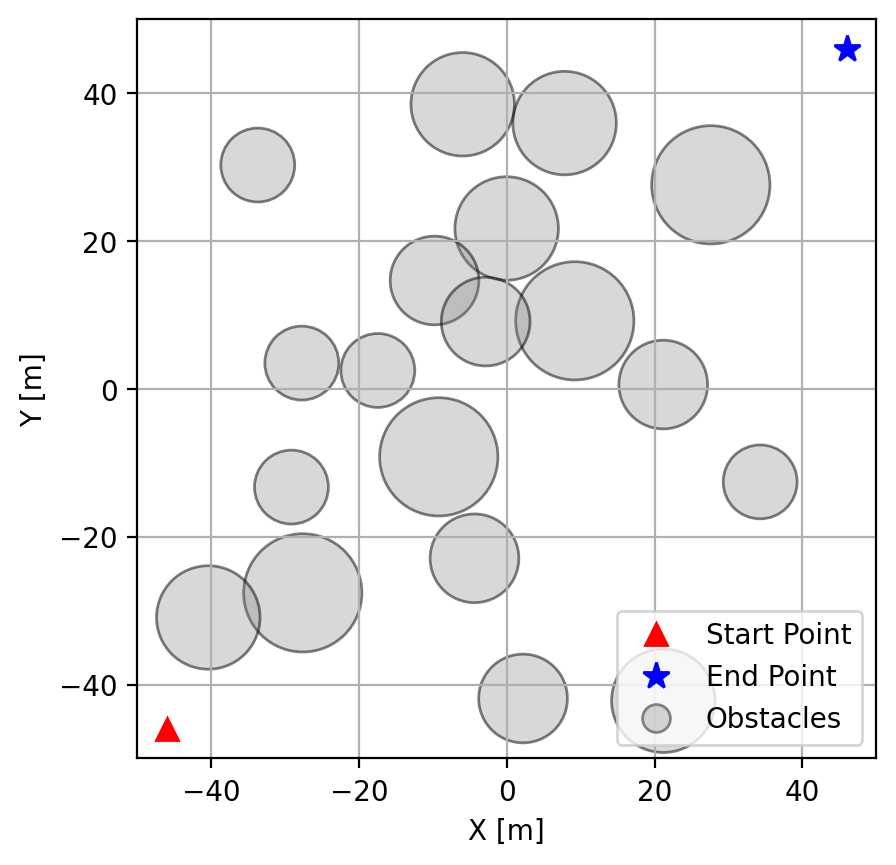
\includegraphics[width=\columnwidth]{Figs/StatisticalAnalysis/obst_gen_68.png}
%     \caption{Sample obstacle field.}   
%     \label{fig:obstaclegeneration}
% \end{figure}

% \begin{figure}
%     \centering
%     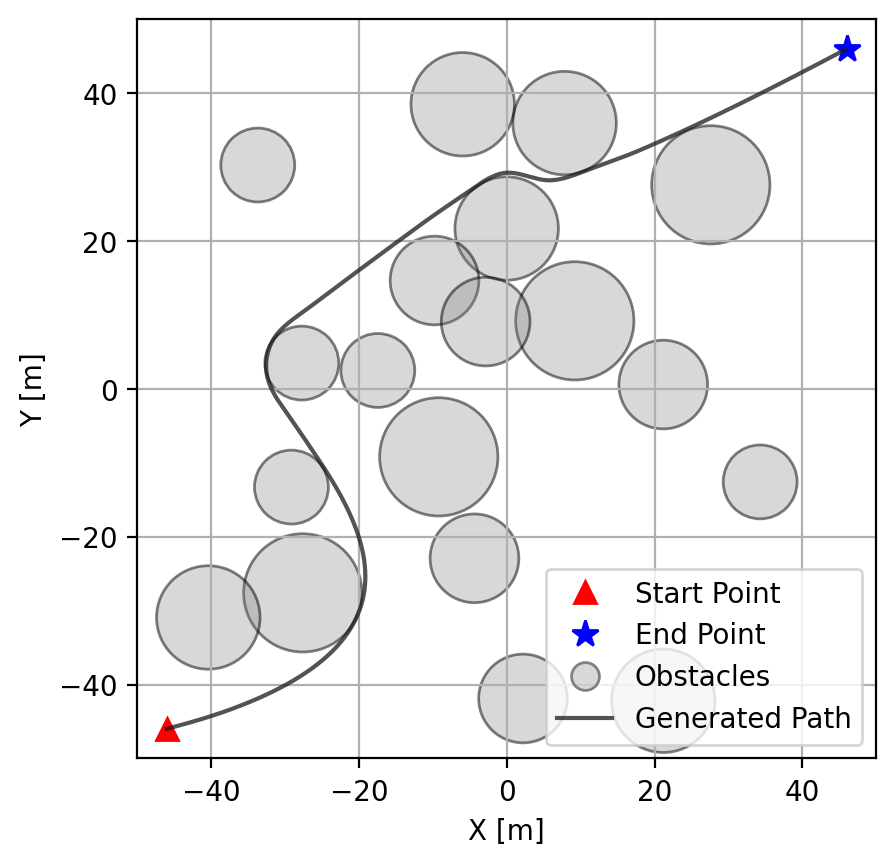
\includegraphics[width=\columnwidth]{Figs/StatisticalAnalysis/path_gen_68.png}
%     \caption{Sample PSO-based path planning.}   
%     \label{fig:psopathgeneration}
% \end{figure}

% \begin{figure}
%     \centering
%     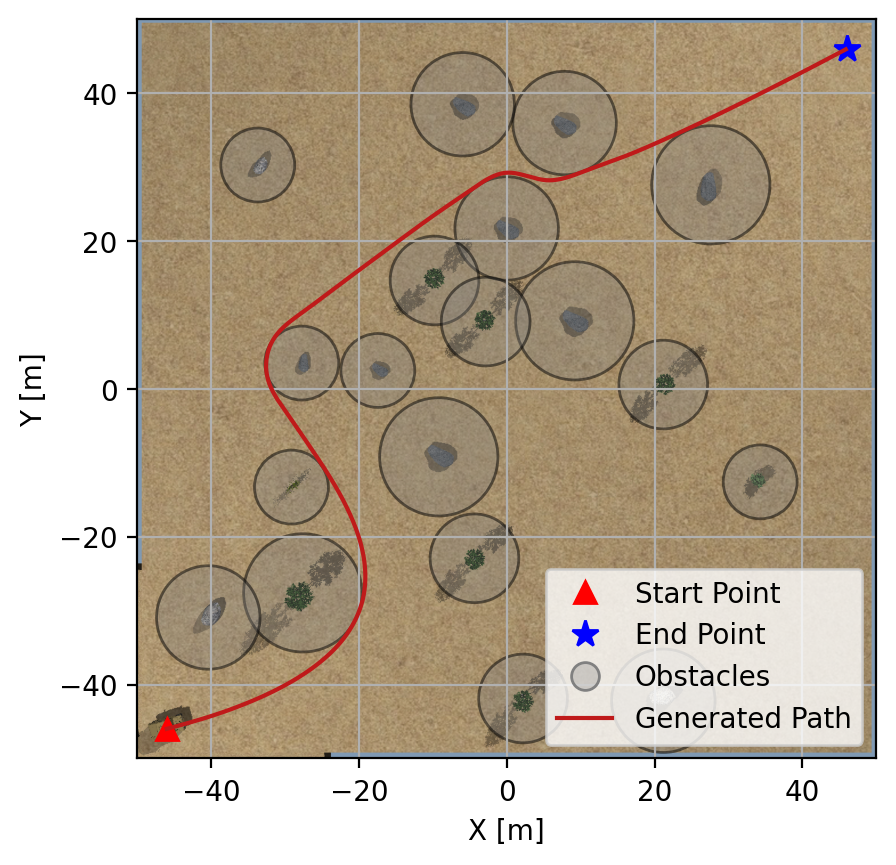
\includegraphics[width=\columnwidth]{Figs/StatisticalAnalysis/path_gen_rigid_68.png}
%     \caption{Overhead view of the corresponding SynChrono environment setup.}   
%     \label{fig:synchronodemoexample}
% \end{figure}

\begin{figure*}
    \centering
    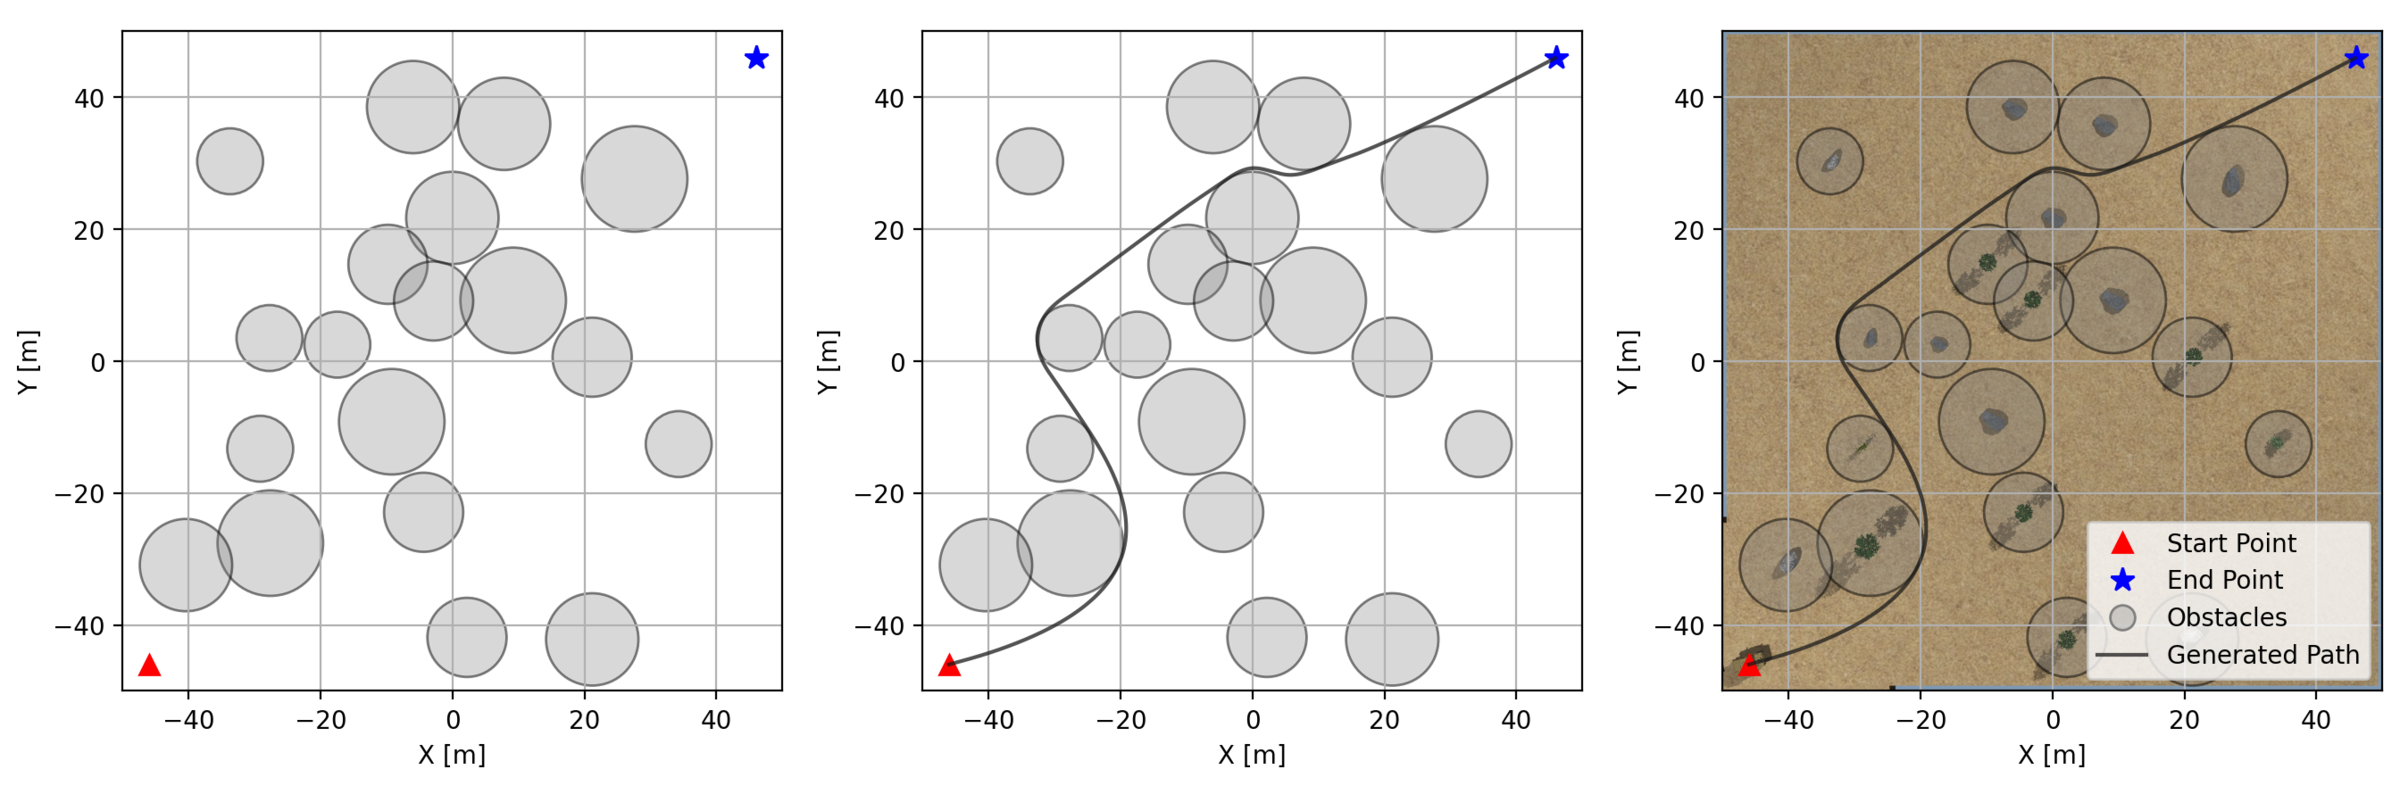
\includegraphics[width=\textwidth]{Figs/StatisticalAnalysis/path_gen_progression.png}
    \caption{Sample obstacle field, PSO-based path planning, and the corresponding SynChrono environment setup.}   
    \label{fig:synchronodemoexample}
\end{figure*}

\begin{figure}
    \centering
    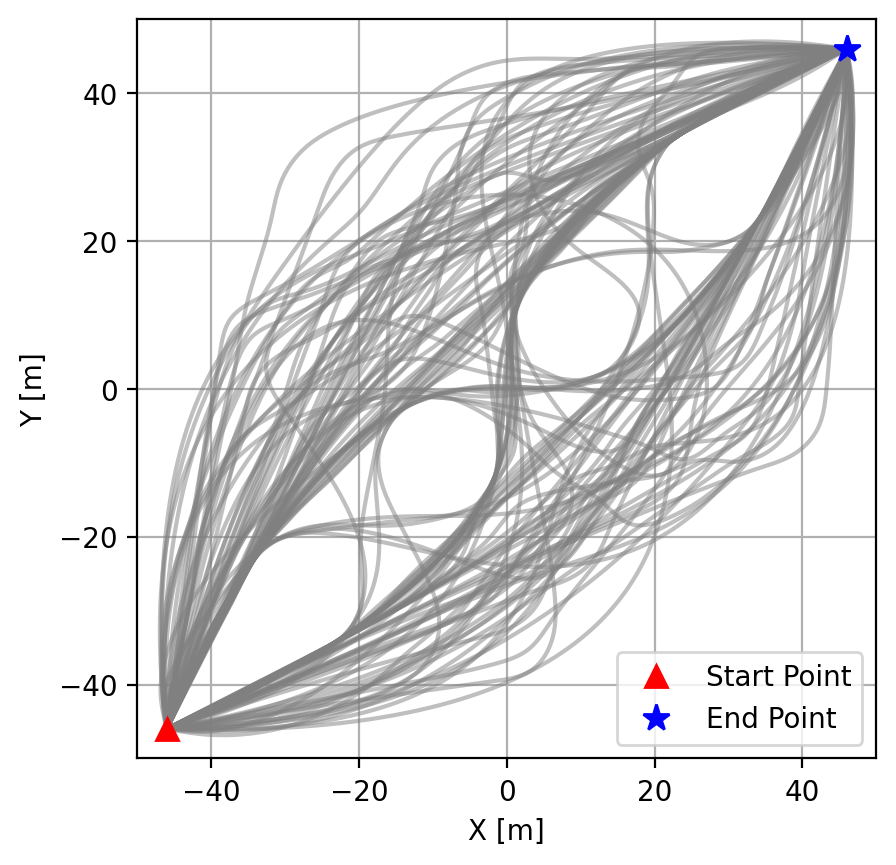
\includegraphics[width=\columnwidth]{Figs/StatisticalAnalysis/all_possible_paths.png}
    \caption{Ensemble of the 128 paths used in the statistical analysis.}   
    \label{fig:synchronoallpaths}
\end{figure}

%%%  Metrics ----------------------------

In order to perform a statistical analysis of the performance of the platooning policy, we define a set of six performance metrics that measure the deviations of a follower vehicle from that of the convoy leader and encode both lateral path deviation and deviations in the vehicle speed at a given location along the leader's path.  These metrics are defined in such a way as to allow comparisons between the performance of followers at different positions in the convoy, as well as across the three different terrain types considered here.

To eliminate differences due to the fact that vehicles in a convoy are inherently staggered along the path, the evaluation of the performance metrics is based on a common path segment.  Figure~\ref{fig:metrics_path} illustrates this process for the same trajectory used as an example before. The sample results used in this description are results of a simulation on rigid terrain and consider the last vehicle in the convoy (Follower 3).  The start clip point is defined as the point on the follower path closest to the leader's initial location. Similarly, the end clip point is defined as the point on the leader's path closest to the follower's final location.  The resulting segment on the leader's path is then sampled at intervals of equal arc-length and the closest point on the follower's path to each such sampled point is identified. The distance between corresponding points on the leader and follower paths are then used to define a {\em follower path deviation} as function of distance traveled along the leader's path (see Fig.~\ref{fig:metrics_path_deviation}).  This allows us to define the first two performance metrics: $m_{p}^{avg}$, the average follower path deviation, and $m_{p}^{max}$, the maximum path deviation.

Next, we compare the vehicle speeds at corresponding points on the follower and leader paths as shown in the left plot of Fig.~\ref{fig:metrics_speed_deviation} from which we derive the absolute and relative speed errors (the latter being the speed difference scaled by the leader's speed at that location).  The underlying assumption in these definitions is that a follower's speed should match as closely as possible the speed of the leader vehicle at the same location on the path (and not at the same point in time); this is also why, when calculating the subsequent speed deviation metrics, we discard the values corresponding to the first 10 m of travel (to allow the vehicles to accelerate from rest to the desired convoy speed).  With these we define two more pairs of performance metrics: $m_{as}^{avg}$, $m_{as}^{max}$, for the average and maximum absolute speed deviation between leader and follower, and $m_{rs}^{avg}$, $m_{rs}^{max}$, for the average and maximum relative speed deviation of the follower.

\begin{figure}
    \centering
    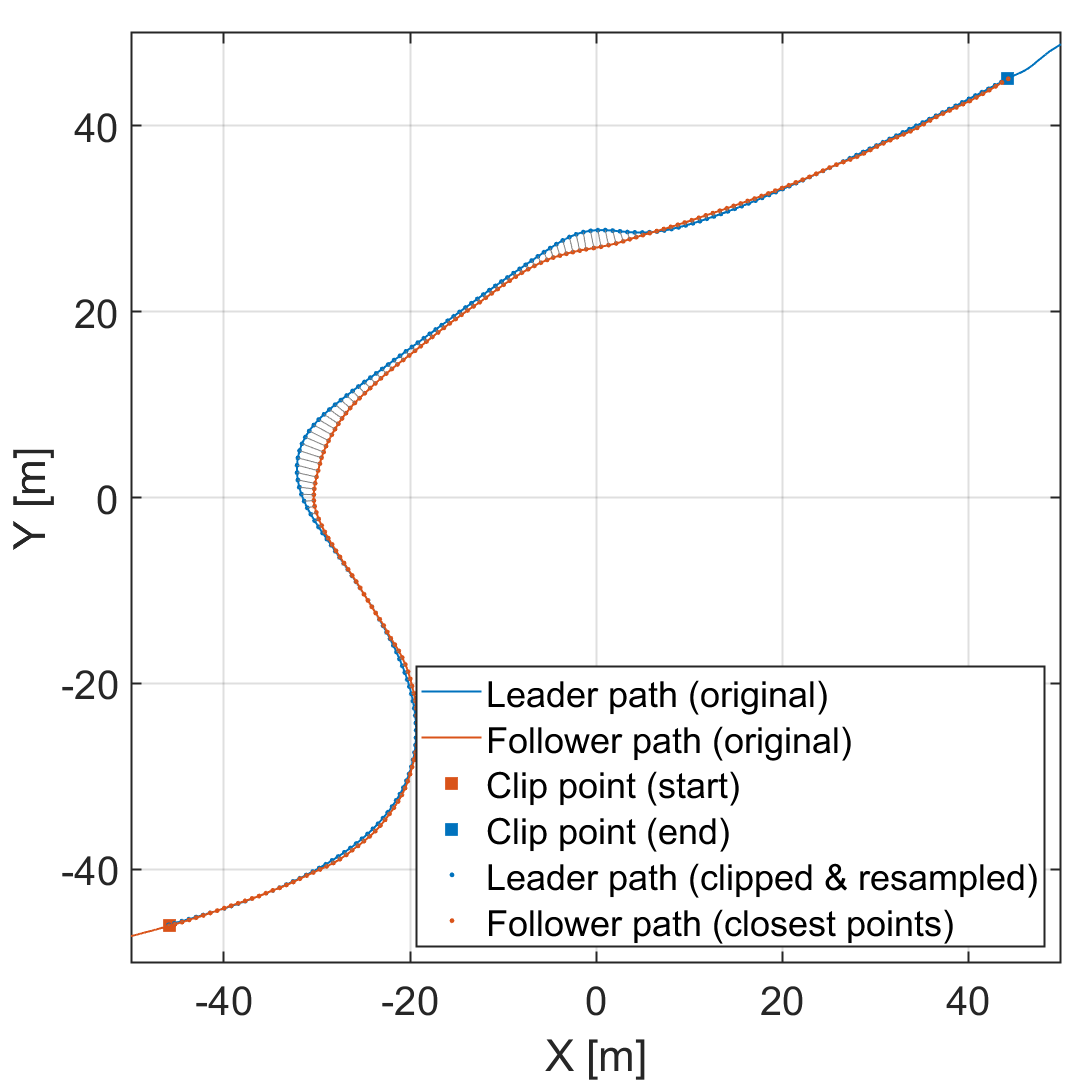
\includegraphics[width=0.9 \columnwidth]{Figs/Metrics/path.png}
    \caption{Path deviation metrics calculation (rigid terrain, Follower 3). The segment of the leader path used in calculations for this particular scenario (rigid terrain) was $L = 158.2 \text{ m}$.}
    \label{fig:metrics_path}
\end{figure}

\begin{figure}
    \centering
    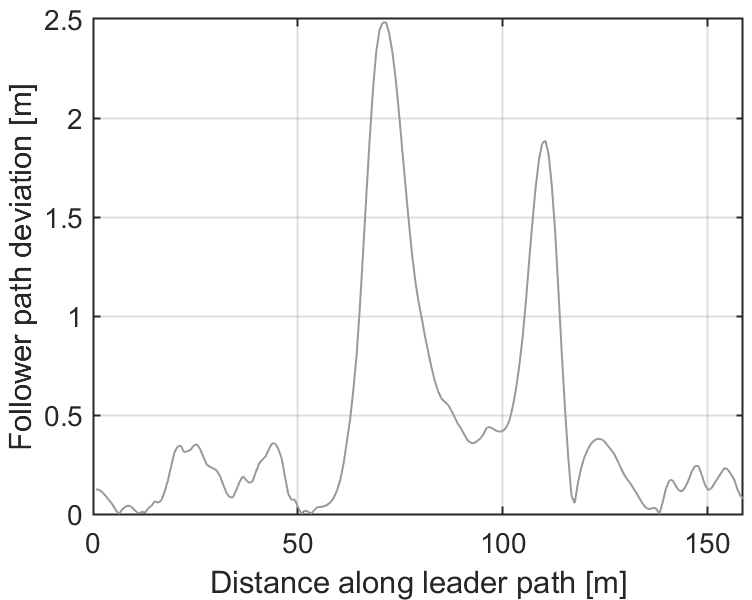
\includegraphics[width=0.9\columnwidth]{Figs/Metrics/path_deviation.png}
    \caption{Deviation in path between Leader and Follower 3. The lateral deviation metrics for this particular scenario (rigid terrain) were $m_{p}^{avg} = 0.473 \text{ m}$, $m_{p}^{max} = 2.484 \text{ m}$.}   
    \label{fig:metrics_path_deviation}
\end{figure}

\begin{figure*}
    \centering
    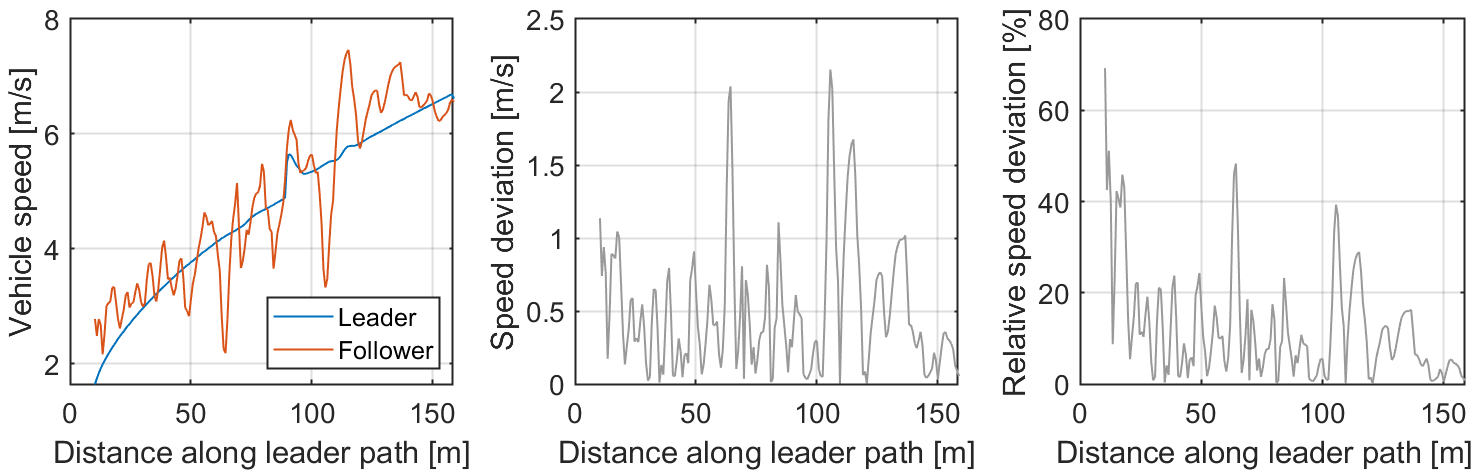
\includegraphics[width=0.9\textwidth]{Figs/Metrics/speed_deviation.png}
    \caption{Deviation in speed between Leader and Follower 3.  The vehicle speeds are evaluated at the same location along the leader's path. The speed deviation metrics for this particular scenario (rigid terrain) where $m_{as}^{avg} = 0.505 \text{ m/s}$, $m_{as}^{max} = 2.154 \text { m/s}$ and $m_{rs}^{avg} = 12.2 \%$, $m_{rs}^{max} = 69.2 \%$.}   
    \label{fig:metrics_speed_deviation}
\end{figure*}


%%%  Statistical analysis ----------------------------

The six metrics defined above were evaluated for each of the three follower vehicles in each scenario in the three sets of 128 environments on rigid, SCM-Hard, and SCM-Soft terrain, respectively. The resulting statistics are presented as box-and-whisker diagrams in Figs.~\ref{fig:metricpath}, \ref{fig:metricspeed}, and \ref{fig:metricrelspeed}, providing measures of the variability in the three statistical populations without any assumption on their underlying statistical distribution (which is unknown, due to the manner in which the sample trajectories were constructed).  For each metric, on each terrain type and for each of the three follower vehicles in the 1L+3F configuration, these standard box plots provide information on their mean, second and third quartiles, as well as minimum and maximum values.

We assume that a perfect control policy for a follower vehicle would result in a convoy in which each follower vehicle runs exactly in the tracks of the vehicle preceding it and achieves the exact same speed at any given location.  Given their definition, this ideal case corresponds to zero values for each of the six performance metrics.  

The results of the statistical analysis presented herein confirm the intuition that, in a 1L+3F configuration, a less than perfect control policy will lead to worse performance for the trailing follower vehicles and better performance on harder surfaces (especially taking into account that the training was performed exclusively on rigid terrain).  However, as the results for both path and speed deviation show, this is not the case when comparing performance on SCM-Hard and SCM-Soft terrains, with the latter showing consistent lower metrics values (i.e., better performance in terms of maintaining position in the convoy). 

The explanation for this behavior is likely a combination of several factors.  First, even though the target speed profile for the leader vehicle was set identically for all three terrain types, the increased terrain resistance in the SCM-Hard and SCM-Soft cases resulted in the leader vehicle being unable to continuously increase its speed to the specified value; on both deformable terrain types, the vehicles were unable to shift in the higher gears and their speed limited to lower levels than on rigid terrain (an effect more pronounced on SCM-Soft terrain than on SCM-Hard). The ensuing overall lower convoy speed results in driving scenarios where the control policy can adapt better.  
%
Second, as seen in Fig.~\ref{fig:metrics_speed_deviation} and typical of all simulations conducted as part of this analysis, current deficiencies in the RL-based control policy result in relatively jerky motion of the follower vehicles and noisy speed profiles.  These spurious accelerations and decelerations are inhibited on the SCM-Soft due to the increased motion resistance.
%
Finally, the largest deviations in a follower's path (see Fig.~\ref{fig:metrics_path}) always occur at tight turns where the leader vehicle must go around an obstacle.  In these situations, the tendency of the control policy is to ``cut corners'' and thus direct the vehicle to increase steering input.  However, these control steering inputs are more difficult to follow in a deformable terrain soft enough to result in deep ruts, thus resulting in the follower vehicles more closely matching the leader's vehicle path around obstacles.


While the path planning procedure and the path-following PID-based control policy implemented for the leader vehicles ensures that a leader vehicle always avoids obstacles, this is not the case for the RL-based control policy implemented for the follower vehicles, which occasionally are unable to avoid an obstacle (in few situations, a follower vehicle, especially one in position 2 or 3, may end up going on the opposite side of an obstacle).  This behavior has multiple compounding causes, including the particular reward system used in the current training as well as configurations where perception of the leader vehicle is obstructed by an obstacle or the leader vehicle is out of the camera sensor's field of view while negotiating a tighter turn.
%
The paths of all vehicles on each terrain type are shown in Fig.~\ref{fig:pathsranksall}. The path information therein is used to gauge the robustness of the control policy in terms of obstacle avoidance. Figure~\ref{fig:obstacleshit} provides the cumulative statistics in terms of number of obstacles hit, over all ensemble simulations, for all three terrain types and for each of the three follower vehicles.  These results show the same relative performance trends observed before, with the trailing follower on SCM-Hard terrain exhibiting worst performance. 


%Using the data collected during each of the 384 simulations, the aforementioned metric calculations were performed and their results recorded for subsequent analysis, of which is presented here.

%To gauge the overall performance of the policy, where the primary goal is that the follower drives in the tracks of its leader, the integrated error metric is most insightful. A better control policy would produce a smaller integrated error metric and when Figure \ref{fig:metricpathavg} is examined, it can be seen the SCM hard simulations produces disproportionally larger values. The comparative performance between rigid and SCM soft isn't as evident; however, the tests performed on rigid do behave better than SCM soft for the followers at depths 1 and 2, but approximately the same for follower 3. Furthermore, the spread for rigid is far less than that for SCM hard and SCM soft for follower 1 and 2. For follower 3, the spread between the rigid and SCM soft experiments is approximately equal, where as the SCM hard is quite larger. A possible explanation for the performance drop experienced by the tests on SCM hard could be attributed to the friction associated with a deformable terrain (i.e. there is more friction at the wheels, so the policy has difficulty reacting to this new stimuli). This hypothesis is contradicted by the SCM soft tests; however, a suitable explanation could be the fact the SCM soft is \textit{considerably} softer than the harder parameters and produces very deep ruts; hard enough, in fact, that it could mean the vehicle has more difficulty escaping the ruts of it's leader. These ideas are also evident in Figure \ref{fig:pathsranksall} and Figure \ref{fig:obstacleshit}, where they show the path taken and the number of obstacles hit by each vehicle, respectively.

%Similar to the integrated path error, the maximum deviation is also insightful when attempting to analyze how the policy performs. Most prominent for paths where tight corners are present, significant deviations from the leaders path could result in the follower clipping obstacles or failing to see its leader all together. As shown in Figure \ref{fig:metricpathmax}, rigid is consistently better than both the SCM experiments. One simple explanation for this discrepancy is the fact that vehicles drive faster on the rigid terrain, meaning the foresight to make a turn must be greater and vehicle ends up cutting corners less. In addition, the policy was trained on rigid terrain, which could represent a fault of this approach. Moreover, the SCM soft tests typically have maximum deviations less than that of the SCM hard tests. This can be explained again by the fact that the snow-like soft SCM parameters result in the vehicle staying in the tracks of its leader more often.

%As alluded to before, the speed of the SCM tests are far less than that for the rigid terrain trials. The friction associated with the deformable terrain is too great for the vehicle to reach its shift points. This results in decreased overall speeds for the vehicles simulated on soft and hard SCM. The soft SCM is also much softer than the hard SCM terrain, so its speed is also frequently smaller. This would mean that the integrated error between the speed of the follower and the leader would be less because of the lower speeds, seen in Figure \ref{fig:metricspeedavg}. This trend is also present in the maximum velocity deviation from the leader, shown in Figure \ref{fig:metricspeedmax}. Due to the simple fact that the SCM simulations run at lower speeds, the maximum speed deviation will be less.

% \begin{figure}
%     \centering
%     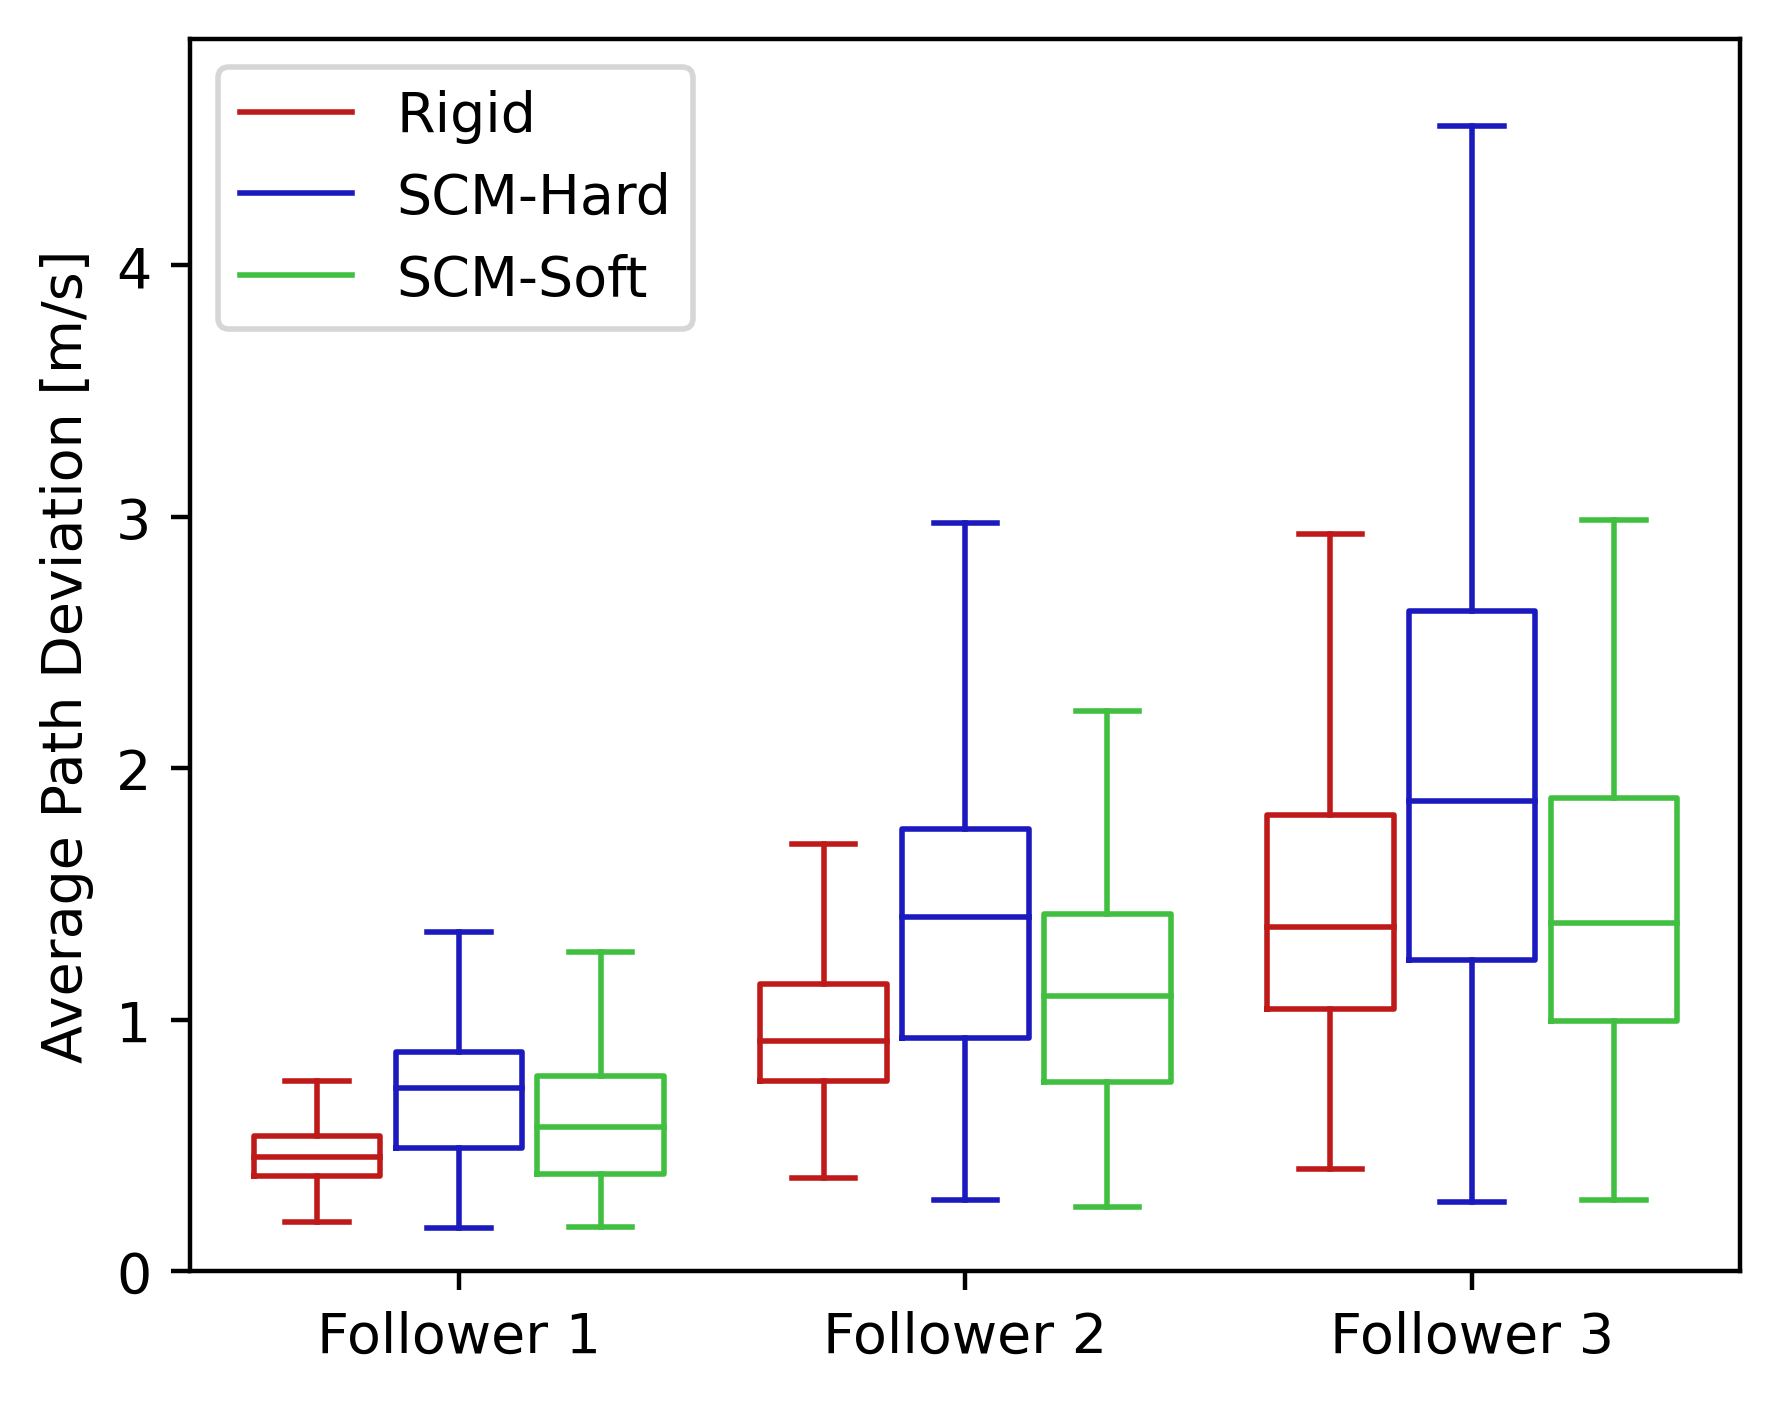
\includegraphics[width=\columnwidth]{Figs/StatisticalAnalysis/metric_path_avg.png}
%     \caption{Integrated error of the position between the followers and leaders path's.}   
%     \label{fig:metricpathavg}
% \end{figure}

% \begin{figure}
%     \centering
%     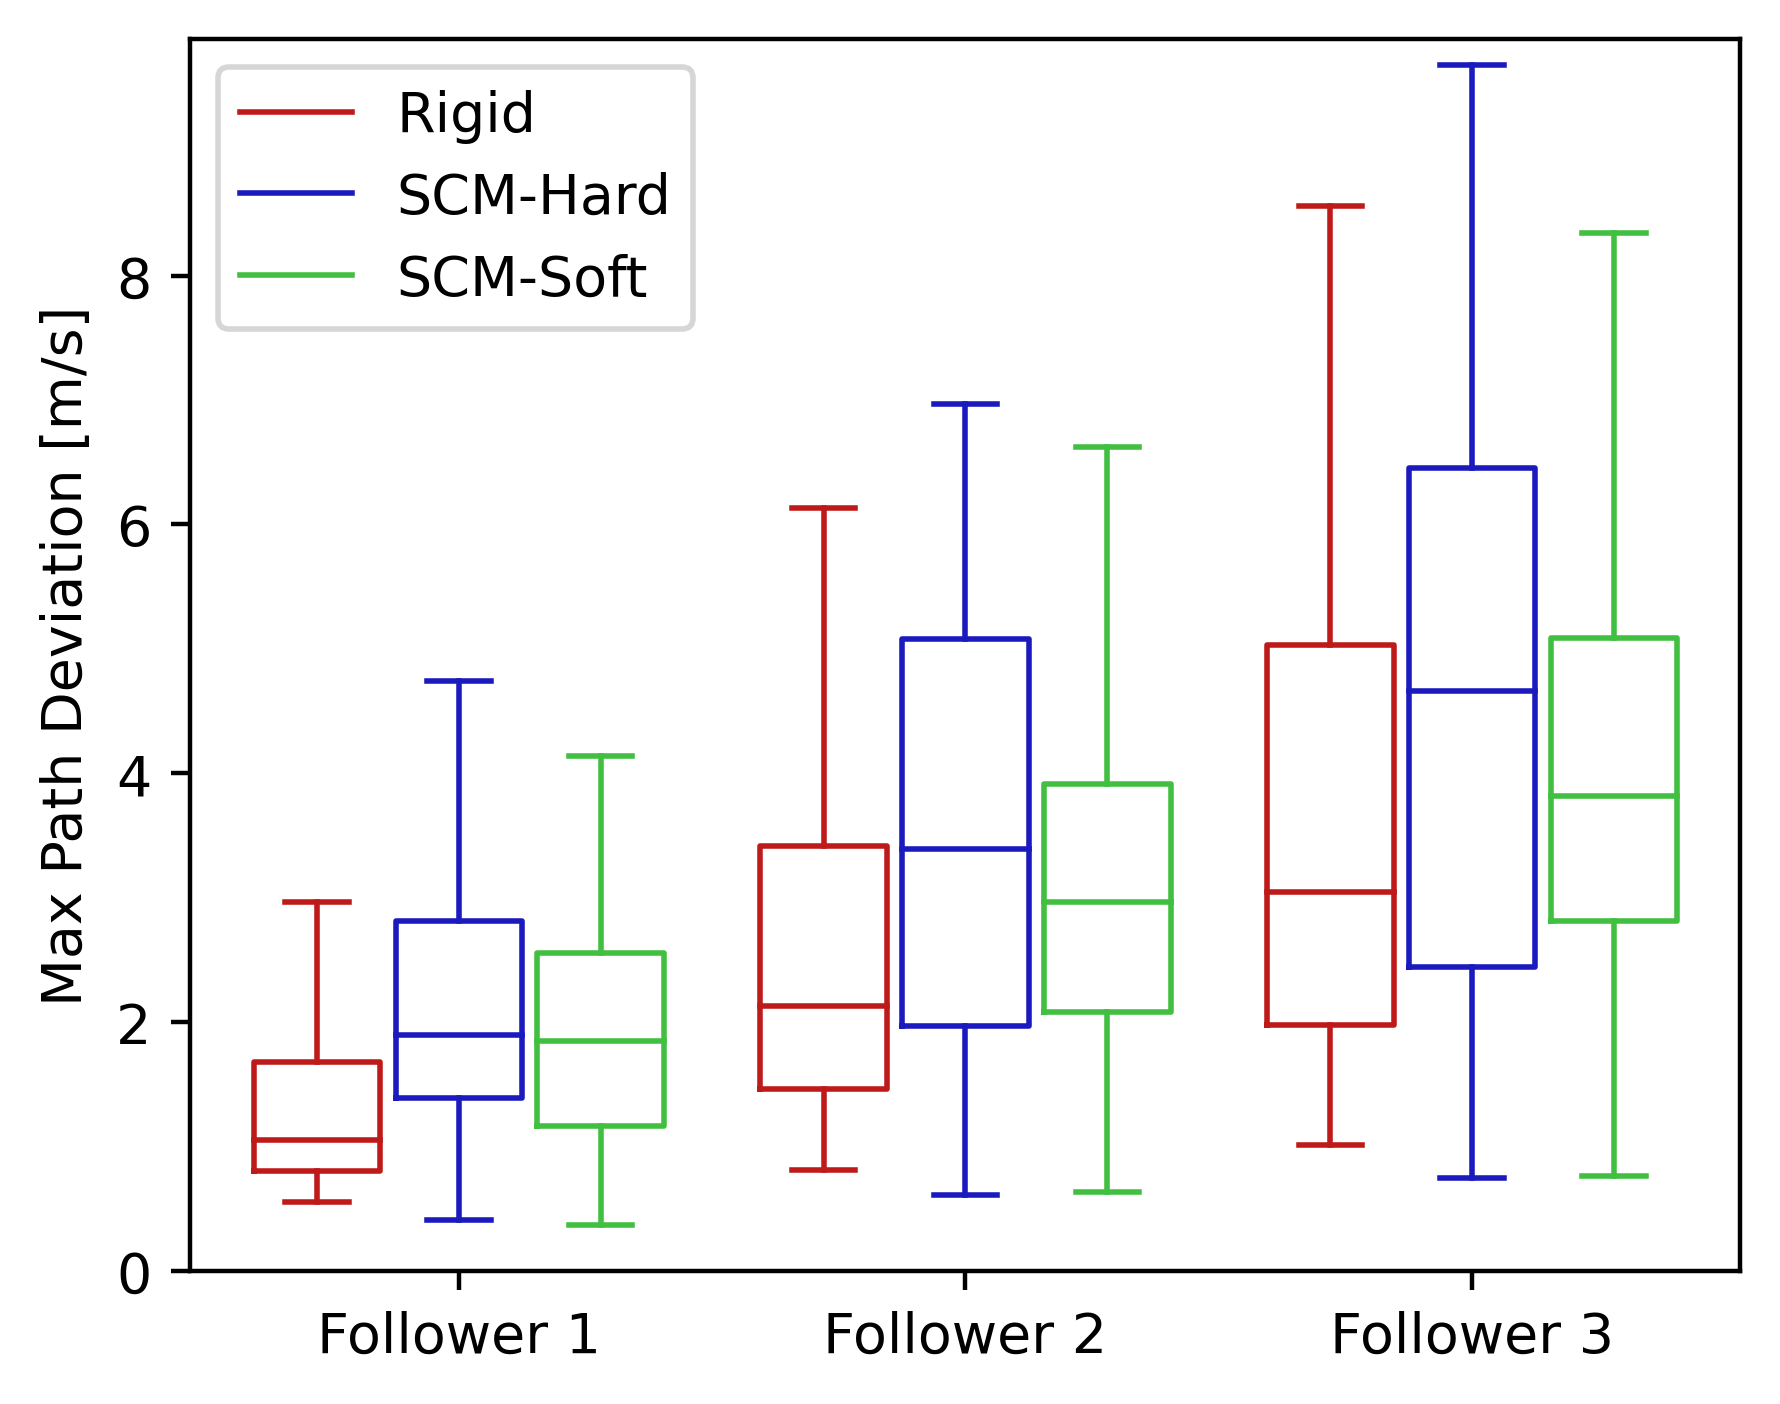
\includegraphics[width=\columnwidth]{Figs/StatisticalAnalysis/metric_path_max.png}
%     \caption{Maximum deviation metric between the followers and leaders path's.}   
%     \label{fig:metricpathmax}
% \end{figure}

% \begin{figure}
%     \centering
%     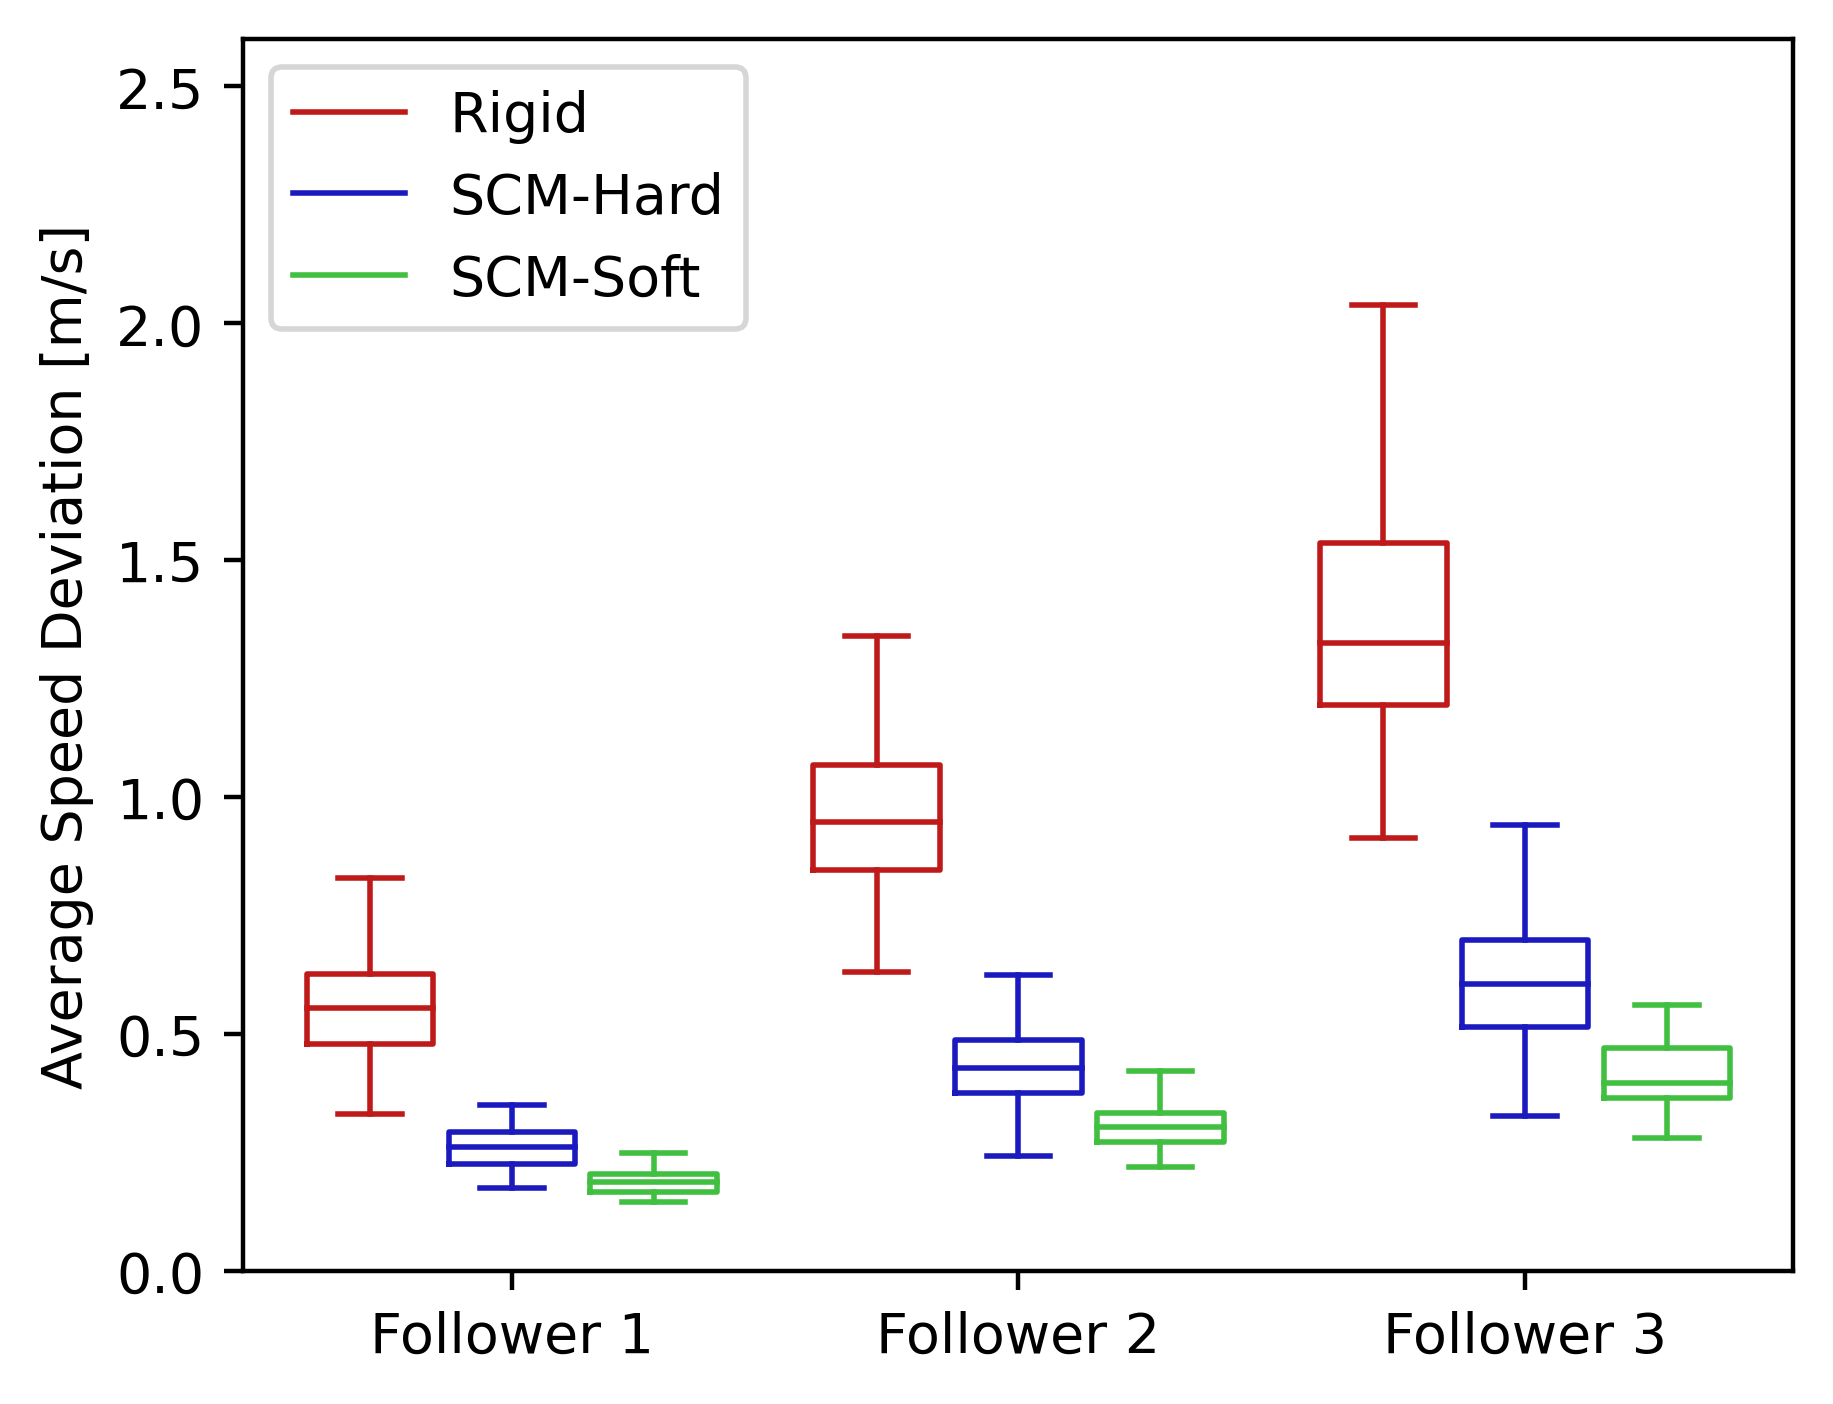
\includegraphics[width=\columnwidth]{Figs/StatisticalAnalysis/metric_speed_avg.png}
%     \caption{Integrated error between the followers and leaders velocity profile's.}   
%     \label{fig:metricspeedavg}
% \end{figure}

\begin{figure*}
    \centering
    \begin{subfigure}{0.45\textwidth}
        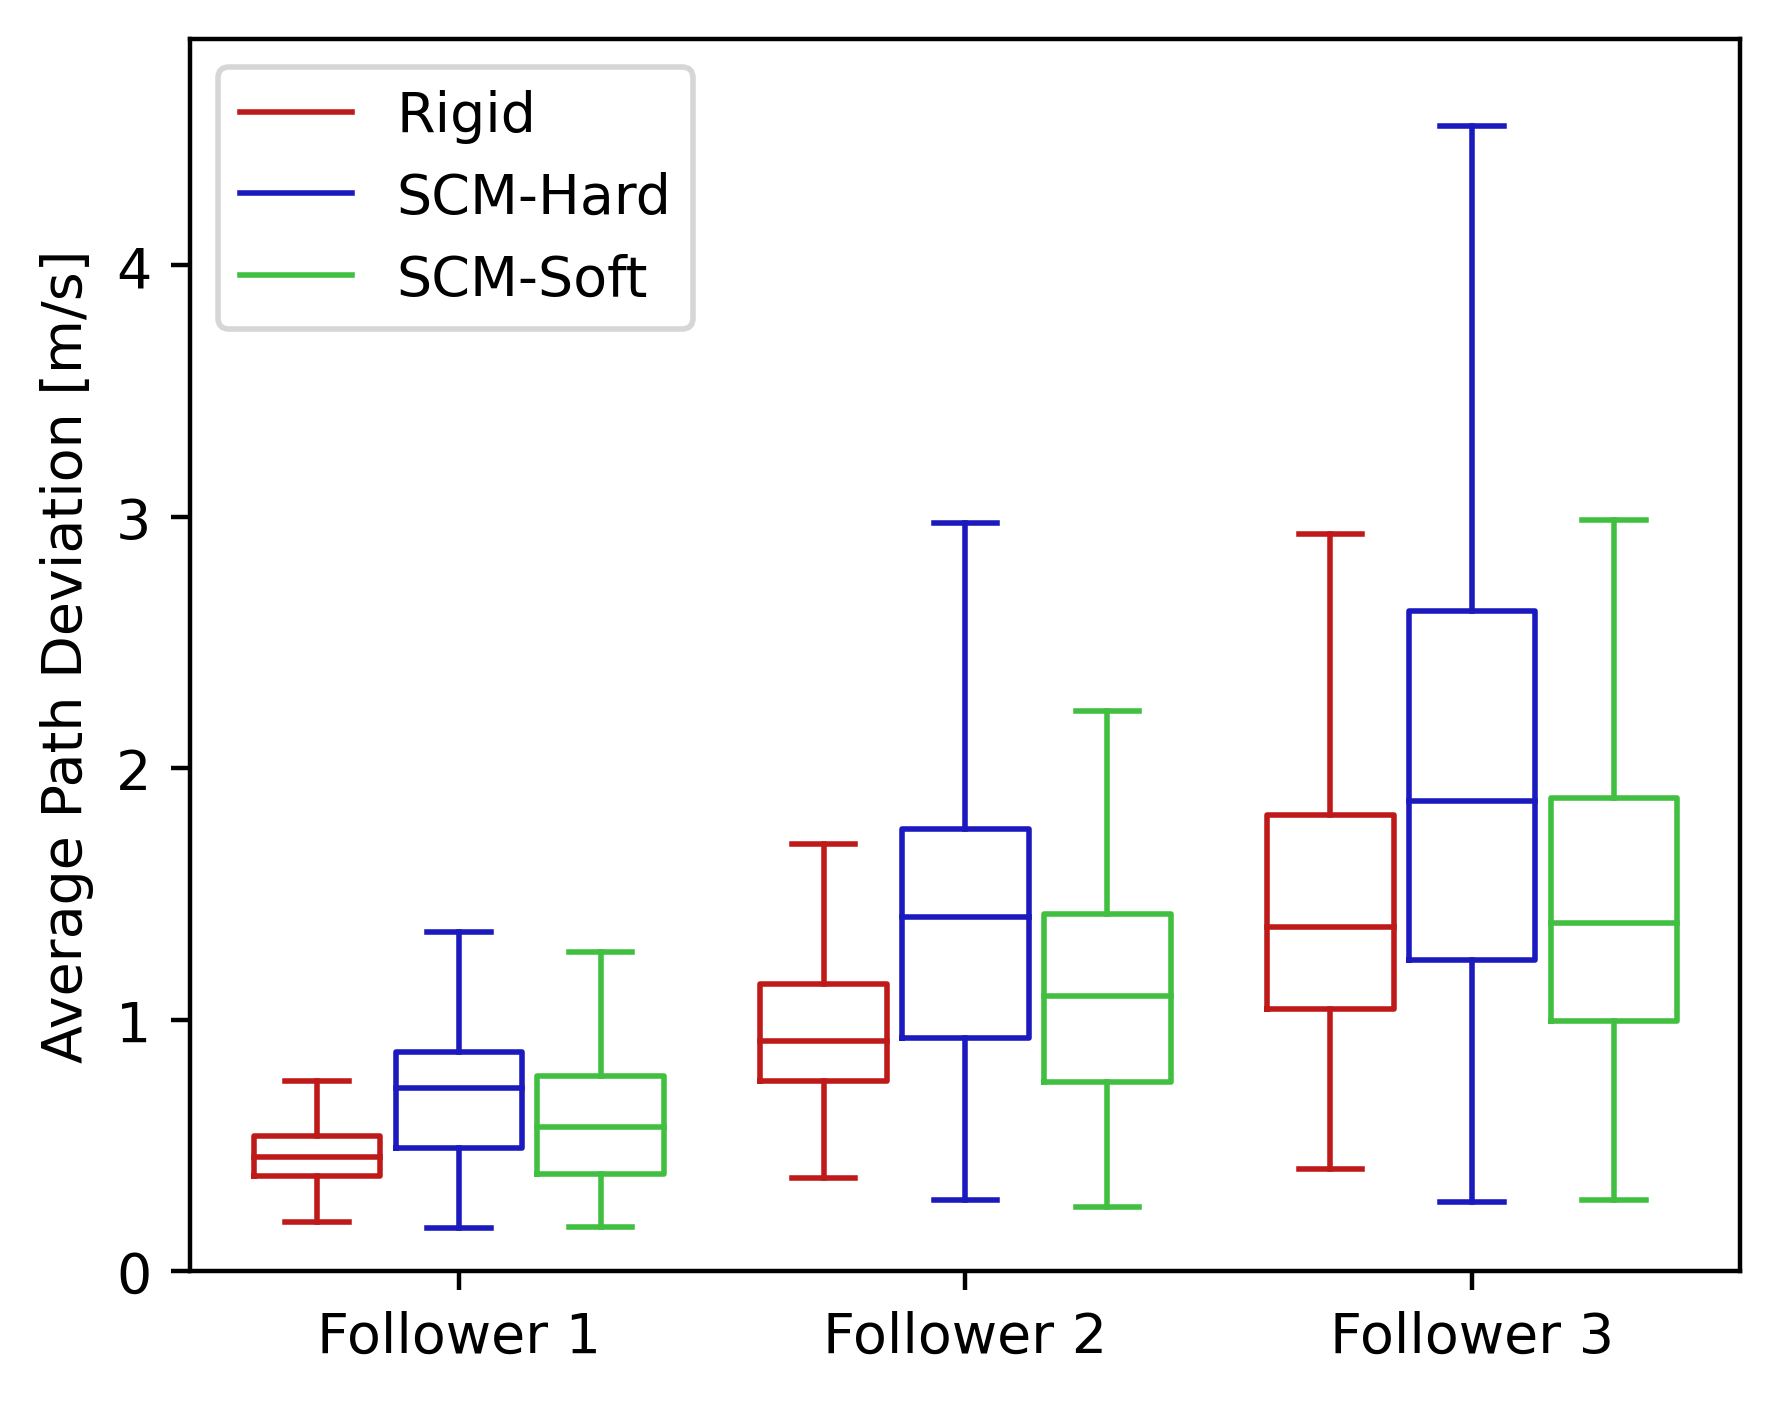
\includegraphics[width=\columnwidth]{Figs/StatisticalAnalysis/metric_path_avg.png}
        \caption{} \label{fig:metricpathavg}
    \end{subfigure}
    \begin{subfigure}{0.45\textwidth}
        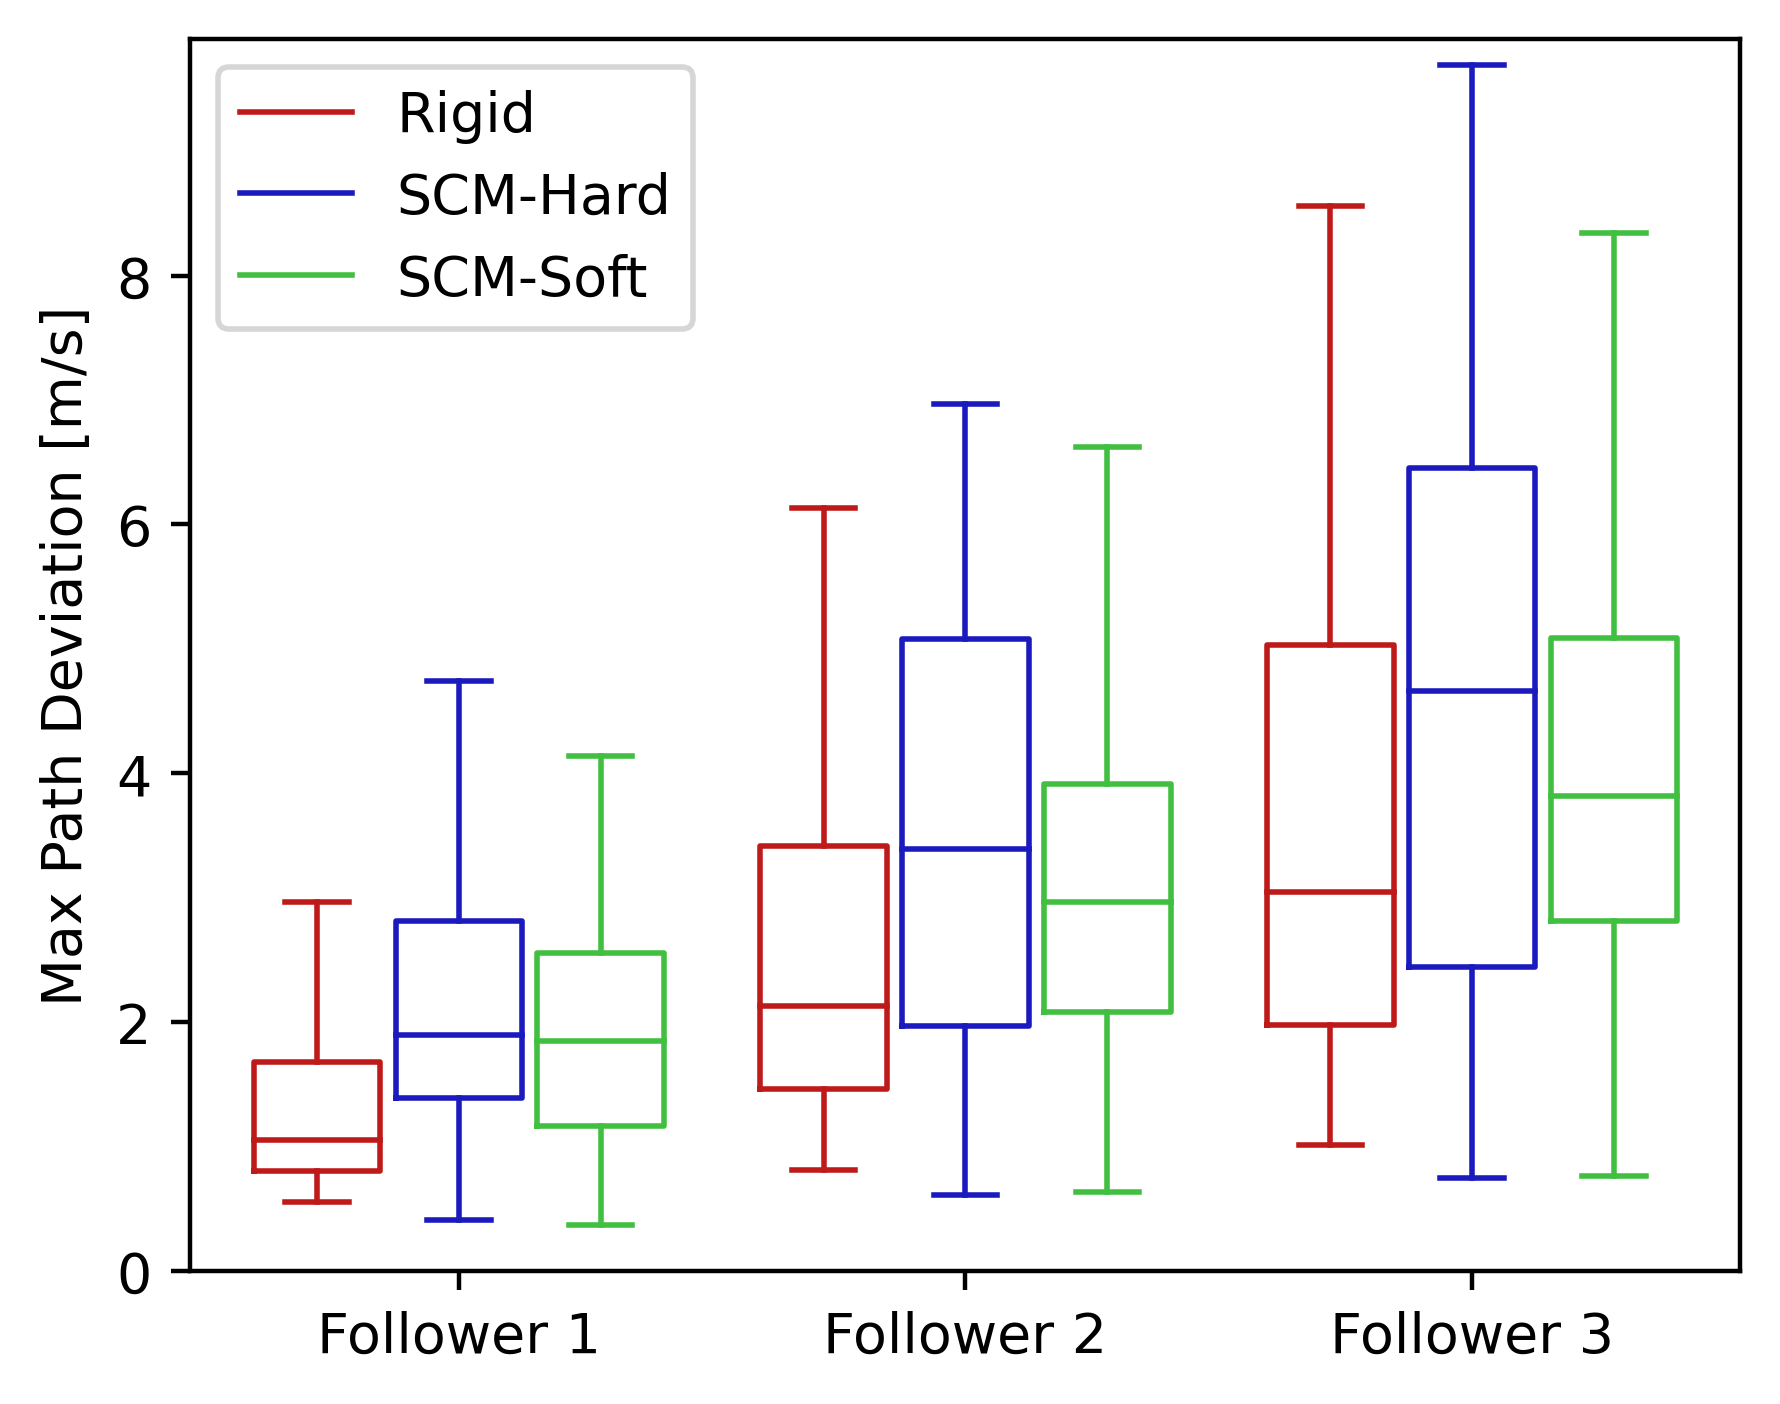
\includegraphics[width=\columnwidth]{Figs/StatisticalAnalysis/metric_path_max.png}
        \caption{} \label{fig:metricpathmax}
    \end{subfigure}%
    \caption{Statistics of average and maximum follower path deviations.}  
    \label{fig:metricpath}
\end{figure*}

\begin{figure*}
    \centering
    \begin{subfigure}{0.45\textwidth}
        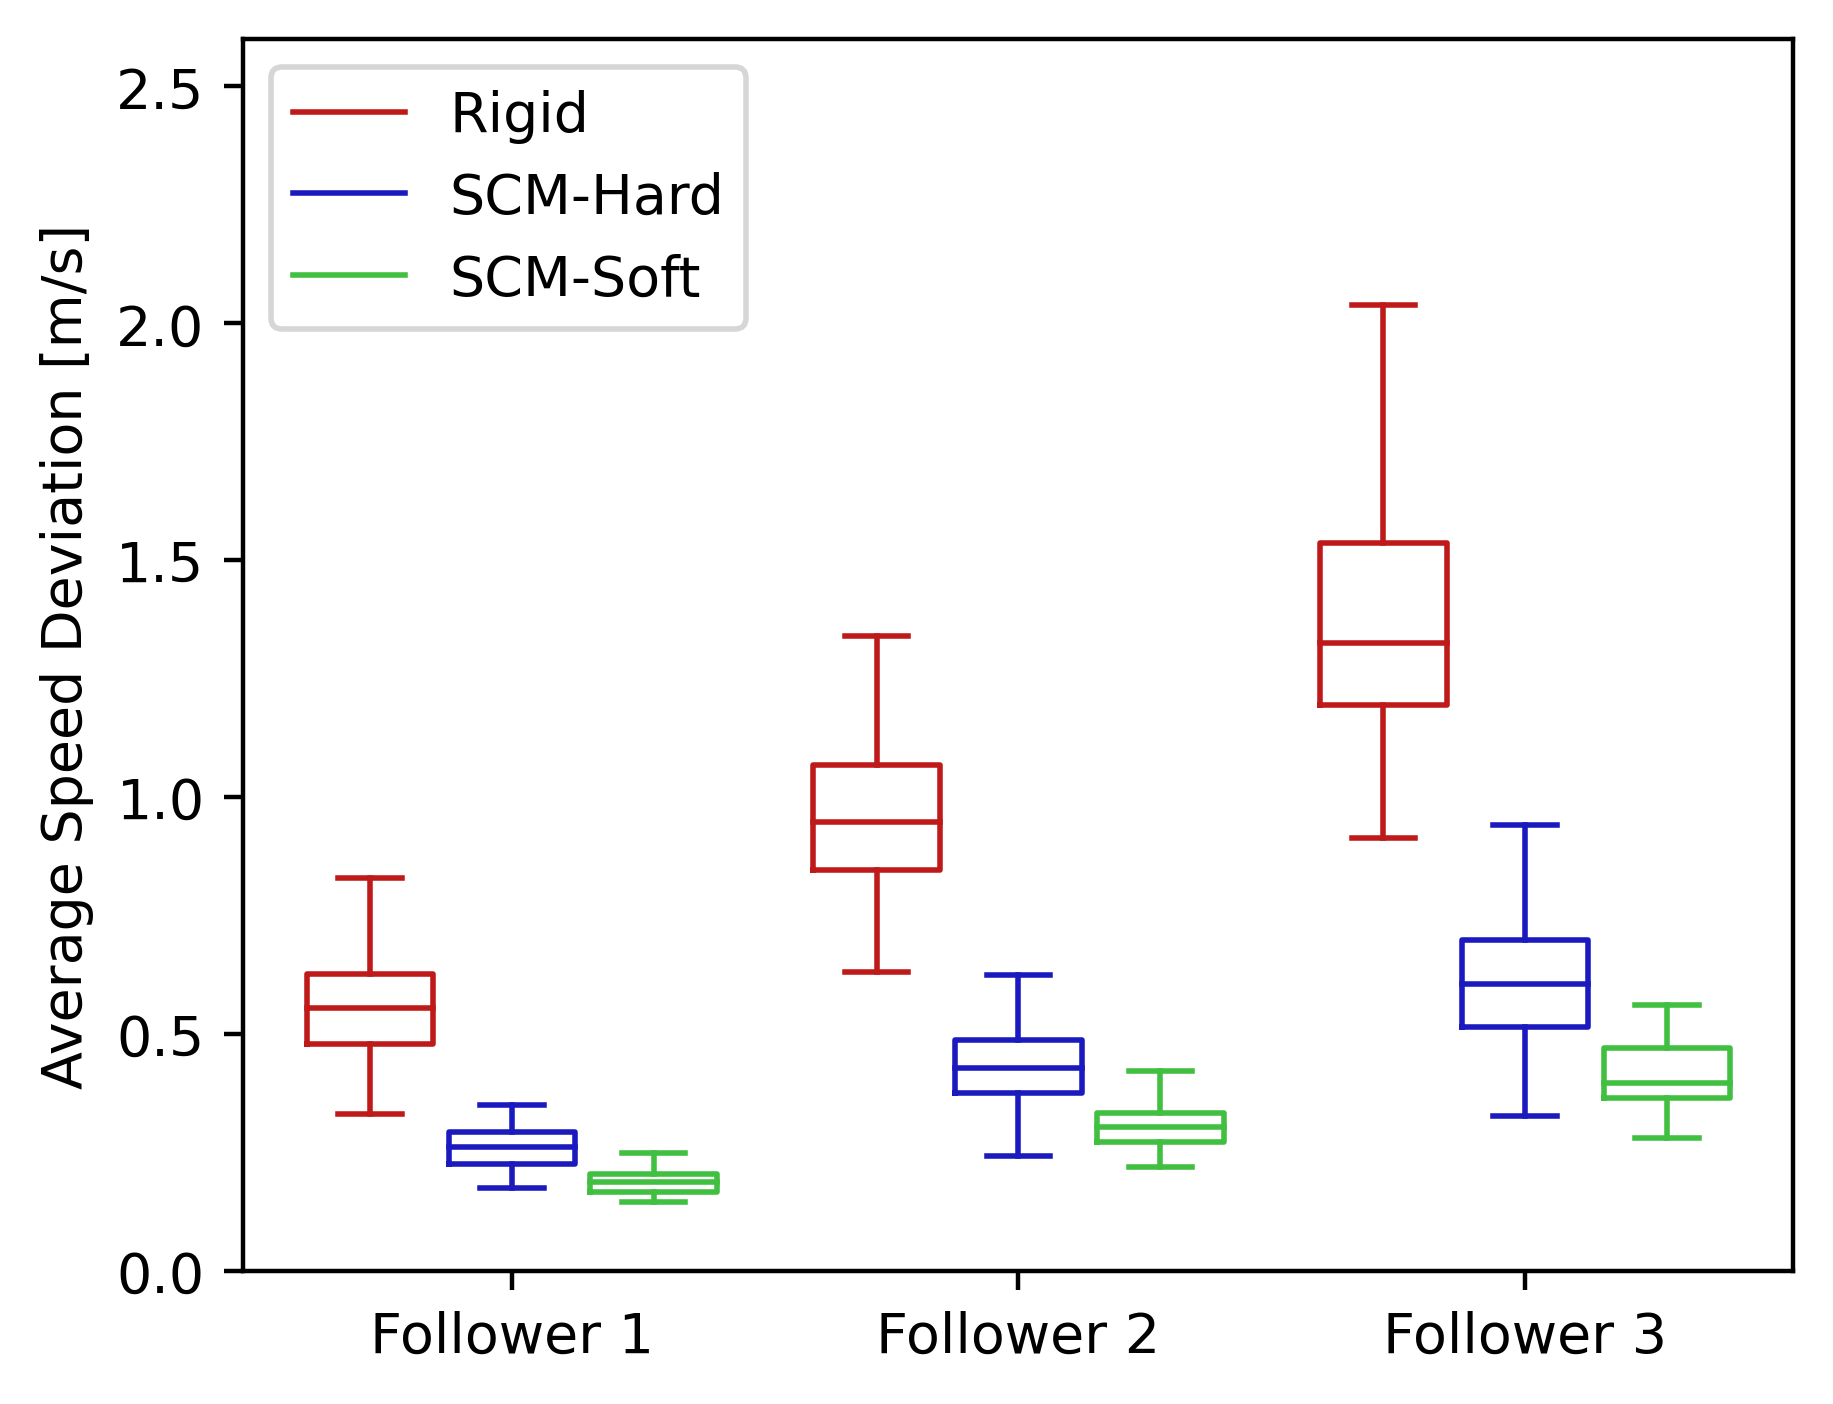
\includegraphics[width=\columnwidth]{Figs/StatisticalAnalysis/metric_speed_avg.png}
        \caption{} \label{fig:metricspeedavg}
    \end{subfigure}
    \begin{subfigure}{0.45\textwidth}
        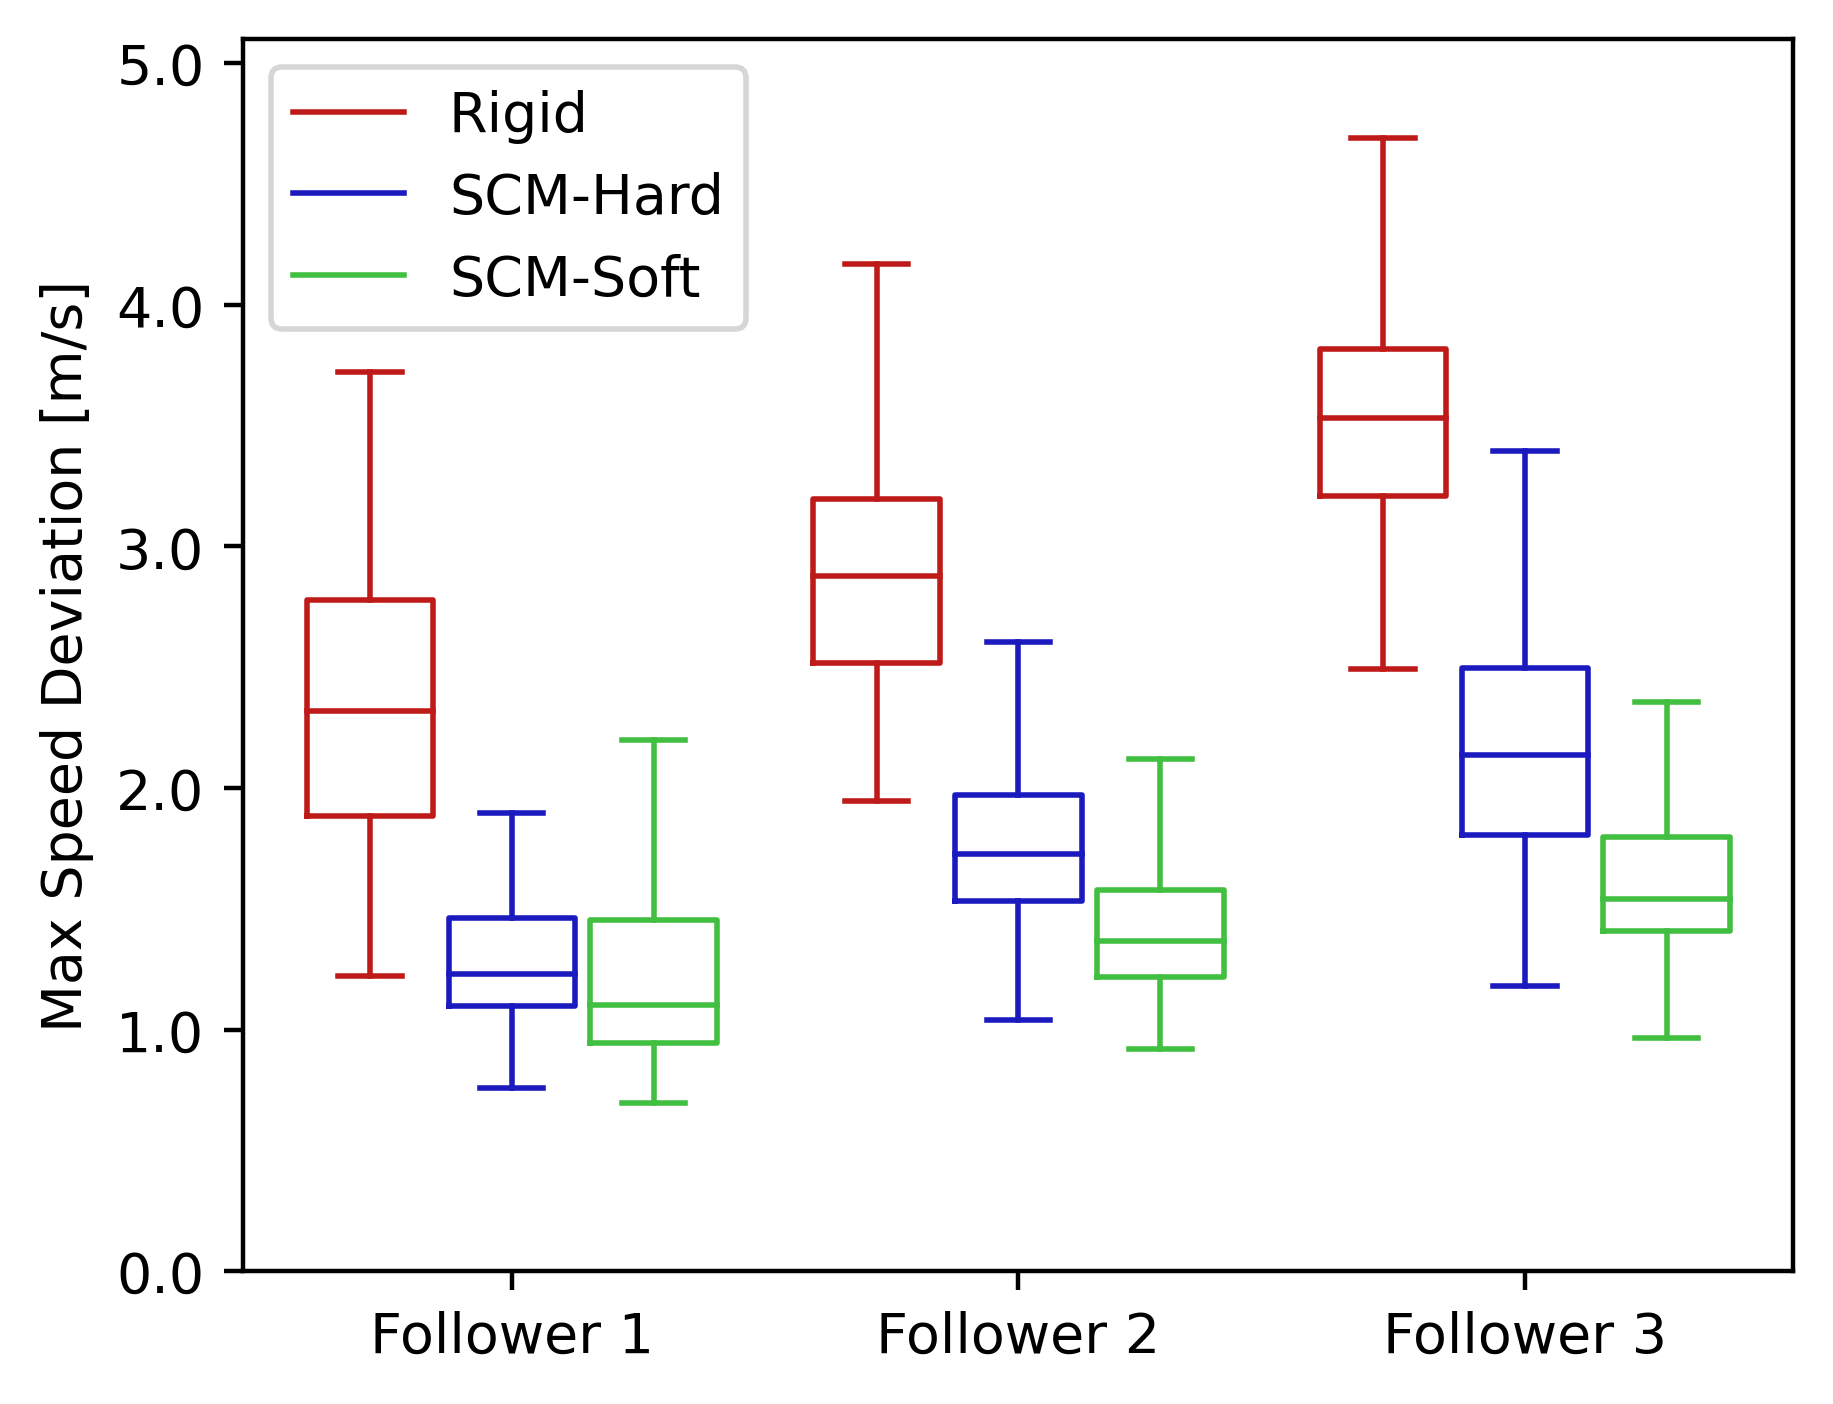
\includegraphics[width=\columnwidth]{Figs/StatisticalAnalysis/metric_speed_max.png}
        \caption{} \label{fig:metricspeedmax}
    \end{subfigure}%
    \caption{Statistics of average and maximum follower absolute speed deviations.}  
    \label{fig:metricspeed}
\end{figure*}

\begin{figure*}
    \centering
    \begin{subfigure}{0.45\textwidth}
        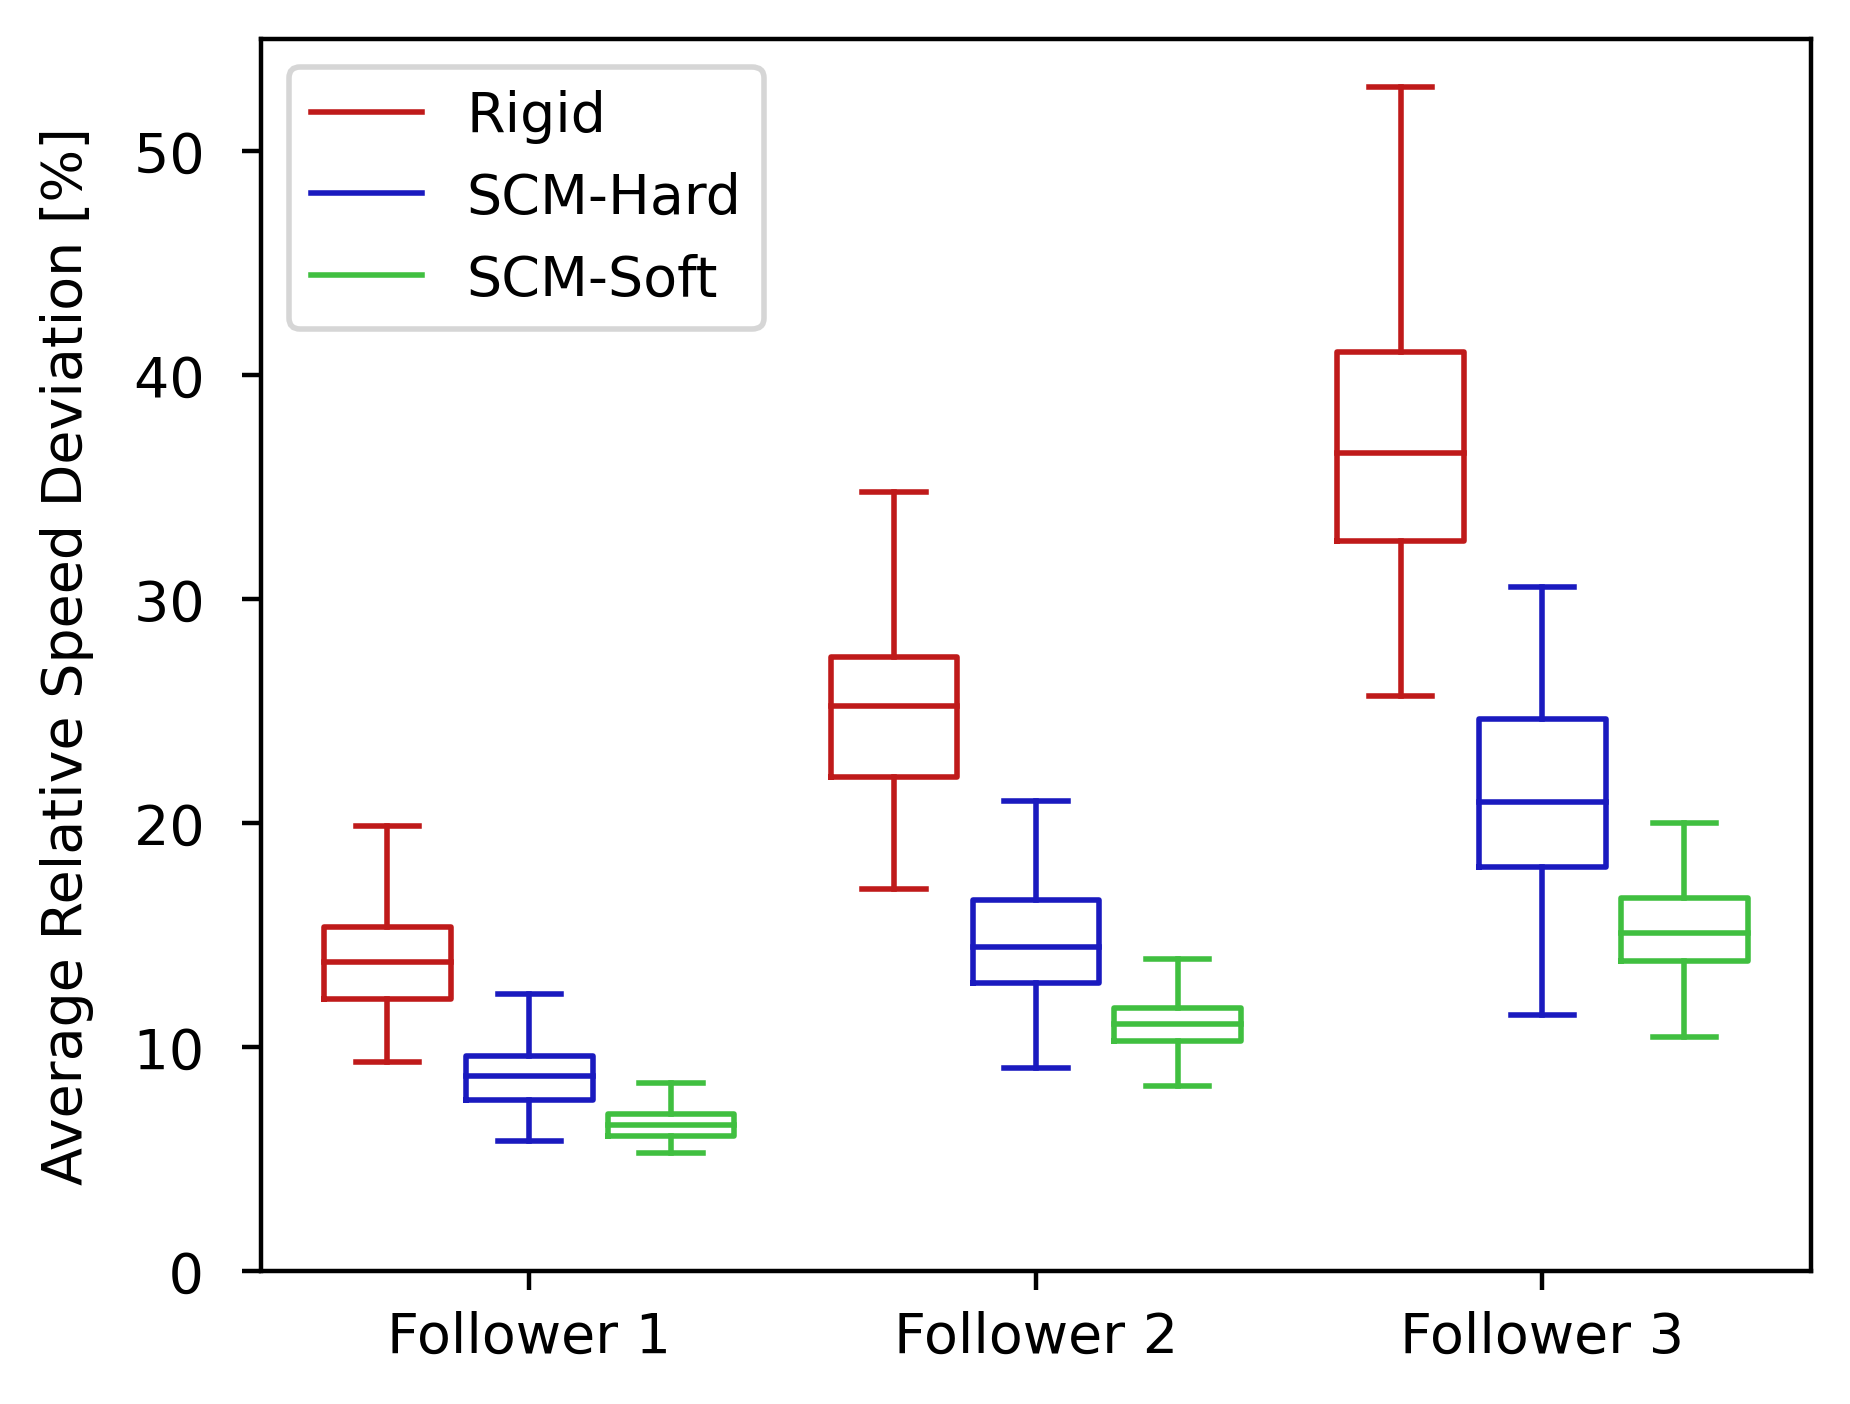
\includegraphics[width=\columnwidth]{Figs/StatisticalAnalysis/metric_rel_speed_avg.png}
        \caption{} \label{fig:metricrelspeedavg}
    \end{subfigure}
    \begin{subfigure}{0.45\textwidth}
        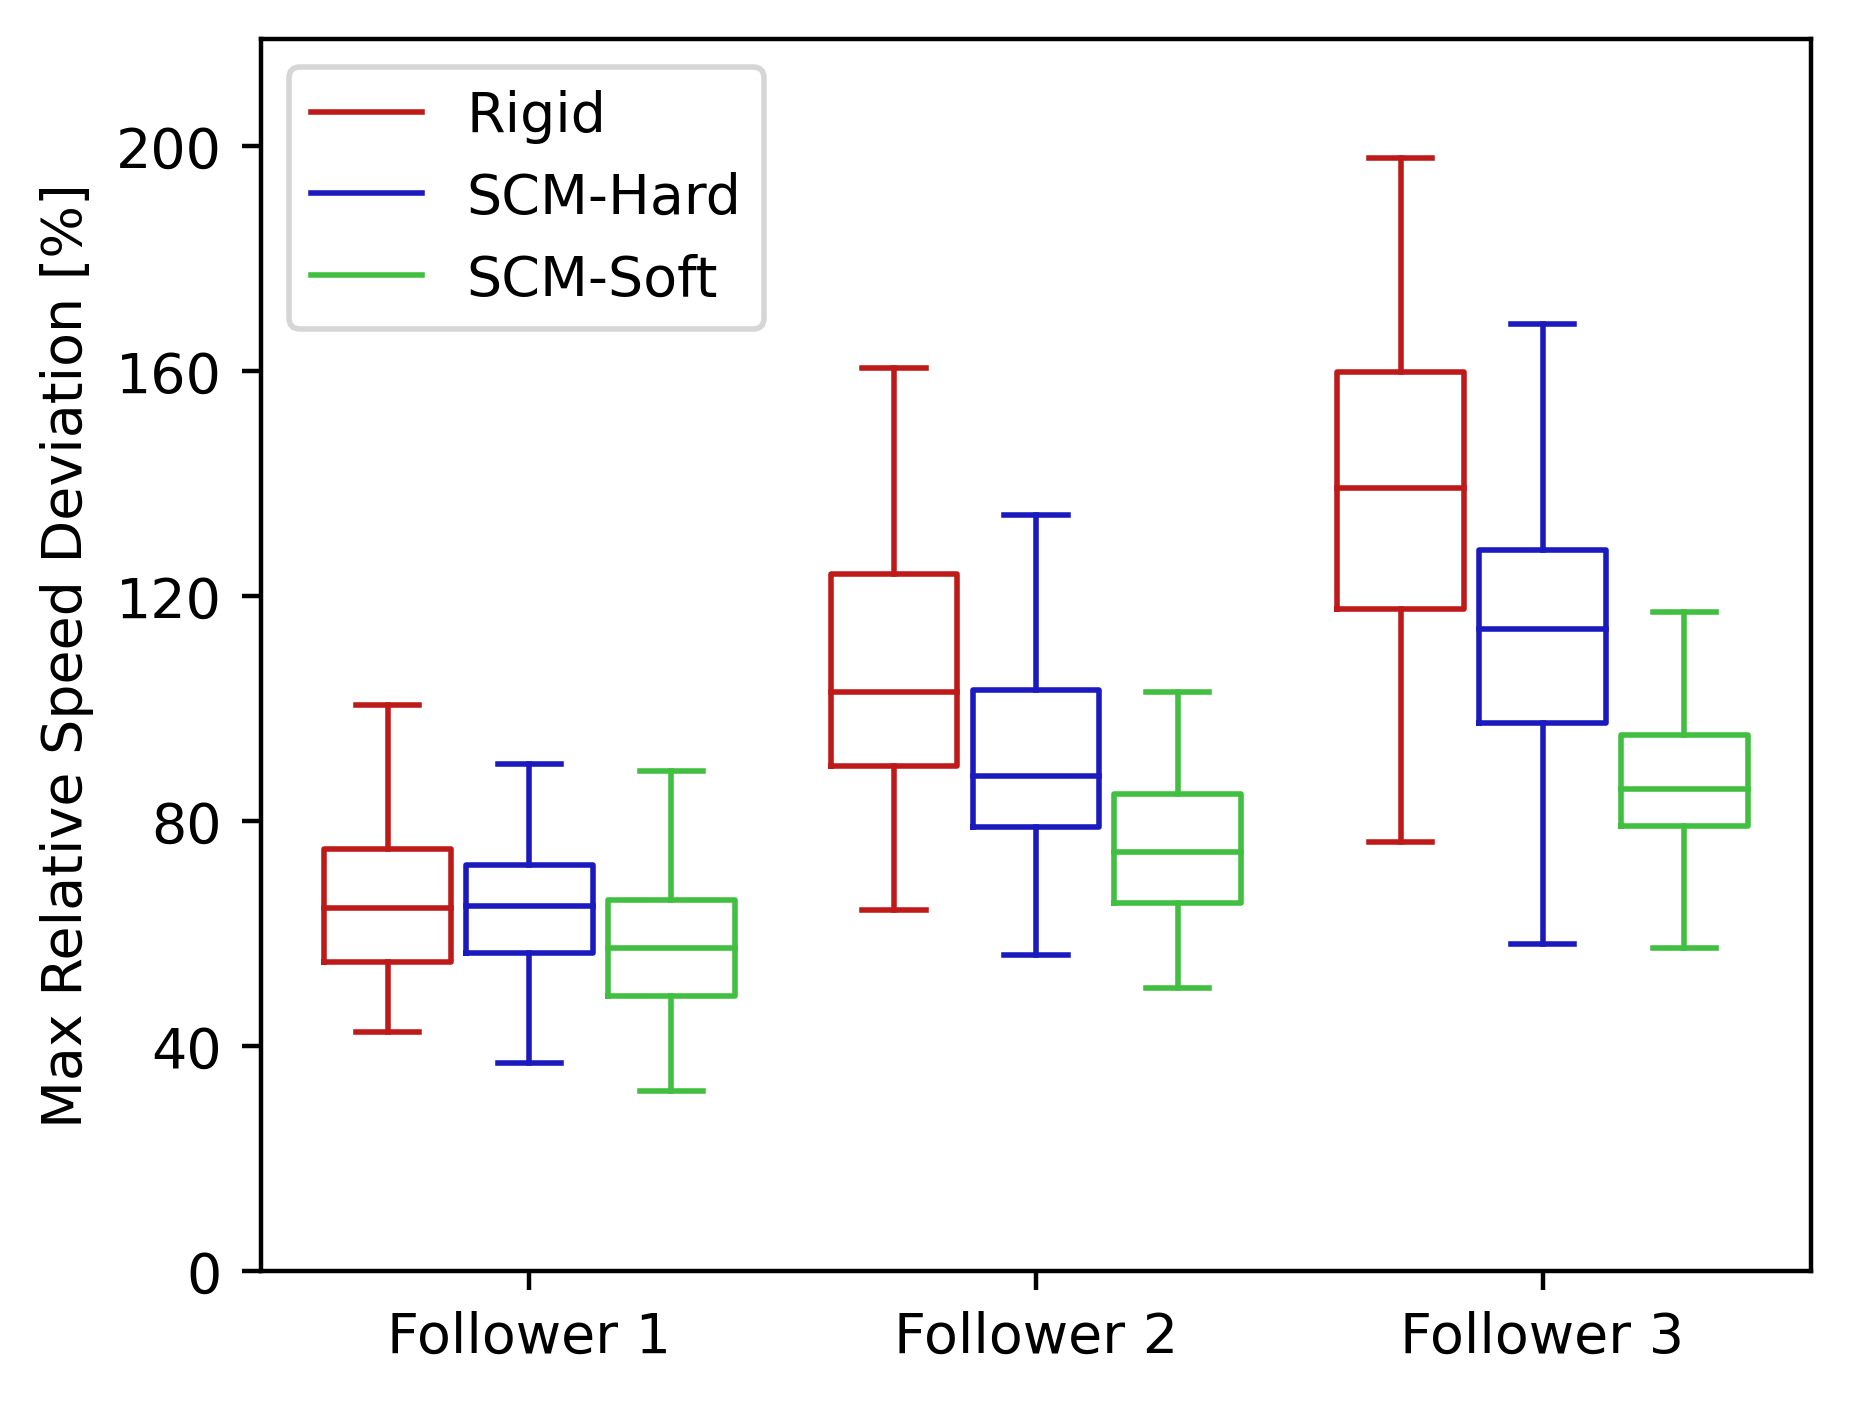
\includegraphics[width=\columnwidth]{Figs/StatisticalAnalysis/metric_rel_speed_max.png}
        \caption{} \label{fig:metricrelspeedmax}
    \end{subfigure}%
    \caption{Statistics of average and maximum follower relative speed deviations.}  
    \label{fig:metricrelspeed}
\end{figure*}

% \begin{figure}
%     \centering
% \end{figure}

% \begin{figure}
%     \centering
%     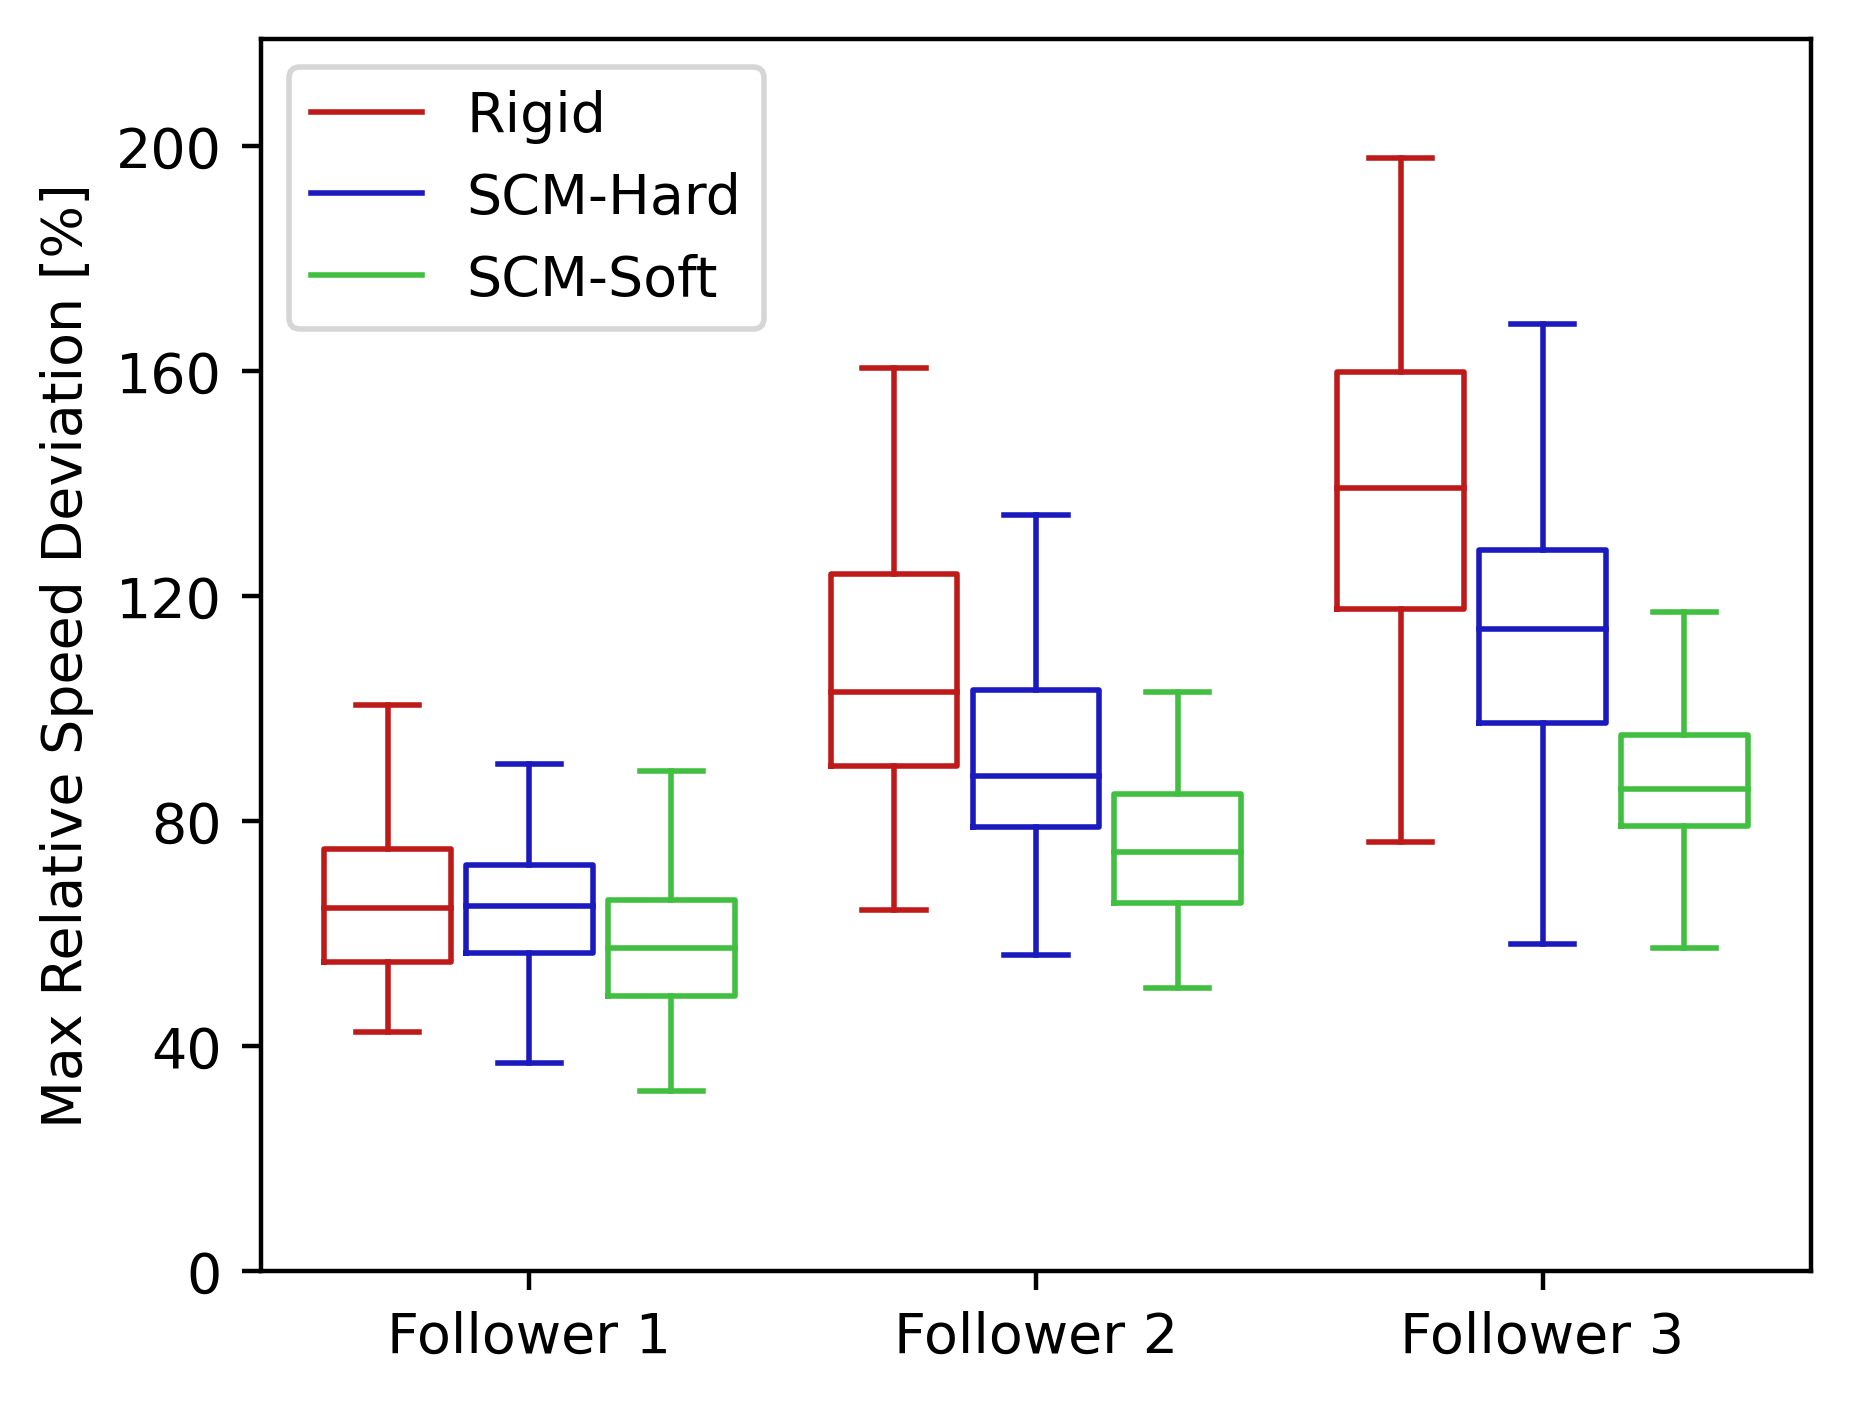
\includegraphics[width=\columnwidth]{Figs/StatisticalAnalysis/metric_rel_speed_max.png}
%     \caption{Maximum error between the followers and leaders velocity profiles, scaled by the speed of the leader at each position along its path.}   
%     \label{fig:metricrelspeedmax}
% \end{figure}

\begin{figure*}
    \centering
    \begin{subfigure}{0.33\textwidth}
        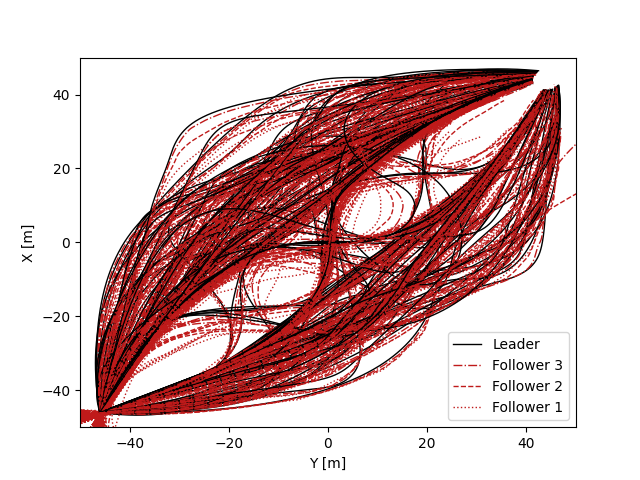
\includegraphics[width=\linewidth]{Figs/StatisticalAnalysis/1L_3F_rigid_128_pos_v5.png}
        \caption{} \label{fig:rigid13pos}
    \end{subfigure}%
    \begin{subfigure}{0.33\textwidth}
        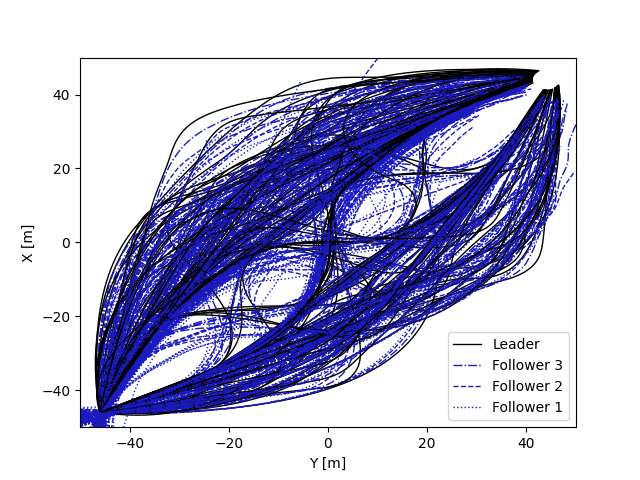
\includegraphics[width=\linewidth]{Figs/StatisticalAnalysis/1L_3F_hard_128_pos_v5.png}
        \caption{} \label{fig:hard13pos}
    \end{subfigure}%
    \begin{subfigure}{0.33\textwidth}
        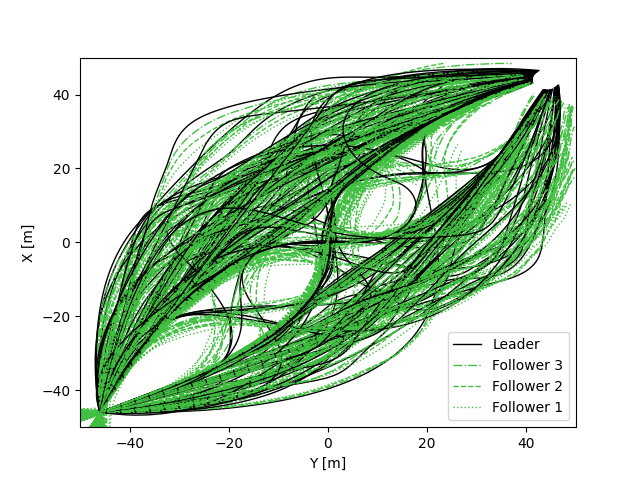
\includegraphics[width=\linewidth]{Figs/StatisticalAnalysis/1L_3F_soft_128_pos_v5.png}
        \caption{} \label{fig:soft13pos}
    \end{subfigure}%
    \caption{Paths of every vehicle on each terrain type: (a) Rigid; (b) SCM-Hard; (c) SCM-Soft.}   
    \label{fig:pathsranksall}
\end{figure*}

\begin{figure*}
    \centering
    \begin{subfigure}{0.33\textwidth}
        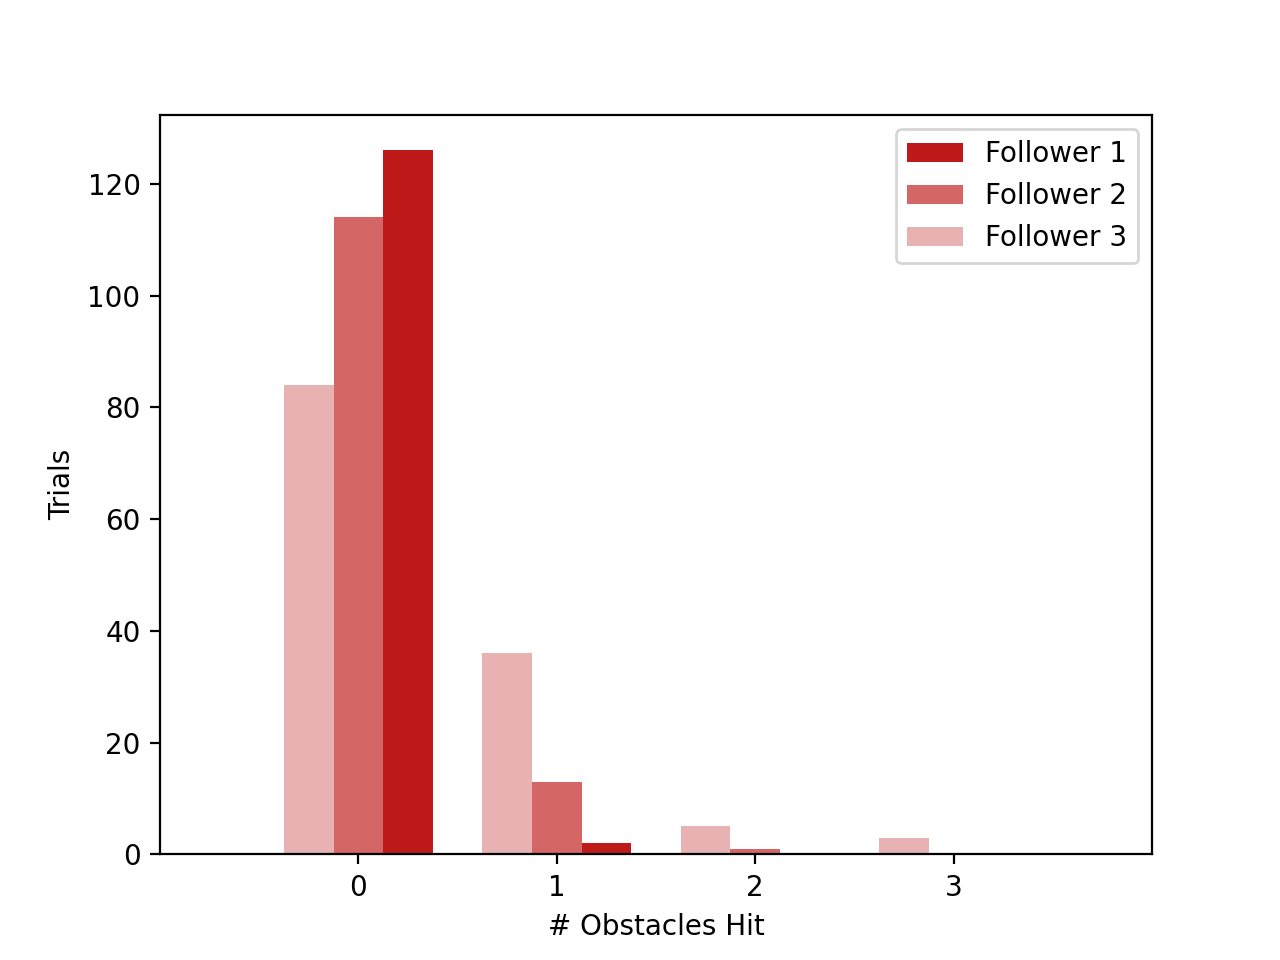
\includegraphics[width=\linewidth]{Figs/StatisticalAnalysis/rigid_histogram.png}
        \caption{} \label{fig:rigidhistogram}
    \end{subfigure}%
    \begin{subfigure}{0.33\textwidth}
        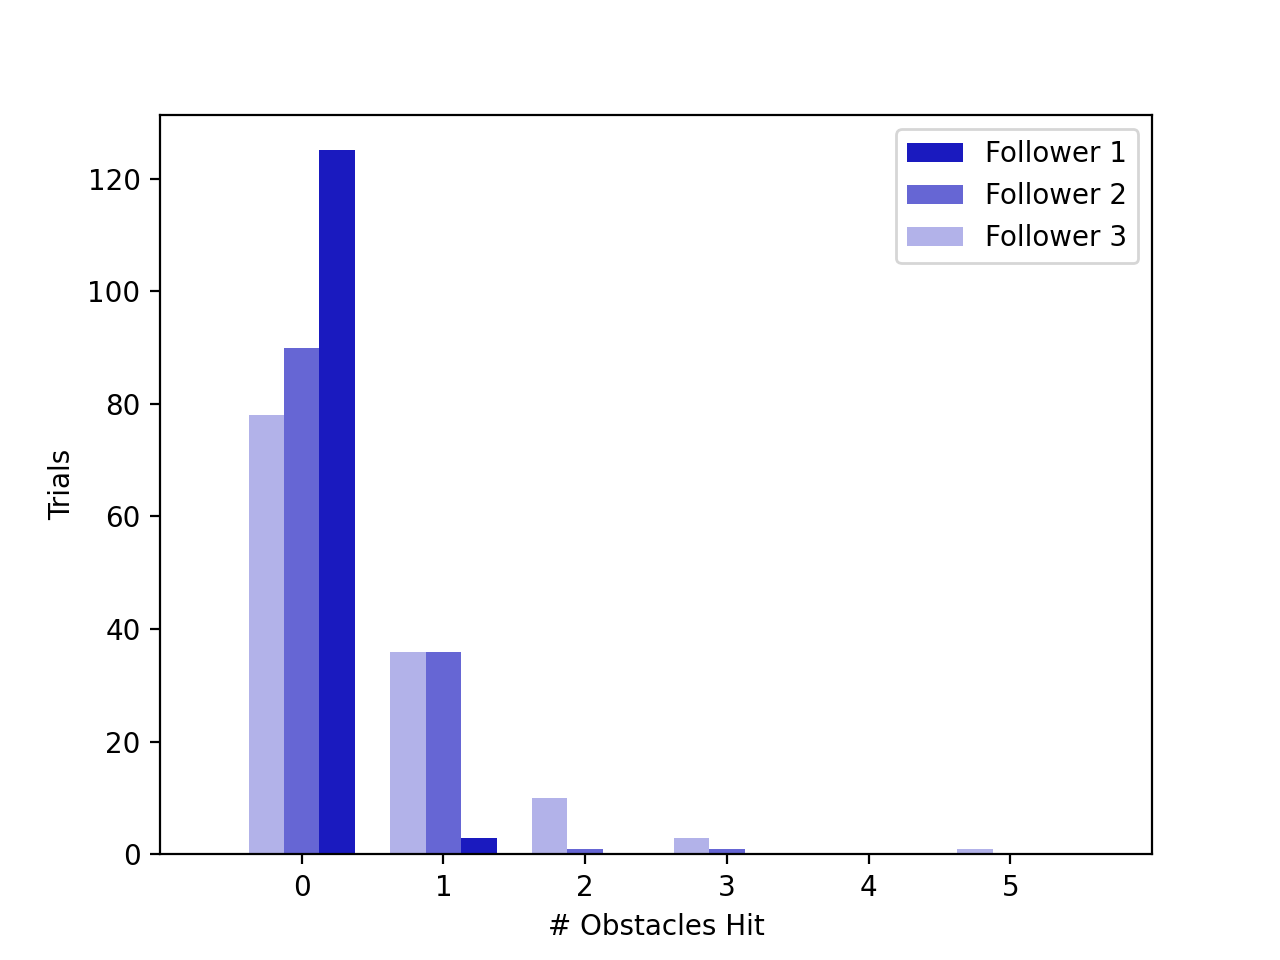
\includegraphics[width=\linewidth]{Figs/StatisticalAnalysis/hard_histogram.png}
        \caption{} \label{fig:hardhistogram}
    \end{subfigure}%
    \begin{subfigure}{0.33\textwidth}
        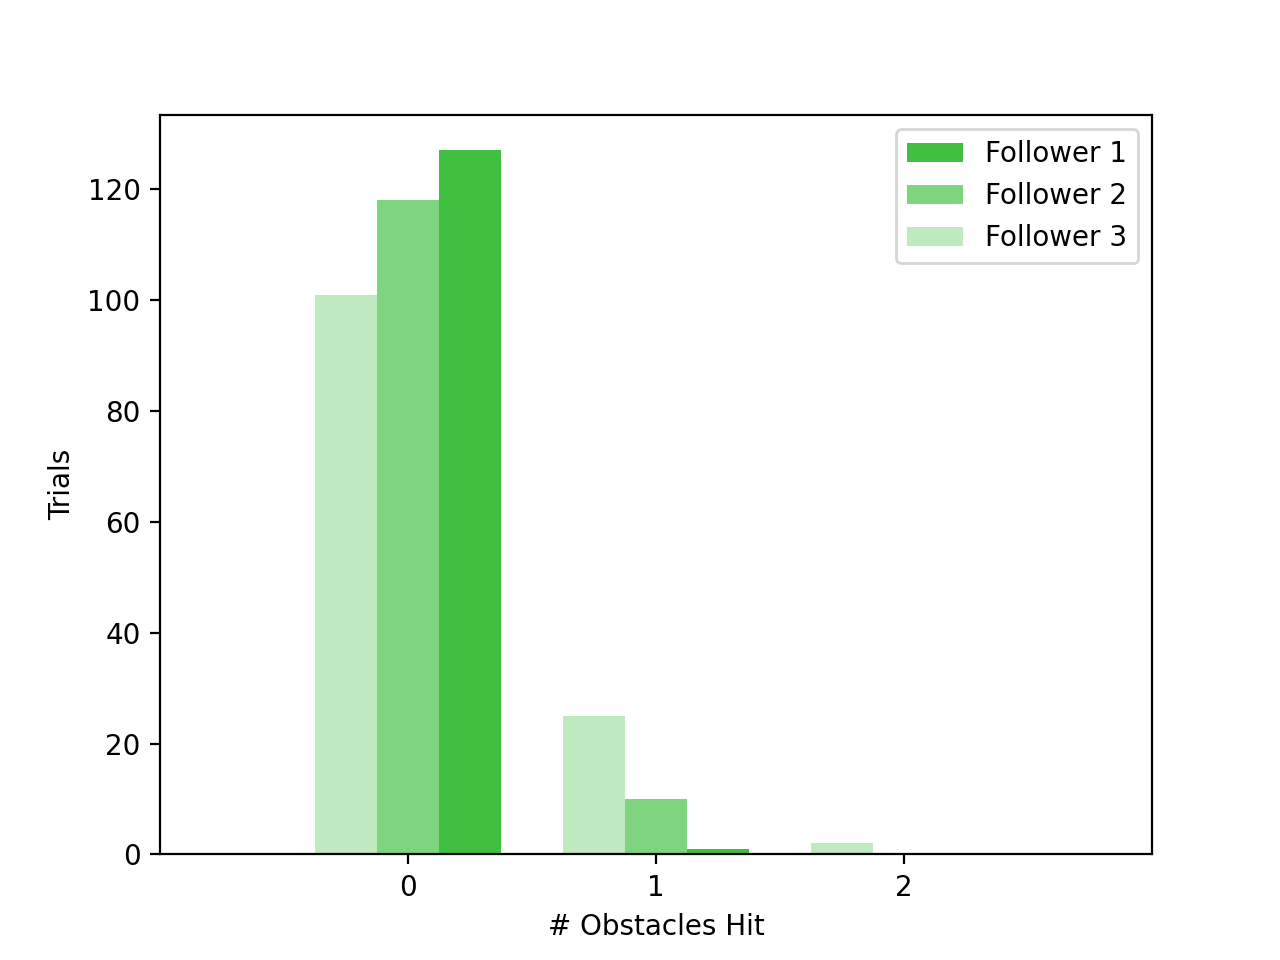
\includegraphics[width=\linewidth]{Figs/StatisticalAnalysis/soft_histogram.png}
        \caption{} \label{fig:softhistogram}
    \end{subfigure}%
    \caption{Number of obstacles hit by each vehicle on the three terrain types: (a) Rigid; (b) SCM-Hard; (c) SCM-Soft.}   
    \label{fig:obstacleshit}
\end{figure*}

%\FloatBarrier

%% ============================================================ 
%% ============================================================ 
\section{CONCLUSIONS. FUTURE WORK}\label{s:conclusion}
This contribution discussed a Chrono-centric simulation platform designed to facilitate the design and testing of control policies for AAs operating in off-road conditions. The platform draws on a physics-based simulation engine; has templates for wheeled and tracked vehicles; enforces space and time coherence; allows for human-in-the-loop scenarios; provides sensor simulation capabilities; has a bridge to ROS; can simulate mobility on fully resolved, continuum, or SCM representations of the terrain; is open source; and is cluster deployable to support multi-AA mobility studies. This software framework is used here to design an RL-based control policy that allows AAs to follow in a convoy formation. The learning took place on rigid terrain but was demonstrated to work when deployed on AAs that operate on deformable SCM soils. The virtual environments used in testing differed in textures and colors from the ones used in the training, thus demonstrating robustness of the inferred policy that relies on inputs from an RGB camera sensor. Unsurprisingly, the fewer AAs in the platoon, the tighter it managed to follow a prescribed path. Looking ahead, we plan to speed up the SCM implementation; augment the sensing simulation support; improve scalability; and use this simulation infrastructure to derive new control policies for off-road AA mobility. 


%% ============================================================

\section*{Acknowledgments}
The Euler supercomputer used in this work contains hardware procured through the Army Research Office DURIP instrumentation grant W911NF1810476. Support for terramechanics research is provided through US Army Research Office project W911NF1910431. Ongoing support for core {\chrono} development is provided by National Science Foundation project CISE1835674. Ongoing support for SynChrono development is provided by National Science Foundation project CPS1739869. Support for the development of \chronomod{Vehicle} was provided by U.S. Army GVSC grant W56HZV-08-C-0236. Support for the development of \chronomod{Sensor} and {\synchrono} has been provided by the SAFER-SIM program, which is funded through a grant from the U.S. Department of Transportation's University Transportation Centers Program (69A3551747131).



%% ============================================================
\bibliographystyle{unsrt}
\bibliography{Bib/refsAutonomousVehicles,Bib/refsMachineLearning,Bib/refsChronoSpecific,Bib/refsCompSci,Bib/refsDEM,Bib/refsFSI,Bib/refsGraphics,Bib/refsMBS,Bib/refsRobotics,Bib/refsSBELspecific,Bib/refsSensors,Bib/refsTerramech,Bib/refsDRL}


%% ============================================================
%%% ============================================================

\clearpage
From this point on is old stuff
\section{FRAMEWORK}\label{s:framework}

%% ============================================================

\subsection{\chronomod{Sensor}}\label{s:ChSensor}

\chrono{} and \synchrono{} and \chronomod{Vehicle} \chronomod{Sensor} is a Project \chrono{} submodule for sensing simulation. Supported sensors include camera, lidar, \gps{}, and \imu{}. Exteroceptive sensing (camera, \lidar{}) leverages headless, off-screen ray-tracing support via \optix{}. \chronomod{Sensor} seeks to generate realistic data that is equivalent to data from its physical counterpart. To this end, \chronomod{Sensor} supports modeling and simulation of the noise and distortion observed on the data streams of physical sensors. Examples of \chronomod{Sensor} used to simulate a scaled autonomous vehicle navigating a closed course are shown below.

\begin{figure}
	\centering
	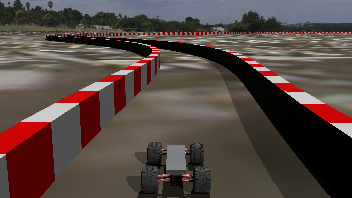
\includegraphics[width=0.8\columnwidth]{Figs/AV-third-person.png}
	\caption{{\small Third person perspective of scaled autonomous vehicle navigating a course using a simulated camera and \lidar{}.}}   
	\label{fig:avthirdperson}
\end{figure}

\begin{figure}
	\centering
	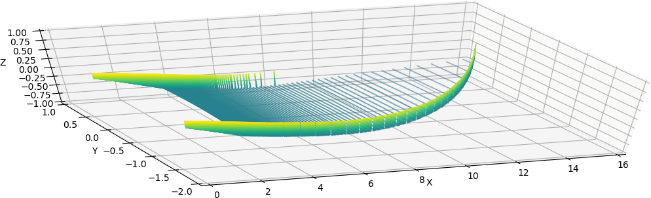
\includegraphics[width=0.8\columnwidth]{Figs/AV-lidar.png}
	\caption{{\small Lidar data showing the course from the perspective of the virtual vehicle. The data is used in the control stack to detect the barriers and determine the desired path.}}   
	\label{fig:avlidar}
\end{figure}

\begin{figure}
	\centering
	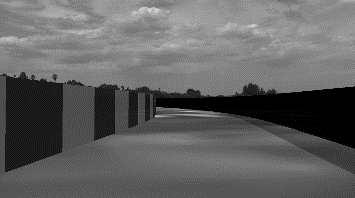
\includegraphics[width=0.8\columnwidth]{Figs/AV-greyscale.png}
	\caption{{\small Image from a simulated grayscale camera mounted to the front of the scaled autonomous vehicle.}}   
	\label{fig:avgreyscale}
\end{figure}

%%============================================================

\subsection{\pychrono{} and \gymchrono{}}\label{s:pyandgym}

\pychrono{} is a package that provides Python bindings for the \chrono{} \api{}. Using an interface compiler (SWIG), the vast majority of the \chrono{} \api{} (multibody dynamics, Vehicle, Sensor, \fea{}, etc.) can be directly accessed from Python. Beyond ease of use, the Python wrapping allows interfacing \chrono{} and ML frameworks for training neural networks. \gymchrono{} provides a set of Robotics and Autonomous Driving environments leveraging \chrono{} for physics simulation and OpenAI gym support for Reinforcement Learning baselines and tools for scalable training.

%%============================================================

\subsection{\synchrono{}}\label{s:synchrono}

\synchrono{} is a software component built on top of \chrono{} that allows for a distributed-memory execution of simulation scenarios that include tens of agents. It builds off the Message Passing Interface (\mpi{}), which allows the toolset to have multiple instances of \chrono{} run simultaneously on a supercomputer/cluster/multi-core setup to allow for the distributed simulation of multiple agents (robots, tracked vehicles, wheeled vehicles, etc.) The paradigm embraced is that of running one \chrono{} agent simulation as one \mpi{} rank, with multiple ranks, say N, communicating through messages to maintain a space and time coherent solution for the N agents participating in the study. This multi-agent form of simulation distribution is possible because of the largely decoupled nature of mobility scenarios. Each agent runs in its own rank and interfaces with its dedicated control stack for software-in-the-loop control. The control stack is fed synthetic data generated by \chronomod{Sensor} and acts upon the environment through \chronomod{Vehicle} control input (throttle, steering, braking, etc.) This “one agent-to-one \chrono{} system” mapping ensures scalability over a monolithic \chrono{} system as shown in the center picture below. The control algorithm or “brain” for each agent is also configurable and can vary from complex algorithms that collect a variety of sensor data, to controls based on empirical models, to human-driven control in scenarios that are simple enough to allow real-time simulation.

\begin{figure}
	\centering
	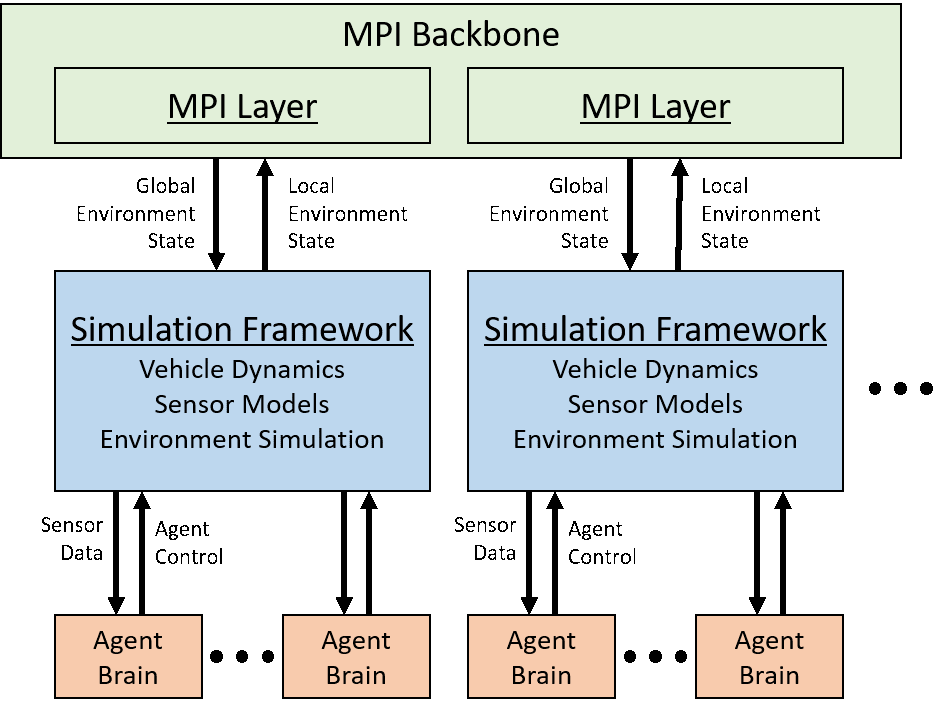
\includegraphics[width=0.8\columnwidth]{Figs/MPI-schematic.png}
	\caption{{\small Schematic of the \synchrono{} framework. Decisions are passed to the \chrono{} system for dynamics simulation and the outcome of the dynamics simulation is synchronized between ranks using \mpi{}.}}   
	\label{fig:mpischematicold}
\end{figure}

\begin{figure}
	\centering
	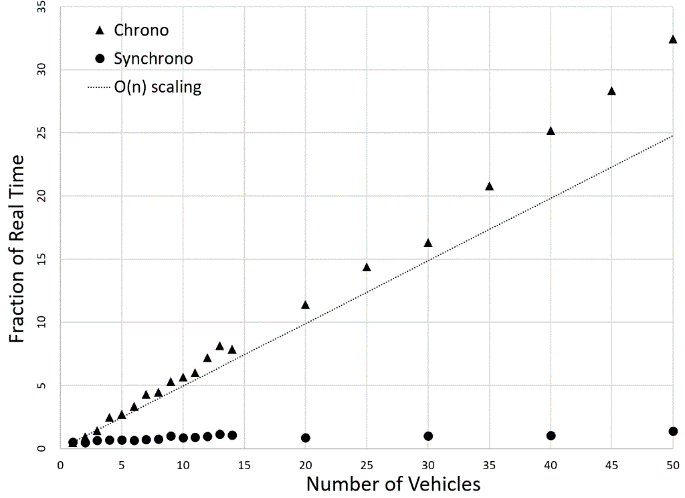
\includegraphics[width=0.8\columnwidth]{Figs/Syn-Chrono-Scaling.png}
	\caption{{\small Scaling comparison between \chrono{} and \synchrono{}. By running each simulation in parallel \synchrono{} handles scenarios with large numbers of vehicles much faster and closer to real-time than \chrono{}.}}   
	\label{fig:synchronoscalingold}
\end{figure}

\begin{figure}
	\centering
	\includegraphics[width=0.8\columnwidth]{Figs/Syn-Platoon.png}
	\caption{{\small Image of a collection of agents in a shared, coherent virtual world.}}   
	\label{fig:synplatoonold}
\end{figure}

\subsection{ROS \chrono{} Control Interface}\label{s:roscontrolinterface}

To allow for the seamless testing of control algorithms that are intended to be easily transferred to real vehicles or robots, the toolset provides a \ros{} control interface that is exposed in \synchrono{}. Using \tcp{}, messages from \synchrono{} (i.e. sensor data packets), are sent into a \ros{} node on the same system running the vehicle control stack. This node also listens to the \ros{} control messages that are produced and sends them back to \synchrono{} for input to the \chrono{} agents. With this \ros{} interface, the tested control stack is independent of the \synchrono{} platform (i.e. can be run on a different operating system or architecture) and can be tested with inputs replicating those from reality, such as sensor and/or V2X communication data.

\clearpage

%% ============================================================
\section{Demonstration}\label{s:demonstration}
\todo[inline]{Asher's details on the proposed demonstration: the goal of the demonstration is to show a multi-agent simulation of vehicles driven with policies learned using RL in PyChrono. To accomplish this we will train a single agent to participate in a follow-the-leader convoy through a narrow path. It will be trained on rigid terrain until an optimal policy is found. We can then refine the policy on SCM terrain. The trained policy will be deployed for all vehicles in SynChrono. We can remove the need for sensing the SCM terrain if we using a simulated vehicle-to-vehicle message from the lead vehicle. I think it would be more interesting to include a camera as input and remove the need to know the position of the lead vehicle. Final decision on that TBD. The study will then be on how that policy is deployed in SynChrono and how it responds to perturbations in the form of ruts in the soil.}

\todo[inline]{DN - Training for convoy vehicle: sensor (GPS+Camera) fusion + rigid terrain + ghost vehicle(s). Training for lead vehicle: path (perhaps way points) + sensor fusion + obstacles}

\todo[inline]{DN: SynChrono scaling analysis on SCM with 1, 2, 4, 8, etc. vehicles; half going NS, half EW. SCM deformable terrain; deformable terrain shown in simulation and also picked up by sensor.}

%% ============================================================

\begin{figure}
    \centering
    \includegraphics[width=0.8\columnwidth]{Figs/M113Fording.png}
    \caption{{\small M113 fording maneuver demonstrating \chrono{} and \chronomod{Vehicle} capabilities.}}   
    \label{fig:m113fording}
\end{figure}

\begin{figure}
    \centering
    \includegraphics[width=0.8\columnwidth]{Figs/HMMWV-Granular.png}
    \caption{{\small HMMWV with flexible tires navigating granular terrain demonstrating vehicle dynamics, flexible body dynamics, and parallel computing support in \chrono{}.}}   
    \label{fig:hmmwvgranular}
\end{figure}

\begin{figure}
    \centering
    \includegraphics[width=0.8\columnwidth]{Figs/GymChrono-Pilars.png}
    \caption{{\small \gymchrono{}-enabled learning with simulated sensor data provided by \chronomod{Sensor} gradually allows the vehicle to understand how to avoid random obstacles placed in its path}}   
    \label{fig:gymchronopillars}
\end{figure}


This contribution outlines the current state of a BSD3 open-source simulation toolset whose goal is to assist practitioners in endowing autonomous agents with artificial intelligence; i.e., producing control strategies that enable heterogeneous teams of robots and wheeled/tracked vehicles to operate in off-road conditions in a coordinated fashion towards accomplishing a shared task. The toolset draws on: \chrono{} , which provides multi-physics support for agent modeling; \chronomod{Sensor}, which produces synthetic data for simulating sensing; \pychrono{} and \gymchrono{}, which provide support for machine learning; \synchrono{}, a software component for software/hardware/human in the loop studies that include multiple agents; and the \ros{}-\chrono{} Control Interface, which allows the toolset to converse with the software libraries/utilities provided by \ros{} . The reinforcement learning (RL) support provided through \gymchrono{} is demonstrated in conjunction with an RL experiment in which a HMMWV-type vehicle learns how to avoid road obstacles while moving in a convoy.


\section*{Acknowledgments}
This work was supported by a U.S. Army TARDEC project. \chrono{} development was supported in part by U.S. Army TARDEC Rapid Innovation Fund grant No. W911NF-13-R-0011, Topic No. 6a, ``Maneuverability Prediction''. 







%% *******************************************************************
%% Examples for including single- and double-column figures and tables
%% *******************************************************************

%\begin{figure}
%	\centering
%	\includegraphics[width=0.8\columnwidth]{Figs/hmmwv_1.png}
%	\caption{{\small A figure spanning a single column. The caption should wrap nicely here.}}   
%	\label{fig:one}
%\end{figure}

%\begin{figure*}
%	\centering
%	\includegraphics[width=0.75\textwidth]{Figs/hmmwv_1.png}
%	\caption{{\small A figure spanning the entire paper width}}    
%	\label{fig:two}
%\end{figure*}

% \begin{table}
% \begin{center}
% 	\begin{tabular}{||c |c | c||} 
% 		\hline
% 		Test  & Terrain  & Controller Vehicle \\
% 		Number &  Type & Model\\ [0.5ex] 	
% 		\hline\hline
% 		1 & Rigid & 2-DOF \\ 
% 		\hline
% 		2 & Rigid & 14-DOF \\
% 		\hline
% 		3 & Granular & 2-DOF \\
% 		\hline
% 		4 & Granular & 14-DOF \\
% 		\hline
% 	\end{tabular}
% \end{center}
% \caption{A table spanning a single column. The caption should wrap nicely here.}
% \label{t:one}
% \end{table}

% \begin{table*}
% 		\centering
% \begin{tabular}{ ||p{6cm}|p{1.8cm}|p{1.8cm}|p{1.8cm}|p{1.8cm}||  }
% 		\hline
% 		Test Number & 1 & 2 & 3 & 4\\
% 		\hline
% 		Controller Model & 2-DOF & 14-DOF & 2-DOF & 14-DOF\\
% 		\hline
% 		Terrain & Rigid & Rigid & Granular & Granular\\
% 		\hline
% 		Time to Target (s)  & 26.67 & 26.15 & 28.32 & 28.03\\ 
% 		\hline
% 		Minimum Obstacle Distance (m) & 0.897 & 5.462 & 3.491 & 4.721\\
% 		\hline
% 		Controller Effort & 0.0340 & 0.0340 & 0.0340 & 0.0306\\
% 		\hline
% 		Max. Lateral Acceleration (m/s$^{2}$)& 2.78 & 1.57 & 2.47 & 2.33 \\
% 		\hline
% 		Avg. Lateral Acceleration (m/s$^{2}$) &0.54 & 0.51 & 0.55 & 0.46\\
% 		\hline
% \end{tabular}
% \caption{A table spanning both columns.}
% \label{t:two}
% \end{table*}

%% ============================================================


\end{document}

